\documentclass[a4paper,11pt]{article}
\usepackage[table]{xcolor}




\usepackage[T1]{fontenc}
\usepackage[normalem]{ulem}
\usepackage{mathtools}
\usepackage{blkarray,bigstrut} 
\usepackage{graphicx,wrapfig,lipsum}
\usepackage{tcolorbox}
\usepackage{enumitem}
\usepackage{array}
\usepackage{algorithm}
\usepackage{algorithmic}
\usepackage{mathpartir}
\usepackage{multirow}
\usepackage{hyperref}
\usepackage{amssymb}
\usepackage{subcaption}
\usepackage{stmaryrd}
\usepackage{color} 


\usepackage{tikz}
\usetikzlibrary{snakes}
\usetikzlibrary{svg.path} 
\usetikzlibrary{calc} 
\usetikzlibrary{shapes}
\usetikzlibrary{shapes.geometric}
\usetikzlibrary{arrows.meta}
\usetikzlibrary{arrows}
\usetikzlibrary{decorations.text,decorations.markings}
% % % % 

%%%%%%%%%%Packages for adaoption%%%

% \usepackage{amsthm} 

%Packages

\input{ldefs}
\newcommand{\highlight}[1]{\textcolor[rgb]{.0,0.0,1.0}{ #1}}

\usetikzlibrary{shapes,arrows}
\newcommand{\THESYSTEM}{\textsf{PsRB}}

% Define block styles
\tikzstyle{decision} = [diamond, draw, fill=blue!20, 
    text width=4.5em, text badly centered, node distance=3cm, inner sep=0pt]
\tikzstyle{block} = [rectangle, draw, fill=blue!20, 
    text width=5em, text centered, rounded corners, minimum height=4em]
\tikzstyle{line} = [draw, -latex']
\tikzstyle{cloud} = [draw, ellipse,fill=red!20, node distance=3cm,
    minimum height=2em]

\begin{document}
\title{Path Sensitive Reachability Bound}

\author{}

\date{}

\maketitle
%
\tableofcontents

% \input{example_cousot}
% \clearpage
% %
\section{{While Language}}
\label{sec:language}
\subsection{Labeled Language}
\[
\begin{array}{llll}
\mbox{Arithmetic Operators} 
& \oplus_a & ::= & + ~|~ - ~|~ \times 
%
~|~ \div ~|~ \emax ~|~ \emin
\\  
\mbox{Arithmetic Expression} 
& \aexpr & ::= & 
n ~|~ {x} ~|~ \aexpr \oplus_a \aexpr  
 ~|~ \elog \aexpr  ~|~ \esign \aexpr
\\
\mbox{Boolean Expression} & \bexpr & ::= & 
%
\etrue ~|~ \efalse  ~|~ \neg \bexpr
 ~|~ \bexpr \land \bexpr
%
~|~ \bexpr \lor \bexpr
~|~ \aexpr \leq \aexpr 
~|~ \aexpr < \aexpr 
~|~ \aexpr = \aexpr 
\\
\mbox{Expression} & \expr & ::= & v ~|~ \aexpr ~|~ \bexpr ~|~ [\expr, \dots, \expr]
\\  
%
\mbox{Value} 
& v & ::= & { n \in \mathbb{N}^{\infty} ~|~ \etrue ~|~ \efalse ~|~ [] ~|~ [v, \dots, v]} \\
%
% \\%
\mbox{Label} 
& l & \in & (\mathbb{N} \cup \{\lin, \lex\}) 
\\ 
%
\mbox{Labeled Command} 
& {c} & ::= &  
\clabel{\assign{x}{\expr}}^l 
~|~  \clabel{\eskip}^l
~|~ \ewhile \clabel{\bexpr}^{l} \edo ({c})
~|~ \eif(\clabel{\bexpr}^{l} , {c}, {c}) 
~|~ {c};{c}  
\\ 
\mbox{Event} 
& \event & ::= & 
({x}, l, v) ~ \mbox{Assignment Event} 
% \\
% &&& 
~|~(\bexpr, l, v) ~ \mbox{Testing Event}
\\
\mbox{Trace} & \trace
& ::= & [] ~|~ \trace :: \event
\\
\end{array}
\]
We denote by $\infty$ a value s.t. $n < \infty $ for all $n \in \mathbb{N}$.
We use following notations to represent the sets of corresponding terms:
\[
\begin{array}{lll}
\vardom & : & \mbox{Set of Variables}  
\\ 
%
\booldom & : & \mbox{Set of Boolean Expressions}  
\\ 
%
\cdom & : & \mbox{Set of Commands} 
\\ 
%
\eventset  & : & \mbox{Set of Events}  
\\
%
\eventset^{\asn}  & : & \mbox{Set of Assignment Events}  
\\
%
\eventset^{\test}  & : & \mbox{Set of Testing Events}  
\\
%
\ldom  & : & \mbox{Set of Labels}  
\\
%
\highlight{\ftdom} & : & \mbox{\highlight{Set of All Finite Execution Traces}}
\\
\highlight{\inftdom} & : & \mbox{\highlight{Set of Infinite  Execution Traces}}
\\
\highlight{\tdom} & : & \mbox{\highlight{Set of All Finite Or Infinite  Execution Traces}}
\\ 
%
\inpvar(c) & : & \mbox{Set of Program $c$'s Input Variables}  
\\
%
\ftdom_0(c) & : & \mbox{Set of Program $c$'s Initial Traces.}
\\ & & \mbox{Each initial trace $\trace_0 \in \ftdom_0(c)$ is finite and every input variable of the program $c$ has an initial value in $\trace_0$.}
\end{array}
\]
%
\subsection{{Trace-based Operational Semantics}}
\label{sec:operational_semantics}
\paragraph{Event}
An event is a triple.
Its first element is the variable name $x$,
or a boolean expression (from the guard of if or while command), 
following by 
 the label, $l$ associated to this command and the value assigned to the variable.

 We have two kinds of events: \emph{assignment events} and \emph{testing events},
 and we use $\eventset^{\asn}$ and $\eventset^{\test}$ to denote the set of all assignment events and testing events, respectively.

 An \emph{assignment event} tracks the execution of an assignment and consists of the assigned variable, the label of the command that generates it, the value assigned to the variable.

 A \emph{testing event} tracks the execution of if and while commands, specifically the evaluation of the boolean expression $b$ in the guard of a $\eif(\clabel{b}^l, c_1, c_2)$ command or $\ewhile \clabel{b}^l \edo c$.
 It consists of the boolean expression $b$ in the guard of the command, the label of the guard, the result of evaluating the guard.
%
\[
\begin{array}{llll}
  \mbox{Event} 
  & \event & ::= & 
  ({x}, l, v) ~ \mbox{Assignment Event} 
  ~|~(\bexpr, l, v) ~ \mbox{Testing Event}
\end{array}
\]
Event projection operators $\pi_i$ projects the $i^{th}$ element from an event: 
% \\
$\pi_i : 
\eventset \to \vardom \cup \booldom \cup \ldom $

\paragraph{Trace.}
%
A trace $\trace \in \tdom $ is a list of events, 
collecting the events generated along the program execution. 
\[
\begin{array}{llll}
\mbox{Trace} & \trace
& ::= & [] ~|~ \trace :: \event
\end{array}
\]
A trace can be regarded as the program history, 
which records all the evaluations for assignment commands and guards in $\eif$ and $\ewhile$ command.
\\
\highlight{If a program doesn't terminate when executing under some initial trace, it produces an infinite trace $\trace \in \tdom^{\infty}$.
$\tdom^{\infty}$ is the set of all finite or infinite traces.}
\\
$\tracecat: \mathcal{T} \to \mathcal{T} \to \mathcal{T}$ is the trace concatenation operator, which combines two traces,
and $\vcounter : \mathcal{T} \to \mathbb{N} \to \mathbb{N}$ is the counting operator, 
which counts the occurrence of a labeled variable in the trace. When the input trace is infinite, it returns $\infty$.
$\event \in \trace $ or $\event \notin \trace $ denotes that $\event$ belongs to $trace$ or not.
All the definition details are in the appendix.
%
The counter operator is abused when the input is a sequence of labels $L = (l_1, \cdots, l_n)$ by counting the occurrence
of this sequence in trace. Specifically,
$\vcounter(\trace :: (\_, l_1, \_) :: \cdots :: (\_, l_n, \_), L ) \triangleq \vcounter(\trace, L) + 1$
and $\vcounter(\trace :: (\_, l, \_), L ) 
\triangleq \vcounter(\trace, L) ~ l \neq l_n$, etc.
The operator $\tlabel : \tdom \to \mathcal{P}{(\ldom)}$ gives the set of labels in every event belonging to a trace.
$\tlabel{(\trace  :: (\_, l, \_)])} \triangleq \{l\} \cup \tlabel{(\trace )}$ and $\tlabel({[ ]}) \triangleq \{\}$.
%
\paragraph{Environment.} $\env : {\ftdom}  \to \vardom \to(\mathbb{N} \cup \{\bot\})$
\[
\begin{array}{llll}
\env(\trace  \traceadd (x, l, v)) x \triangleq v
&
\env(\trace \traceadd (y, l, v)) x \triangleq \env(\trace) x, y \neq x
&
\env(\trace \traceadd (b, l, v)) x \triangleq \env(\trace) x
&
\env({[]} ) x \triangleq \bot
\end{array}
\]
%
\begin{lem}[Initial Traces]
  \label{lem:initial_trace}
  \[
    \forall c \in \cdom, \trace \in \ftdom \st \trace \in \ftdom_0(c) \iff 
    \forall x \in \inpvar(c) \st \env(\trace_0) x \neq \bot
    \]
\end{lem}
%
\paragraph{Configuration.}
%
\paragraph{Expression Semantics}
The evaluation notation for arithmetic expression is $\econfig{} : \mathcal{A} \to \tdom \to \mathcal{V}$.
The $\econfig{\aexpr}(\trace)$ evaluates an arithmetic expression $\aexpr$ under trace $\trace$ following the arithmetic expression evaluation rules in Figure~\ref{fig:aexpr-eval}.
\begin{figure}
\begin{mathpar}
  \boxed{ \econfig{} \, : \, \mbox{Arithmetic Expression $\to$ Trace $\to$ Arithmetic Value}}
  \\
  \inferrule{ 
    \empty
  }{
   \econfig{n} (\trace)
   = n
  }
  \and
  \inferrule{ 
    \env(\trace) x = v
  }{
   \econfig{x} 
   = v
  }
  \and
  \inferrule{ 
    \econfig{\aexpr_1}(\trace) = v_1
    \and 
    \econfig{\aexpr_2}(\trace) = v_2
    \and 
     v_1 \oplus_a v_2 = v
  }{
   \econfig{\aexpr_1 \oplus_a \aexpr_2} 
   = v
  }
  \and
  \inferrule{ 
    \econfig{\aexpr}(\trace) = v'
    \and 
    \elog v' = v
  }{
   \econfig{\elog \aexpr}(\trace) 
   = v
  }
  \and
  \inferrule{ 
    \econfig{\aexpr}(\trace) = v'
    \and 
    \esign v' = v
  }{
   \econfig{\esign \aexpr} 
   = v
  }
   \end{mathpar}
   \caption{Evaluation Rules of Arithmetic Expression}
   \label{fig:aexpr-eval}
   \end{figure}

 The evaluation rules for boolean expression and standard expression are in Figure~\ref{fig:bexpr-eval} and Figure~\ref{fig:expr-eval}.
 \begin{figure}
  \begin{mathpar}
  \boxed{ \barrow \, : \, \mbox{ Boolean Expression $\times$ Trace $\rightarrow$ Boolean Value} }
  \\
  \inferrule{ 
    \empty
  }{
   \config{\efalse, \trace} 
   \barrow \efalse
  }
  \and 
  \inferrule{ 
    \empty
  }{
   \config{\etrue, \trace} 
   \barrow \etrue
  }
  \and 
  \inferrule{ 
    \config{\bexpr, \trace} \barrow v'
    \and 
    \neg v' = v
  }{
   \config{\neg \bexpr, \trace} 
   \barrow v
  }
  \and 
  \inferrule{ 
    \config{\bexpr, \trace_1} \barrow v_1
    \and 
    \config{\bexpr, \trace_2} \barrow v_2
    \and 
     v_1 \land v_2 = v
  }{
   \config{\bexpr, \trace_1 \land \bexpr_2} 
   \barrow v
  }
  \and 
  \inferrule{ 
    \config{\bexpr, \trace_1} \barrow v_1
    \and 
    \config{\bexpr, \trace_2} \barrow v_2
    \and 
     v_1 \lor v_2 = v
  }{
   \config{\bexpr, \trace_1 \lor \bexpr_2} 
   \barrow v
  }
  \end{mathpar}
  \caption{Evaluation Rules of Boolean Expression}
  \label{fig:bexpr-eval}
  \end{figure}
  
  \begin{figure}
    \begin{mathpar}
  \boxed{ \earrow \, : \, \mbox{Expression $\times$ Trace $\rightarrow$ Value} }
  \\
  \inferrule{ 
    \econfig{\aexpr}(\trace) = v
  }{
   \config{\aexpr, \trace} 
   \earrow v
  }
  \and
  \inferrule{ 
    \config{\bexpr, \trace} \barrow v
  }{
   \config{\bexpr, \trace} 
   \earrow v
  }
  \and
  \inferrule{ 
    \config{\expr_1, \trace} \earrow v_1
    \cdots
    \config{\expr_n, \trace} \earrow v_n
  }{
   \config{ [\expr_1, \cdots, \expr_n], \trace} 
   \earrow [v_1, \cdots, v_n]
  }
  \and
  \inferrule{ 
    \empty
  }{
   \config{v, \trace} 
   \earrow v
  }
   \end{mathpar}
   \caption{Evaluation Rules of Standard Expression}
   \label{fig:expr-eval}
   \end{figure}

\paragraph{Operational Semantics Rules}
%
The trace based operational semantics rules are defined as in Figure~\ref{fig:command-os}.
\begin{figure}
  \begin{mathpar}
\boxed{
\mbox{Command $\times$ Trace}
\xrightarrow{}
\mbox{Command $\times$ Trace}
}
\and
\boxed{\config{{c, \trace}}
\xrightarrow{} 
\config{{c',  \trace'}}
}
%
\\
%
\inferrule
{
\config{\expr, \trace} \earrow v
  \and
\event = ({x}, l, v)
}
{
\config{\clabel{\assign{{x}}{\expr}}^{l},  \trace } 
\xrightarrow{} 
\config{\clabel{\eskip}^l, \trace \traceadd \event}
}
~\rname{assn}
\and
%
\inferrule
{
  \config{\bexpr, \trace} \earrow \etrue
 \and 
 \event = (\bexpr, l, \etrue)
}
{
\config{{\ewhile \clabel{\bexpr}^{l} \edo (c), \trace}}
\xrightarrow{} 
\config{{
c; \ewhile \clabel{\bexpr}^{l} \edo (c),
\trace \traceadd \event}}
}
~\rname{while-t}
%
%
\and
%
\inferrule
{
  \config{\bexpr, \trace} \earrow \efalse
 \and 
 \event = (\bexpr, l, \efalse)
}
{
\config{{\ewhile \clabel{\bexpr}^{l} \edo (c), \trace}}
\xrightarrow{} 
\config{{
  \clabel{\eskip}^l,
\trace \traceadd \event}}
}
~\rname{while-f}
%
%
\and
%
%
\inferrule
{
\config{{c_1, \trace}}
\xrightarrow{}
\config{{c_1',  \trace'}}
}
{
\config{{c_1; c_2, \trace}} 
\xrightarrow{} 
\config{{c_1'; c_2, \trace'}}
}
~\rname{seq1}
%
\and
%
\inferrule
{
  \config{{c_2, \trace}}
  \xrightarrow{}
  \config{{c_2',  \trace'}}
}
{
\config{{\clabel{\eskip}^l; c_2, \trace}} \xrightarrow{} \config{{ c_2', \trace'}}
}
~\rname{seq2}
%
\and
%
%
\inferrule
{
  \config{\bexpr, \trace} \earrow \etrue
 \and 
 \event = (\bexpr, l, \etrue)
}
{
\config{{
\eif(\clabel{\bexpr}^{l}, c_1, c_2), 
\trace}}
\xrightarrow{} 
\config{{c_1, \trace \traceadd \event}}
}
~\rname{if-t}
%
\and
%
\inferrule
{
 \config{\bexpr, \trace} \earrow \efalse
 \and 
 \event = (\bexpr, l, \efalse)
}
{
\config{{\eif(\clabel{\bexpr}^{l}, c_1, c_2), \trace}}
\xrightarrow{} 
\config{{c_2, \trace \traceadd \event}}
}
~\rname{if-f}
%
\end{mathpar}
\caption{Operational Semantics Rules}
\label{fig:command-os}
\end{figure}


Given an initial trace $\trace_0 \in \ftdom_0(c)$ of the program $c$,
we use $\to^*$ for the reflexive and transitive closure of $\to$. 
If $\config{c, \trace_0} \rightarrow^{*} \config{\clabel{\eskip}^l, \trace_0 \tracecat \trace}$,
then the program's execution terminates and produces a finite execution trace $\trace \in \ftdom$.
\\
\begin{defn}[Non-terminating and Infinite Trace]
  \label{def:non-terminating}
  Given a program $c$ and an initial trace $\trace \in \ftdom_0(c)$,
  when $c$ executes with $\trace$,  we define the execution of $c$ under $\trace$ is non-terminating and produces an infinite trace $\trace' \in \inftdom$, as 
  $\config{c, \trace_0} \uparrow^{\infty} \trace' \in \lim(\uparrow)$
  where the limit is defined as follows.
  \[
    \begin{array}{l}
      \lim(\uparrow) 
      % \in \left( (\cdom \times \ftdom) \times (\cdom \times \inftdom) \right) 
      \triangleq 
    \\ \quad
    \Big\{
      (\config{c, \trace}, \trace') ~\vert~ 
      c\in \cdom, \trace \in \ftdom_0(c),
      \trace' \in \inftdom 
      \land \exists \trace_0 \in \ftdom, c_0 \in \cdom \st 
      \config{c, \trace} \to \config{c_0, \trace_0}
      \\ \qquad \qquad \qquad 
      \land \forall i \in \mathbb{N}, \exists \trace_i, \trace_{i + 1} \in \ftdom, \trace'' \in \inftdom, c_i, c_{i + 1} \in \cdom \st 
      \config{c_i, \trace_i} \to \config{c_{i + 1}, \trace_{i + 1}} 
      \land  \trace' = \trace_{i + 1} \tracecat \trace''
    \Big\}
    \end{array}
  \]
\end{defn}
%
% \begin{defn}[Non-terminating and Infinite Trace (alternative way)]
%   \label{def:non-terminating-2}
%   Given a program $c$ and an initial trace $\trace_0 \in \ftdom_0(c)$,
%   when $c$ executes with $\trace_0$,  we define $c$ is non-terminating under $\trace_0$, $\config{c, \trace_0} \uparrow^{\infty}$ if and only if there exists a function
%   $f : \mathbb{N} \to \cdom \times \tdom$ such that $f(0) = \config{c, \trace_0}$ and
%   for every $i \in \mathbb{N}$ there exist  $\trace_i, \trace_{i + 1}\in \tdom$, $c_i, c_{i + 1} \in \cdom$ such that  $f(i) = \config{c_i, \trace_i}$, $f(i + 1) =  \config{c_{i + 1}, \trace_{i + 1}}$ and
%   $\config{c_i, \trace_i} \to \config{c_{i + 1}, \trace_{i + 1}}$. 
%   \[
%     \begin{array}{l}
%     \forall \trace_0 \in \ftdom_0(c), c \in \cdom \st
%     \config{c, \trace_0} \uparrow^{\infty}
%     \\
%     \iff \exists f : \mathbb{N} \to \cdom \times \tdom \st 
%     f(0) = \config{c, \trace_0}
%     \\ \qquad \land
%     \forall i \in \mathbb{N}, \exists \trace_i, \trace_{i + 1} \in \tdom, c_i, c_{i + 1} \in \cdom\st 
%     \\ \qquad \quad
%     f(i) = \config{c_i, \trace_i}$, $f(i + 1) =  \config{c_{i + 1}, \trace_{i + 1}} \land \config{c_i, \trace_i} \to \config{c_{i + 1}, \trace_{i + 1}}
%     \end{array}
%   \]
%   Given a program $c$ and an initial trace $\trace_0 \in \ftdom_0(c)$, if $\config{c, \trace_0} \uparrow^{\infty}$, 
%   let $f$ be the function such that for every $i \in \mathbb{N}$,  $\trace_i, \trace_{i + 1}\in \tdom$, $c_i, c_{i + 1} \in \cdom$ where $\config{c_i, \trace_i} \to \config{c_{i + 1}, \trace_{i + 1}}$, we have $f(i) = \config{c_i, \trace_i}$, $f(i + 1) =  \config{c_{i + 1}, \trace_{i + 1}}$. 
%   Let $\pi_2 : (\cdom \times \tdom) \to \tdom$ be the projector which projects the trace from a configuration,
%   then we define $\config{c, \trace_0} \uparrow^{\infty} \trace'$ produces an infinite trace $\trace' = \pi_2(\lim\limits_{i \to \infty}(f(i))) \in \inftdom$.
%   \[ \trace' = \lim( \pi_2 \circ (f(i))). \]
% \end{defn}
% %

% \begin{defn}[Non-terminating and Infinite Trace (third way)]
%   \label{def:infinite-trace}
%   Given a program $c$ and an initial trace $\trace_0 \in \ftdom_0(c)$,
%   when $c$ executes with $\trace_0$,  we define $c$ is non-terminating under $\trace_0$, denoted as $\config{c, \trace_0} \uparrow^{\infty} \trace'$ and produce an infinite trace $\trace' \in \inftdom$ 
%   if and only if there exists a function
%   $f : \mathbb{N} \to \cdom \times \tdom$ such that $f(0) = \config{c, \trace_0}$ and
%   for every $i \in \mathbb{N}$ there exist  $\trace_i, \trace_{i + 1}\in \tdom$, $c_i, c_{i + 1} \in \cdom$ such that  $f(i) = \config{c_i, \trace_i}$, $f(i + 1) =  \config{c_{i + 1}, \trace_{i + 1}}$ and
%   $\config{c_i, \trace_i} \to \config{c_{i + 1}, \trace_{i + 1}}$. 
%   \[
%     \begin{array}{l}
%     \forall \trace_0 \in \ftdom_0(c), \trace' \in \inftdom, c \in \cdom \st
%     \config{c, \trace_0} \uparrow^{\infty} \trace'
%     \\
%     \iff \exists f : \mathbb{N} \to \cdom \times \tdom \st 
%     f(0) = \config{c, \trace_0}
%     \\ \qquad \land
%     \forall i \in \mathbb{N}, \exists \trace_i, \trace_{i + 1} \in \tdom, c_i, c_{i + 1} \in \cdom\st 
%     \\ \qquad \quad
%     f(i) = \config{c_i, \trace_i}$, $f(i + 1) =  \config{c_{i + 1}, \trace_{i + 1}} \land \config{c_i, \trace_i} \to \config{c_{i + 1}, \trace_{i + 1}}.
%     \end{array}
%   \]
%   Let $\pi_2 : (\cdom \times \tdom) \to \tdom$ be the projector which projects the trace from a configuration,
%   then the infinite trace $\trace'$ produced by $\config{c, \trace_0} \uparrow^{\infty} \trace'$ is
%   \[ \trace' = \pi_2(\lim\limits_{i \to \infty}(f(i))) \in \inftdom. \]
% \end{defn}
%
This follows the maximal trace semantics in \cite{cousot2019abstract} Section 2.5 Equation (12).
\\
If we observe the operational semantics rules, we can find that no rule will shrink the trace. 
So we have the Lemma~\ref{lem:tracenondec} with proof in Appendix~\ref{apdx:lem_language}, 
specifically the trace has the property that its length never decreases during the program execution.
\begin{lem}
  [Trace Non-Decreasing]
  \label{lem:tracenondec}
  For any program $c \in \cdom$ and initial trace $\trace_0 \in \ftdom_0(c)$,
  if there exists $\trace \in \tdom$ and $c' \in \cdom $ such that $\config{c, \trace_0} \rightarrow^{*} \config{c', \trace} $ or 
  $\config{c, \trace_0} \uparrow^{\infty} \trace$  
  then there exists a trace $\trace' \in \tdom$ such that $\trace_0 \tracecat \trace' = \trace$ formally as follows.
  %
  \[
    \begin{array}{l}
    \forall \trace_0 \in \ftdom_0(c), \trace \in \tdom, c, c' \in \cdom \st
    \Big( \config{c, \trace_0} \rightarrow^{*} \config{c', \trace} 
    \lor  \config{c, \trace_0} \uparrow^{\infty} \trace \Big)
    \\ \quad
    \implies \exists \trace' \in \tdom \st \trace_0 \tracecat \trace' = \trace 
    \end{array}
    \]
  \end{lem}
  % \begin{lem}
  %   [Trace Non-Decreasing (based on the alternative non-termination definition)]
  %   \label{lem:tracenondec2}
  %   For any program $c \in \cdom$ and initial trace $\trace_0 \in \ftdom_0(c)$,
  %   \begin{itemize}
  %     \item if there exists $\trace \in \tdom$ and $c' \in \cdom $ such that $\config{c, \trace_0} \rightarrow^{*} \config{c', \trace} $
  %     then there exists a trace $\trace' \in \ftdom$ such that $\trace_0 \tracecat \trace' = \trace$;
  %     \item if $\config{c, \trace_0} \uparrow^{\infty} $ and produces an infinite trace $\trace \in \inftdom$ as defined in Definition~\ref{def:non-terminating}
  %     then there exists an infinite trace $\trace' \in \inftdom$ such that $\trace_0 \tracecat \trace' = \trace$ formally as follows.  
  %   \end{itemize}
  %   %
  %   \[
  %     \begin{array}{l}
  %     \forall \trace_0 \in \ftdom_0(c), \trace \in \tdom, c, c' \in \cdom \st
  %     \config{c, \trace_0} \rightarrow^{*} \config{c', \trace} 
  %     \implies \exists \trace' \in \ftdom \st \trace_0 \tracecat \trace' = \trace 
  %     \\
  %     \todomath{\land \config{c, \trace_0} \uparrow^{\infty} \implies \exists \trace' \in \inftdom \st \trace_0 \tracecat \trace' \in \inftdom}
  %     \end{array}
  %     \]
  %   \end{lem}
% %
% %
\section{{The Reachability-Bound}}
\label{sec:execution_rb}

\emph{The Reachability-bound}

\mg{I am looking at the definition of reachability bound and the different measures involved. I don’t think it make sense to have 0 for an infinite trace. I actually find the formalization of the diverging cases quite unclear. suppose we change the definition to have that the reachability-bound for a non-terminating program to be infinite, is the program analysis still sound?}

We first introduce two important counter notations counting the occurrence of a program point and a list of program points respectively.
\begin{defn}[Program Point Counter]
 \label{def:counter}
The counting operator $\counter : \tdom \to \ldom \to \mathbb{N}$
counts the appearance of a label in a trace.
\begin{center}
{\small
$
\begin{array}{llll}
\counter([(\_, l, v)] \tracecat \trace', l ) \triangleq \counter(\trace', l) + 1 & \text{if}~ l = l
&
\counter({[]}, l) \triangleq 0 & 
\\
\counter([(\_, l', v)] \tracecat \trace', l) \triangleq \counter(\trace', l) & \text{if}~ l' \neq l
&
\counter(\trace, l) \triangleq 0 & \text{if }~ \trace \in \inftdom
\end{array}
$
}
\end{center}
\end{defn}
\begin{defn}[Point List Counter]
 \label{def:lcounter}
 The counting operator $\lcounter : \tdom \to \mathcal{P}(\ldom) \to \mathbb{N}$
 counts the appearance of a list of labels $L = [l_1, \ldots, l_n]$ as
{\small
\begin{center}
 $
 \begin{array}{lll}
 \lcounter(\trace'' \tracecat \trace', L ) 
 & \triangleq \lcounter(\trace', L) + 1 & \text{if}~ \pi_2(\trace''[i]) = l_i, \forall i = 1, \ldots, n
 \\ 
 \lcounter([(\_, l, \_)] \tracecat \trace'' \tracecat \trace', L ) 
 & \triangleq \lcounter(\trace', L) & \text{if}~ l \neq l_1 \lor \bigvee\limits_{i = 2, \ldots, n} \pi_2(\trace''[i]) \neq l_i
 \\ 
 \lcounter(\trace, L ) 
 & \triangleq 0 & \text{if }~ \trace \in \inftdom.
 \end{array}
 $
 \end{center}
 }
% {When the input trace is infinite, $\lcounter(\trace, L)$ returns $\bot$ for any $L$.}
\end{defn}
%
When the input trace is infinite, both $\counter(\trace, l)$ and $\lcounter(\trace, L)$ returns $0$.
We denote by $\infty$ a value s.t. $v < \infty $ for all $v \in \mathbb{N}$

\begin{defn}[Reachability-bound]
 \label{def:rb}
 For a program ${c}$ and a location $l$ in $c$,
a function $f(c, l) : \tdom \to (\mathbb{N} \cup \{\infty\})$ is a \emph{reachability-bound} for $l$ if and only if
{\small
\begin{center}
 $
\begin{array}{ll}
 \forall \trace_0 \in \ftdom_0(c), \trace \in \tdom, c' \in \cdom, l, l' \in \lvar(c) \st 
 \\ \qquad
 \Big(
 \config{{c}, \trace_0} \to^{*} \config{\clabel{\eskip}^{l'}, \trace_0 \tracecat \trace} 
 \lor 
 \config{{c}, \trace_0} \uparrow^{\infty} \trace_0 \tracecat \trace 
 \Big)
 \implies f({c}, l)(\trace_0) \geq \counter(\trace, l) 
 \end{array}
 $
\end{center}
}
\end{defn}
It is easy to compute a trivial \emph{reachability-bound} $f(c, l): \tdom \to \infty$, and 
our algorithm computes a non-trivial one.

% % 
\section{Main Steps of Path-sensitive Reachability-Bound Analysis}
\label{sec:static_rb}
In this section, we present our static program analysis algorithm for computing 
% an upper bound on the 
% execution-based reachability times 
the \emph{reachability-bound} for every program point $l$ in a program $c$ in a path sensitive manner.
% , as defined in last section.
%
% In order to have the upper bound of the reachability for every label of a program $c$, we design 
% a path sensitive reachability bound analysis algorithm {\THESYSTEM}.
The algorithm is summarized into the following steps,
% \begin{figure}
%   \centering    
% \includegraphics[width=1.0\columnwidth]{adapfun.png}
%   \vspace{-0.3cm}
%   \caption{The overview of {\THESYSTEM}}
%   \label{fig:adaptfun}
%   \vspace{-0.5cm}
% \end{figure}
%
\\
% \framebox{
    % \text{
    1. Compute Abstract Transition graph, $\absG(c)$ through program abstraction.
    % }
    \\
    % \text{
    2. Compute refined program by \cite{GulwaniJK09}. $\rprog = API(\absG(c))$
    \\
    3. Compute local bound $\outinB(\tpath, c)$
    \\
    4. Compute Reachability-Bound $\psRB = \inoutB(\tpath, c)$
    % }
% }
%
\begin{enumerate}
\item  In Section~\ref{sec:progabs}, we first construct an abstract transition graph based on $c$, by computing an abstract transition 
for every labeled command. 
This graph is used in the following sections
%  from Section~\ref{sec:refine} to Section~\ref{sec:psrbcompute} 
for computing the path-sensitive reachability-bound of a program location.
% see Section~\ref{sec:alg_vertexgen}
\item The second step in Section~\ref{sec:refine}
refines the multiple-paths loops in the program
% this program path sensitively, 
based on the abstract transition graph.
This step transforms the multiple-paths loops into multiple loops where
the interleaving of paths is explicit.
% \item Section~\ref{sec:lbcompute} computes the ranking function  
% \footnote{\textbf{ranking function} is the named used in \cite{SinnZV14}
% and \textbf{local bound} is the name used in \cite{ZulegerGSV11}, \cite{sinn2017complexity}.
% We refer to the two names as the same meaning in this paper.} for each edge in a program's abstract transition graph,
% and estimates the upper bounds on every ranking function's maximum value and every edge's execution times path-insensitively.
% path-insensitive reachability upper bound for every while loop command in $c$.
\item Section~\ref{sec:outinalg} performs the \textbf{Outside-In} algorithm and computes
the upper bound for the execution times for every path in a refined loop locally.
It first computes the ranking function  
\footnote{\textbf{ranking function} is the named used in \cite{SinnZV14}
and \textbf{local bound} is the name used in \cite{ZulegerGSV11}, \cite{sinn2017complexity}.
We refer to the two names as the same meaning in this paper.} 
for each edge in a program's abstract transition graph,
and estimates the upper bounds on every ranking function's maximum value and every path's execution times.
% , named \textbf{Outside-In} bound.
% path-sensitive local bounds.
\item Section~\ref{sec:inoutalg}
performs the \textbf{Inside-Out} algorithm and 
computes the path-sensitive reachability-bound for every program point,
It first computes the upper bound for the execution times of
every simple path in the refined program globally. 
Then it sums up the bounds of paths contains certain program point as its path-sensitive reachability-bound.
%  named \textbf{Inside-Out} bound.
% abstract transition graph.
% \item Section~\ref{sec:psrbcompute} computes the path-sensitive reachability-bound for every program point
% %  in this program 
% based on the above results.
%  by
%  ?summarizing 
% the path-sensitive reachabilitybound of each edge on the abstract transition graph.
% \item The Section~\ref{sec:reachabilitybound_algorithm} computes program's reachability bound in two steps as follows.
\end{enumerate}
\section{Abstraction Transition Graph}
\label{sec:progabs}
This path-sensitive reachability-bound algorithm
is performed on basis of an \emph{Abstract Transition Graph} for the program $c$.
This step shows how to generate the abstract transition graph $\absG(c)$ of a
program $c$ through constructing its vertices and edges.

\subsection{Vertices Construction}
\label{sec:abs_prog-vertex}
Every 
vertex corresponds to a program execution point, which is a unique
label of a command in this program.
Specifically,
the vertices of this graph is the set of $c$'s labels with the exit label ${\lex}$, 
\[ 
  \absV(c) = \lvar(c)\cup\{{\lex}\}
  \]

\subsection{Edge Construction}
\label{sec:abs_prog-edge}
  The vertices can be easily collected and the key point of the abstract
  transition graph for a program is constructing the edge set, $\absE(c)$ for a program $c$.
  It relies on the control flow analysis and the program abstraction of each command.
  To make it easy to understand, it
  is an enriched control flow graph with an annotation on each edge.
  The edge set is constructed by a program abstraction method in three steps.
  \\
  In the first step, \textbf{Constraint Computation} generates the constraint
  for the expression in each program command,
  which is used as the annotation of an edge.
  \\
  In the second step, \textbf{Initial and Final State Computation} generates two sets for each command. 
  The initial state is a set that contains the
  program point where this command {starts} executing, 
  and the final state is a set
  that contains the constraint of this command
  and the continuation program points after the execution of this command.
  \\ 
  In the third step, \textbf{Abstract Event Computation} generates a set of edges for the program.
  Each edge is a pair of initial and finial state.
%
\paragraph{Constraint Computation}
In this step, we first show how to compute the constraints for expressions in a program $c$,
by a program abstraction method adopted from the
algorithm in Section 6 in~\cite{sinn2017complexity}.
\\
Given a program $c$,
every arithmetic expression in an assignment command with label $l$,
or boolean expression in the guard of a $\eif$ or $\ewhile$ command with label $l$
is transformed into a constraint.
\\
This constraint describes the abstract execution of the assignment command with label $l$,
or abstract evaluation of the boolean expression in the guard with label $l$.

\highlight{Notations / Formal Definitions:}
\begin{itemize}
\item Operator: $\absexpr : \mathcal{A} \cup \mathcal{B} \to DC(\mathcal{VAR}  \cup \constdom)\cup \booldom \cup \{\top\}$
%
\item Constraints $\dcdom^{\top}: DC(\mathcal{VAR}  \cup \constdom) \cup \booldom\cup \{\top\}$  contains:
%
\begin{itemize}
\item Difference Constraints $DC(\mathcal{VAR}  \cup \constdom)$ is the set of all the inequality of
form $x' \leq y + v$ where $x \in \mathcal{VAR} $, 
$y \in \mathcal{VAR}$ and $v \in \constdom$.
The \emph{Symbolic Constant} set $\constdom = \mathbb{N} \cup \inpvar \cup{\infty}$
is the set of natural numbers with $\infty$ and input variables.
An inequality $x' \leq y + v$ describes that the value of $x$ in the current state is
at most the value of $y$ in the previous state plus some constant $v$.
$x' \leq y + v$ on an edge describes $l \xrightarrow{x' \leq y + v} l'$ describes
that after evaluating the assignment command with label $l$, the value of $x$ is
at most the value of $y$ before executing this command plus some constant $v$.
%
\item The Boolean Expressions $b$ from the set $\booldom$.
$b$ on an edge $l \xrightarrow{b} l'$ describes
that after evaluating the guard with label $l$,
$b$ holds and the command with label $l$ will execute right after.
%
\item The top constraint, $\top$ denotes always true. It is preserved for $\eskip$ command.
\end{itemize}
\end{itemize}

\highlight{Computation Steps:}
\begin{defn}[Constraint Computation]
  \label{def:constraint_compute}
  For a program $c$, a boolean expression $\bexpr$ in the guard of a $\eif$ or $\ewhile$ command
  or an expression $\expr$ and a variable $x$
  in an assignment command $\assign{x}{\expr}$,
  the constraint $\absexpr(\bexpr, \_)$ or $\absexpr(x - v, x)$ is computed as follows,
  \[
    \begin{array}{ll} 
      \absexpr(x - v, x)  = x' \leq x - v  & x \in \grdvar \land v \in \mathbb{N} \\
      \absexpr(y + v, x)  = x' \leq y + v  & x \in \grdvar \land v \in \mathbb{Z} \land y \in (\grdvar \cup \constdom) \\
      \absexpr(v, x)  = x' \leq v + 0  & x \in \grdvar \land v \in (\grdvar \cup \constdom) \\
      \absexpr(y + v, x)  = x' \leq y + v & \\
      \grdvar = \grdvar \cup \{y\} & x \in \grdvar \land v \in \mathbb{Z} \land y \notin (\grdvar \cup \constdom)  \\
      \absexpr(\expr, x) = x' \leq \infty  &  x \in \grdvar \land \expr \text{ doesn't have any of the forms as above} \\
      \absexpr(\expr, x) = \etrue  &  x \notin \grdvar \\
      \absexpr(\bexpr, \_) = \bexpr   & \\
      \grdvar = \grdvar \cup FV(\bexpr) &  x \in \grdvar \land \bexpr \text{ is a boolean expression} \\
    \end{array}
    \]
  \end{defn}
%
  $\grdvar$ is the set of variables used in the guard expression of every while command in the program $c$. 
  In the case 4, if a variable $x$, belonging to the set 
  $\grdvar$ is updated by a variable $y$, which isn't in this set, 
  we add $y$ into the set $\grdvar$ and repeat 
  above procedure  until $\grdvar$ and $\absexpr(\expr, x)$ is stabilized. 
  \\
Specifically 
we handle a 
normalized expression, $x > 0$
in guards of while loop headers, and 
the counter variable $x$ only increase, decrease or reset by 
simple arithmetic expression (mainly multiplication, division, minus and plus (able to extend to max and min)). 
The counter variable $x$ is generalized into norm when the boolean expression $x > 0$
in $\ewhile$ doesn't have the form $x > 0$.
The way of normalizing the guards and computing the norms is adopted from the computation step 1 in Section 6.1 in paper \cite{sinn2017complexity}. 
\begin{defn}[Symbolic Expression ($\mathcal{A}_{S}$)]
  $\mathcal{A}_{S}$ is the set of all the symbolic expressions 
over $\constdom$.
\end{defn}
The symbolic expression set is a subset of arithmetic expressions over $\mathbb{N}$ with input variables, 
i.e., $\mathcal{A}_{S} \subseteq \mathcal{A}_{\lin}$.
\paragraph{Abstract Initial and Final State Computation}
This step computes two sets for each command. 
The initial state is a set that contains the
program points before executing this command, which is computed by the standard initial state generation method from control flow analysis.
The final state is a set
that contains the constraint of this command and the program points after the execution of this command.
This set is enriched 
from the standard control flow analysis.

%
\highlight{Notations / Formal Definitions:}
\begin{itemize}
\item The abstract initial state: $\absinit(c) \in \ldom$.
%
\item The abstract Final State: $\absfinal(c) \in \mathcal{P}(\ldom \times \dcdom^{\top})$
\end{itemize}

\highlight{Computation Steps:}
\begin{itemize}
  \item The \emph{abstract initial state}, $\absinit(c) \in \mathcal{P}(\ldom)$
  for a command $c$ is the set of the initial program points.
Each point in this set is a unique program label corresponds to the command before executing this command. 
\\
Given a program $c$, its abstract initial state, $\absinit(c)$ is computed as follows,
%
\[
  \begin{array}{ll}
    \absinit(\clabel{\assign{x}{\expr}}{}^l)  & = \{l\}  \\
    \absinit(\clabel{\eskip}^{l})  & = l \\
    \absinit(\eif [b]^l \ethen c_1 \eelse c_2)  & = \{l\} \\
    \absinit(\ewhile [b]^l \edo c)  & = \{l\} \\
    \absinit(c_1 ; c_2)  & = \absinit(c_1) \\
 \end{array}
 \]
%
%
\item The \emph{abstract final state} of the program $c$, 
$\absfinal(c) \in \mathcal{P}(\ldom \times \dcdom^{\top})$
is a set of pairs, $(l, dc)$ with a
program point (i.e., a label), $l$ as the first component and a constraint, 
$dc$ as the second component.
The program point $l$ corresponds to the labeled command after the execution of $c$,
and the constraint $dc$ in this pair is computed by $\absexpr$ for the expression in $c$.
%  in the first step.
\\
Given a program $c$, its final state, $\absfinal(c)$ is computed as follows,
 \[
  \begin{array}{ll}
    \absfinal(\clabel{\assign{x}{\expr}}{}^l)  & = \{(l, \absexpr\eapp (\expr, x))\}  \\
     \absfinal(\clabel{\eskip}^{l})  
     & = \{(l, \top)\} \\
     \absfinal(\eif [b]^l \ethen c_1 \eelse c_2)  & = \absfinal(c_1) \cup \absfinal(c_2) \\
     \absfinal(\ewhile [b]^l \edo c)  & = \{(l, \absexpr(\bexpr, \top))\} \\
     \absfinal(c_1 ; c_2)  & =  \absfinal(c_2) \\
 \end{array}
 \]
 %
\end{itemize}
 \paragraph{Abstract Event Computation} Each abstract event is an edge between two vertices in the abstract transition graph.
 It is generated by computing the initial state and finial state interactively and recursively for a program $c$.
 
 \highlight{Notations / Formal Definitions:}
 \begin{itemize}
  \item \emph{Abstract Event}: 
  $\absevent \in $
  $\ldom \times \dcdom^{\top} \times \ldom$
  \item \emph{Abstract Event Computation}: $\absflow \in \cdom \to \mathcal{P}( \ldom \times \dcdom^{\top} \times \ldom )$
 \end{itemize}
 Its type is defined as follows,
 \begin{defn}[Abstract Event]
   \label{def:abs_event}
   Abstract Event: 
   $\absevent \in $
   $\ldom \times \dcdom^{\top} \times \ldom$
   is a 
   triple where the first and third components are labels,
   second component is a constraint from $\dcdom^{\top}$.
   \end{defn}
   In an abstract event $(l, dc, l')$ of a program $c$, 
   the first label $l \in \ldom$ corresponds to an initial state of $c$, and 
   the second label $l' \in \ldom$ with the constraint $dc \in \dcdom^{\top}$ correspond to an abstract final state of $c$.
  The abstract initial state is a label from $\ldom$.
We abuse the notation $\mathcal{P}(\absevent)$ for the power set of all abstract events.

\highlight{Computation Steps:}
\\
The set of the abstract events $\absflow(c)$ for a program $c$
is computed as follows in Definition~\ref{def:absevent_compute}.
 %
 \begin{defn}[Abstract Event Computation]
 \label{def:absevent_compute}
  $\absflow \in \cdom \to \mathcal{P}( \ldom \times \dcdom^{\top} \times \ldom )$
  \end{defn}
 %
%  The \emph{Abstract Execution Trace} for program $c$ is computed as follows.
%  \\
  % We now show how to compute the abstract execution trace. 
 We first append a $\eskip$ command with 
%  a symbolic label $l_e$, i.e., $\clabel{\eskip}^{l_e}$ at the end of the program $c$, and compute the $\absflow(c) = \absflow'(c')$ for $c'$, where $c' = c;\clabel{\eskip}^{l_e}$ as follows,
the label $\lex$, i.e., $\clabel{\eskip}^{{\lex}}$ at the end of the program $c$, and construct 
the program $c' = c;\clabel{\eskip}^{{\lex}}$.
Then, we compute the $\absflow(c) = \absflow'(c')$ for $c'$ as follows,
 %
 {\footnotesize
 \[
   \begin{array}{ll}
      \absflow'(\clabel{\assign{x}{\expr}}{}^l)  & = \emptyset  \\
      \absflow'([\eskip]^{l})  & = \emptyset \\
      \absflow'(\eif [b]^l \ethen c_t \eelse c_f)  & =  \absflow'(c_t) \cup \absflow'(c_f)
        \\ & \quad 
        \cup \{(l, \absexpr(\bexpr, \top),  \absinit(c_t) ) ,  (l, \absexpr(\neg\bexpr, \top), \absinit(c_f)) \} \\
       \absflow'(\ewhile [b]^l \edo c_w)  & =  \absflow'(c_w) \cup \{(l, \absexpr(\bexpr, \top), \absinit(c_w)) \} 
       \\ & \quad 
       \cup \{(l', dc, l)| (l', dc) \in \absfinal(c_w) \} \\
       \absflow'(c_1 ; c_2)  & = \absflow'(c_1) \cup  \absflow'(c_2) 
       \\ & \quad 
       \cup \{ (l, dc, \absinit(c_2)) | (l, dc) \in \absfinal(c_1) \} \\
   \end{array}
   \]
   }
   Notice $\absflow'([x := \expr]^{l})$ and $\absflow'([\eskip]^{l})$ are both empty set. 
   For every event $\event$ with label $l$ in an execution trace $\trace$ of program $c$, 
   there is an abstract event in program's abstract execution trace of form $(l, \_, \_)$.  
   We also show the soundness of the \emph{abstract events computation} in Appendix.

 \highlight{Theorem Guarantee:}
\begin{lem}[Soundness of the Abstract Events Computation]
\label{lem:abscfg_sound}
For every program $c$ and
the execution trace $\trace \in \tdom$ which is generated w.r.t.
an initial trace  $\vtrace_0 \in \tdom_0(c)$,
there is an abstract event $\absevent = (l, \_, \_) \in \absflow(c)$ 
for every event $\event \in \trace$ having the same label $l$, i.e., $\event = (\_, l, \_)$.
%
\[
\begin{array}{l}
  \forall c \in \cdom, \vtrace_0 \in \tdom_0(c), \trace \in \tdom ,  \event = (\_, l, \_) \in \eventset \st
  \config{{c}, \trace_0} \to^{*} \config{\eskip, \trace_0 \tracecat \vtrace} 
  \land \event \in \trace 
  \\
  \qquad \implies \exists \absevent = (l, \_, \_) \in (\ldom\times \dcdom^{\top} \times \ldom) \st 
  \absevent \in \absflow(c)
\end{array}
\]
\end{lem}
This lemma is proved formally in Lemma~\ref{lem:abscfg_sound} in Appendix~\ref{apdx:pathinsensitive_rb_soundness}.
\\
If $l$ is the label of an assignment command in a program $c$,
then there is a unique abstract event in the program's abstract events set
$\absevent \in \absflow(c)$ of form $(l, \_, \_)$. This uniqueness property is formally represented in Lemma~\ref{lem:absevent_unique} below
and proved in Appendix~\ref{apdx:pathinsensitive_rb_soundness}..
\begin{lem}[Uniqueness of the Abstract Events Computation]
\label{lem:abscfg_unique}
For every program $c$ and
an execution trace $\trace \in \tdom$ that is generated w.r.t.
an initial trace $\vtrace_0 \in \tdom_0(c)$,
there is a unique abstract event $\absevent = (l, \_, \_) \in \absflow(c)$ 
for every assignment event $\event \in \eventset^{\asn}$ in the
execution trace having the label $l$, i.e., $\event = (\_, l, \_)$ and $\event \in \trace$.
%
\[
  \begin{array}{l}
    \forall c \in \cdom, \vtrace_0 \in \tdom_0(c), \trace \in \tdom ,  \event = (\_, l, \_) \in \eventset^{\asn} \st
\config{{c}, \trace_0} \to^{*} \config{\eskip, \trace_0 \tracecat \vtrace} 
\land \event \in \trace 
\\
\qquad \implies \exists! \absevent = (l, \_, \_) \in (\ldom\times \dcdom^{\top} \times \ldom) \st 
\absevent \in \absflow(c)
\end{array}
\]
\end{lem}
%
\paragraph{Edge Construction}
The edge for $c$'s abstract transition graph is constructed simply by computing the program's abstract events set, $\absflow(c)$ as follows,
  \[
    \absE(c) = \{(l_1, dc, l_2) | (l_1, dc, l_2) \in \absflow(c)\}
  \]
For each edge $(l, dc, l') \in \absE(c)$, $dc$ describes an abstract execution of the assignment command with label $l$,
of evaluation of the guard with label $l$.
%
\subsection{Abstract Transition Graph Construction} 
With the vertices $\absV(c)$ and edges $\absE(c)$ ready, we construct the abstract transition graph, formally in
Definition~\ref{def:abs_cfg}.
%
\begin{defn}[Abstract Transition Graph]
\label{def:abs_cfg}
Given a program $c$, 
its \emph{abstract transition graph} $\absG(c) =(\absV(c), \absE(c))$ is computed as follows,
\\
$\absE(c) = \{(l_1, dc, l_2) | (l_1, dc, l_2) \in \absflow(c)\}$,
\\
$\absV(c) = \lvar(c)\cup\{\lex\}$
\end{defn}
% \\
\subsection{Abstract Transition Graph through An Example}
\label{sec:abs_prog_example}
% 
\begin{example}[The Abstract Control Flow Graph for While with Two Paths]
  \label{ex:twoPathsWhile_abscfg}
  %
  { \small
  \begin{figure}
  \centering
  \begin{subfigure}{.4\textwidth}
    \begin{centering}
    {\small
    $
    \begin{array}{l}
      \kw{twoPathsWhile}(n, m) \triangleq \\
    \clabel{ \assign{i}{n} }^{0} ; \\
    \clabel{ \assign{j}{0} }^{1} ; \\
        \ewhile ~ \clabel{i > 0}^{2} ~ \edo ~ \\
        \qquad \Big(
          \eif(\clabel{j < m}^{3}, \\
          \qquad \qquad \clabel{\assign{j}{j + 1}}^{4}; 
          \clabel{\assign{i}{i - 1}}^{5},\\
          \qquad \qquad \clabel{\assign{j}{0}}^{6});
          \Big)
        \end{array}
        $
    }
    \caption{}
    \end{centering}
    \end{subfigure}
  \begin{subfigure}{.5\textwidth}
    \begin{centering}
  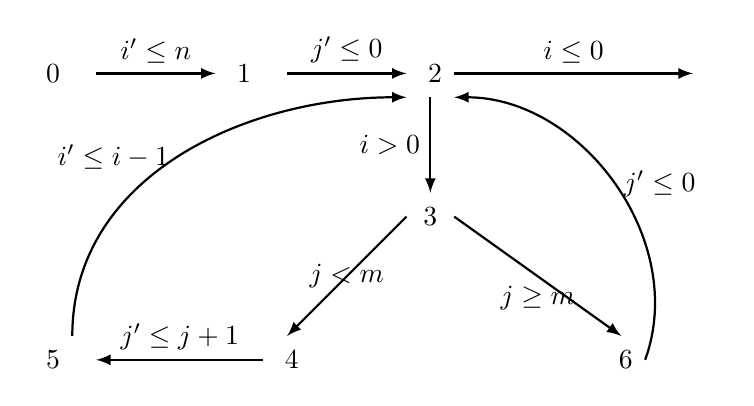
\begin{tikzpicture}[scale=\textwidth/20cm,samples=200]
  \draw[] (-8, 10) circle (0pt) node{{ $0$}};
  \draw[] (-4, 10) circle (0pt) node{{ $1$}};
  \draw[] (0, 10) circle (0pt) node{{ $2$}};
  \draw[] (0, 7) circle (0pt) node{{$3$}};
  \draw[] (-3, 4) circle (0pt) node{{ $4$}};
  \draw[] (-8, 4) circle (0pt) node{{ $5$}};
  \draw[] (4, 4) circle (0pt) node{{ $6$}};
  % Counter Variables
  \draw[] (6, 10) circle (0pt) node {\textbf{$\lex$}};
  %
  % Control Flow Edges:
  \draw[ thick, -latex] (-7, 10)  -- node [above] {$i' \leq n$}(-4.5, 10);
  \draw[ thick, -latex] (-3, 10)  -- node [above] {$j' \leq 0$}(-0.5, 10);
  \draw[ thick, -latex] (0, 9.5)  -- node [left] {$i > 0$} (0, 7.5) ;
  \draw[ thick, -latex] (0.5, 7)  -- node [below] {$ j \geq m $}  (4, 4.5);
  \draw[ thick, -latex] (-7.5, 4.5)  to  [out=90,in=180]  node [left] {$i' \leq i - 1$ }(-0.5, 9.5);
  \draw[ thick, -latex] (4.5, 4)  to  [out=70,in=0]   node [right] {$j' \leq 0 $}(0.5, 9.5);
  \draw[ thick, -latex]  (-0.5, 7) -- node  {$j < m$}  (-3, 4.5) ;
  \draw[ thick, -latex]  (-3.5, 4) -- node [above] {$j' \leq j + 1$}  (-7, 4) ;
  \draw[ thick, -latex] (0.5, 10)  -- node [above] {$i \leq 0$}  (5.5, 10);
  \end{tikzpicture}
  \caption{}
    \end{centering}
    \end{subfigure}
  \caption{
  (a) The Two Paths While Loop Example
    (b) The Abstract Execution Control Flow Graph}
      \label{fig:twoPathsWhile_abscfg}
  \end{figure}
  }
The program in Figure~\ref{fig:twoPathsWhile_abscfg}(a) is an example of two paths loop with different reachability-bounds on the control
locations in different paths.
Its abstract control flow graph is shown in Figure~\ref{fig:twoPathsWhile_abscfg}(b).
The edge $(0 \xrightarrow{i' \leq n} 1)$ on the top tells us the command 
$\clabel{\assign{i}{n}}^0$ is executed with a continuation point $1$, and the
command $\clabel{\assign{j}{0}}^1$ will be executed next.
The annotation $i' \leq 0$ is a difference constraint 
computed by $\absexpr$ over
the expression $n$ in the assignment command $\assign{i}{n}$.
It represents that the value of $i$ is less than or equal to value of $n$ after the
execution of $\clabel{\assign{i}{n}}^0$ and before executing $\clabel{\assign{j}{0}}^1$.
Another example constraint $i' \leq i - 1$ on the edge $5 \xrightarrow{i' \leq i - 1} 2$
describes the execution of
 the command at line $5$, 
$\clabel{\assign{i}{i - 1}}^{5}$. 
The $i'$ on the left side of $i' \leq i - 1$ represents the value of $i$ after the assignment operation,
and the right-hand side $i$ stores the value before the assignment.
The boolean constraint $i \leq 0 $ on the edge $2 \xrightarrow{i \leq 0} \lex$, 
represents the negation of the testing guard $i > 0$
in the $\ewhile$ command with loop header at line $2$.
$2 \xrightarrow{i \leq 0} \lex$ denotes that $i \leq 0$ must hold in order to perform this transition from program point $2$ to
the program exit. 
\end{example}
\section{Loop Refinement}
\label{sec:refine}
Three steps:
\begin{enumerate}
  \item It first collects all \emph{simple transition paths}.
  Every \emph{simple transition paths}, $\tpath \in \paths(\absG(c))$ 
  contains only the edges of atomic assignment or guard transitions without interleaving other paths.
  Each of them corresponds to a path in the flatten program in Definition~4.1 in \cite{GulwaniJK09}.
%
    \item \textbf{Rewrite the Program}
    Then it rewrites the program $c$ by rearranging all \emph{simple transition paths} as the syntax in \cite{GulwaniJK09} and preserves the same semantics.
\item \textbf{Refined Program}
Then it computes the 
refined program, $\rprog$ by Algorithm~1 in paper~\cite{GulwaniJK09}.
\\
This step invokes the algorithm REFINE from paper~\cite{GulwaniJK09} and compute the 
refined program $\rprog$ for a program $c$ given the rewritten program as input.
\end{enumerate}

\subsection{Collecting The Simple Transition Path}
We first collect the loop headers $\loopl(c) \subseteq \lvar(c)$ from a program $c$, which is the set of all program points corresponding to the loop headers in program $c$.
\begin{defn}[Loop Headers ($\loopl : \cdom \to \mathcal{P}(\ldom)$)]
  \label{def:loopl}
  \[
  \loopl(c) \triangleq 
  \left\{
    \begin{array}{ll}
      \{\}  & {c} = [{\assign x e}]^{l} \\
      \loopl({c_1}) \cup \loopl({{c_2}})  & {c} = {c_1};{c_2} \\
      \loopl(c_1) \cup \loopl({{c_2}})   & {c} =\eif([\bexpr]^{l}, c_1, c_2) \\
  \loopl(c') \cup \{l\}, &  {c}   = \ewhile ([\bexpr]^{l}, {c}')
  \end{array}
\right.
\]
  \end{defn}
% \begin{defn}[Loop Path]
%   \label{def:looppath}
% A simple transition path
% $\tpath \in \paths(\absG(c))$ for the program $c$, is a path on its abstract transition graph $\absG(c) = (\absV(c), \absE(c))$ with 
% \begin{itemize}
% \item a vertices sequence $(l_0, \ldots, l_n)$, where $l_i \in \absV(c)$ for every $i = 0, \ldots, n$ and
% %
% \item an edge sequence $(e_1, \ldots, e_n)$, where $e_i = (l_{i - 1}, dc_i, l_{i}) \in \absE(c)$ for every $i = 1, \ldots, n$,
% \end{itemize}
% %
% satisfying:
% \begin{itemize}
%   \item $l_i \neq l_j$ for every $i = 0, \ldots, n$ and $j = 0, \ldots, {n - 1}$,
%   \item $l_0$ is either the program point of a loop header or the program entrance ($l_0 = 0$),
%   i.e., $l_0 \in \loopl(c) \cup \{ 0 \}$
%   \item and $l_n$ is either the program point of a loop header or the program exit ($l_n = \lex$),
%   i.e., $l_0 \in \loopl(c) \cup \{ \lex \}$.
% \end{itemize}
% \end{defn}

\begin{defn}[Simple Tansition Path]
  \label{def:tpath}
A \emph{simple transition path}
$\tpath \in \paths(\absG(c))$ for the program $c$, is either a simple cyclic path, which has the same start- and end-point
or a simple path has either different while loop headers, the program entrance or exit as its start- and end-point
without visiting any loop header inside the path.
\\
Specifically, a path $l_0 \xrightarrow{dc_0} l_1 \xrightarrow{dc_1} \ldots l_n \in \paths(\absG(c))$ with the
vertices sequence $(l_0, \ldots, l_n)$, where $l_i \in \absV(c)$ for every $i = 0, \ldots, n$ and
%
the edge sequence $(e_1, \ldots, e_n)$, where $e_i = (l_{i - 1}, dc_i, l_{i}) \in \absE(c)$ for every $i = 1, \ldots, n$,
%
is a \emph{simple transition path} if and only if it satisfies,
\begin{itemize}
  \item $l_i \neq l_j$ for every $i = 0, \ldots, n$ and $j = 0, \ldots, {n - 1}$,
  \item $l_0$ is either the program point of a loop header or the program entrance ($l_0 = 0$),
  i.e., $l_0 \in \loopl(c) \cup \{ 0 \}$
  \item and $l_n$ is either the program point of a loop header or the program exit ($l_n = \lex$),
  i.e., $l_0 \in \loopl(c) \cup \{ \lex \}$,
  \item and $l_i \notin \loopl(c) \cup \{ 0, \lex \}$ for every $i = 1, \ldots, n-1$.
\end{itemize}
\end{defn}

\paragraph{Example.}
$2 \to 3 \to 6 \to 2$ is a transition path on $\absG(\kw{twoPathsWhile}(n, m))$ in Figure~\ref{fig:twoPathsWhile_abscfg}(b).
However, $2 \to 3 \to 6 \to 2 \to 3 \to 4 \to 5 \to 2$ is not a transition path because it is not simple (the program points $2$ and $3$ are visited twice).
In Figure~\ref{fig:threeWhile-overview}(b), $1 \to 2 \to 3 \to 4 \to 5 \to 6$ is not a transition path on $\absG(\kw{threeNestedWhile}(n, m, N))$ because it visits a loop header $3$ inside the path.

\subsection{Rewrite and Refine the Program}
\paragraph{Rewrite the Program}
\begin{algorithm}
  \caption{Program Rewriting $\kw{Rewrite}$}
  \label{alg:alg-refine_rewrite}
  \begin{algorithmic}[1]
    \REQUIRE program $c$
    \STATE finds all $c$'s \emph{simple transition path}s, $\tpath_1, \ldots, \tpath_n \in \paths(\absG(c))$.
    \STATE \textbf{init}: candidate set $W = \{c_1, \ldots, c_n\}$, where $c_i = \tpath_i$ and $i = 1, \ldots, n$
    \STATE \textbf{while} $W.size()> 1$:
    \STATE \quad create $c' = \rpchoose{c_1, \ldots, c_m}$ 
    s.t. $c_i \in W \land c_i[0] = c_j[0] \land c_i[-1] = c_j[-1], i, j = 1, \ldots, m$.
    \\ \quad $W.add(c')$ \qquad $W.remove(c_1, \ldots, c_m)$
    \STATE
    \quad create $c' = \rprepeat(c)$ s.t. $c_i \in W \land c[0] = c[-1] \land c[0] \in \loopl(c)$
    \\ \quad $W.add(c')$, \qquad $W.remove(c)$
    \STATE \quad create $c' = c_1; c_2$ s.t. $c_1, c_2 \in W \land c_1[-1] = c_2[0]$
    \\
    \quad $W.add(c')$ \qquad $W.remove(c_1, c_2)$
    \STATE \textbf{Endwhile}
    \\ $c^T = W[0]$
    \RETURN $c^T$.
\end{algorithmic}
\end{algorithm}
%
Line-2: initialize each candidate $c_i$ with a simple transition path $\tpath_i$.
\\
Line-4: for all the candidates $c_1, \ldots, c_m$ having the same starting and ending vertices, rewrite them into if statement as~\cite{GulwaniJK09}.
\\
Line-5: for every candidate $c'$, if it starts and ends with the same vertex, rewrite it into while loop statement as~\cite{GulwaniJK09}.
\\
Line-6: for every two candidates $c_1, c_2$, if $c_1$ ends with the same vertex as $c_2$'s starting label, rewrite them into sequence statement as~\cite{GulwaniJK09}.
\\
We use simple depth first search strategy computes all the \emph{simple transition path}s satisfying the Definition~\ref{def:tpath} below.
It guarantees that  every $\tpath$ is equivalent to a path $\rho$ in Definition~4.1 of \cite{GulwaniJK09}.

\paragraph{Refined Program}
We implement the algorithm REFINE from paper~\cite{GulwaniJK09} and compute the 
refined program $\rprog$ for a rewritten program $c$.

\section{Path-sensitive Reachability-Bound Analysis}
\label{sec:psrb}
Our path-sensitive reachability-bound algorithm relies on the \emph{Abstract Transition Graph}, $\absG(c)$, the \emph{Refined Program}, $\rprog$ and the upper bound invariant of the \emph{Ranking Function} computed previously for the program $c$.
It first requires to compute the new quantities, \emph{Path Reachability-bound} and the \emph{Loop Reachability-bound}, and this section introduces the definition and the following sections describe how we compute them.
%  of \emph{Path Reachability-bound} and the \emph{Loop Reachability-bound}. 

% Given a program $c$ with its \emph{Abstract Transition Graph}, $\absG(c)$ and refined program $\rprog$, our path-sensitive reachability-bound algorithm is presented as follows.

As pre-procedures, we first need to compute the loop bound, $BD(\rprog', c) \in \scexpr(c)$ for every subprogram $\rprog'$ of $c$ in $\rprog$, and use it to estimate the \emph{path local reachability-bound}, $\outinB(\rprog_l, \tpath, c) \in \scexpr(c)$ for each $\tpath$ w.r.t. the sub loop program $\rprog_l$.
\begin{defn}[Loop Bound]
  % \label{def:loopbound}
  For any program $c$ with it refined program $\rprog$,
  the loop bound $BD(\rprog', c) \in \scexpr(c)$ for a subprogram $\rprog'$ of $c$ in $\rprog$ is a upper bound on the iterating times of this program from its enter point to the exit point.
\end{defn}
% 
% Then we compute the \emph{path local reachability-bound}, $\outinB(\rprog_l, \tpath, c) \in \scexpr(c)$ for every sub loop program $\rprog_l$ of $c$ in $\rprog$.
\begin{defn}[Path Local Reachability-bound]
  % \label{def:pathlocalrb}
  Given program $c$ with its refined program $\rprog$ and a simple transition path $\tpath$ in this program, 
  let $l: \rprog_l = \kw{enclosed}(\rprog, \tpath)$ be a sub loop program in $\rprog$,
  then $\tpath$'s \emph{path local reachability-bound} w.r.t. $l: \rprog_l$,  $\outinB(\rprog_l, \tpath, c) \in \scexpr(c)$
  is an upper bound on the execution times of $\tpath$ when executing program $\rprog$.
\end{defn}
Intuitively,
% the local reachability-bound of a \emph{simple transition path},
$\outinB(\rprog_l, \tpath, c)$ bounds the execution times of $\tpath$ when executing its innermost loop program $\rprog_l$.
% and $\rprog$ is the closest loop where $\tpath$ is nested.
For example in the first interleaving pattern $\rprog_1^1$ in Example~\ref{ex:relatedNestedWhileOdd-overview}, 
$4:\rprepeat(\tpath_3)$ is the innermost loop program of $\tpath_3$. So we first compute $m - n$ as its \emph{path local reachability-bound} to bound its iteration times in its closest loop by Section~\ref{sec:pathlocalrb}.
% $4:\rprepeat(\tpath_3)$ is the innermost loop program of $\tpath_1$, $\tpath_2$ and $\tpath_4$.
% We compute the $\frac{m}{4}$ for all the three path $\tpath_1$, $\tpath_2$ and $\tpath_4$ w.r.t. $\rprog_1^1$, as their \emph{path local reachability-bound}.
% $\outinB(1: \rprog_1^1, \tpath_1) = \frac{m}{4}$,
% $\outinB(1: \rprog_1^1, \tpath_2) = \frac{m}{4}$,
% $\outinB(1: \rprog_1^1, \tpath_4) = \frac{m}{4}$,

Next, we define the \emph{loop reachability-bound},
$\lpchB(l: \rprog_l, \tpath, c) \in \scexpr(c)$ for every outer loop program $\rprog_l$ of $\tpath$ in $\rprog$. This quantity aims to precisely bound the iteration numbers of the outer loop $l$,
such that,
during these iterations, the innermost loop $l' = \kw{enclosed(\tpath)}$ is executed, i.e., reached.
\begin{defn}[Loop Reachability-bound]
% \label{def:looprb}
For a program with its refined program $\rprog$ and a simple transition path $\tpath$ in this program, 
let $l: \rprog_l$ be a loop program in $\rprog$,
then $l: \rprog_l$'s \emph{loop reachability-bound} w.r.t. $\tpath$,  $\lpchB(l: \rprog_l, \tpath, c) \in \scexpr(c)$
is the upper bound on iteration numbers of the outside loop $l$,
such that,
during these iterations, the nested loop $l' = \kw{enclosed(\tpath)}$ is entered.
\end{defn}
As introduced in Section~\ref{sec:overview} for Example~\ref{ex:relatedNestedWhileOdd-overview}, $\tpath_3$ has an outer loop program $\rprog_1^1$. Since $L_4$ will be ``entered'' only in the first iteration of $\rprog_1^1$,
we aim to compute $1$ for $\lpchB(\rprog_1^1, \tpath_3, c)$ in Section~\ref{sec:looprb}.
  % and we compute $\lpchB(\rprog_1^1, \tpath_3, c) = 1$. It is tight because the innermost loop of $\tpath_3$ will be ``entered'' only in the first iteration of $\rprog_1^1$.

% Intuitively $\lpchB(l: \rprog_l, \tpath, c) \in \scexpr(c)$
% is the bound on iteration numbers of the outside loop $l$,
% such that,
% during these iterations, the nested loop $l' = \kw{enclosed(\tpath)}$ is executed, i.e., reached.
The \emph{path reachability-bound}, $\inoutB(\rprog, \tpath)$ for each $\tpath$
aims to bound the execution times of $\tpath$ globally during the execution of $c$ and Section~\ref{sec:pathrb} presents the estimating algorithm.
%
\begin{defn}[Path Reachability-bound]
% \label{def:pathrb}
For a program $c$ with its refined program $\rprog$ and a simple transition path $\tpath$ in this program, 
$\tpath$'s reachability-bound, $\inoutB(\rprog, \tpath) \in \scexpr(c)$ is the upper bound on the
execution times of $\tpath$ when executing the $\rprog$.
\end{defn}
% Intuitively, $\inoutB(\rprog, \tpath)$ bounds the execution times of $\tpath$ globally during the execution of $c$.

For our running program in Example~\ref{ex:relatedNestedWhileOdd-overview}, since there isn't nested loop for $\tpath_1, \tpath_2$ and $\tpath_3$, we compute their $\inoutB(\rprog, \tpath) = \frac{m}{4} $, which is the same as their local bound.
While for $\tpath_3$ we compute  the $\inoutB(\rprog, \tpath_3) = \frac{m}{4} \times 1$ by multiplying its local bound with loop reachability bound.
% path is $\tpath_3 = \frac{m}{4} \times 1 = \frac{m}{4} $.

% \paragraph{Program Points Reachability-bound Computation}
% \label{sec:point-psrb}
The \emph{Reachability-bound} for program points is finally computed as follows.
For each program point in a program $c$, $l \in \lvar(c)$,
%  in a program $c$,
its \emph{reachability-bound}, $\psRB(c, l)$ during the execution of $c$ is computed as follows.
%
\begin{defn}[Program Point Reachability-bound Computation]
\label{def:point_psrb}
Given a program $c$ with its \emph{Abstract Transition Graph}, $\absG(c)$ and refined program $\rprog$,
the \emph{reachability bound} of each program point $l \in \lvar(c)$, $\psRB(c, l)$ 
sums up all the path reachability bounds, $\inoutB(\rprog, \tpath)$ over all simple transition paths $\tpath$ that contains the program point $l$.
\[ 
  \psRB(c, l) = 
  \sum
  \left\{ \inoutB(\rprog, \tpath) ~\vert~ \tpath \in \rprog \land 
  l \in \tpath \right\}\footnotemark
\]
$l \in \tpath$ denotes that the program point $l$ is a vertex on $\tpath$ 
and $\tpath \in \rprog$ denotes $\tpath$ is a simple transition path in $\absG(c)$.
\footnotetext{$l \in \tpath$ and $\tpath \in \rprog$, the $\in$ notation is abused to denote
the program point $l$ is a vertex on this path and $\tpath$ is a simple transition path on $\absG(c)$ respectively.}
\end{defn}
$\econfig{\psRB(c, l)}$ is a \emph{reachability-bound} for every program point $l$ in a program $c$.
\begin{thm}[Soundness of the Path-sensitive Reachability-bound Estimation]
\label{thm:pathsensitive_rb_soundness}
For every program ${c}$ and every label $l$ in this program,
$\econfig{\psRB(c, l)}$ is a \emph{Reachability-bound} for $l$ in $c$.
%
{\small
\[
  \begin{array}{l}
    \forall c, c_r \in \cdom, \tpath \in \absG(c), \trace_0 \in \ftdom_0(c),  \trace_r \in \ftdom_0(c_r), \trace \in \tdom, l, l' \in \ldom, \rprog \st 
    \\ \qquad
    \rprog = REFINE(\algrewrite(c))
    \land 
    \rprog = \algrewrite(c_r)
    \land
    \\ \qquad
    \land
    \Big(
    \config{c_r, \trace_0} \rightarrow^* \config{\clabel{\eskip}^{l'}, \trace_0 \tracecat \trace}
    \lor \config{c_r, \trace_0} \uparrow^{\infty} \trace_0 \tracecat \trace 
    \Big)
    \\ \qquad
    \implies \econfig{\psRB(c, l)}(\trace_0) \geq \counter(\trace, l)
  \end{array}.
\]
}
\end{thm}
  
\section{Loop Reachability Bound and Loop Bound Computation}
\label{sec:looprb}
The loop reachability bound is formally defined below. 

\begin{defn}[Loop Reachability Bound]
    \label{def:looprb}
    Loop Reachability Bound
    \begin{equation}
        \label{eq:looprb}
      \lpchB(l: \rprog, \tpath) \triangleq
        \frac{\lpinit(l: \rprog, \tpath) - \rffinal(\tpath)}{\lpnext(l: \rprog, \tpath)}
    \end{equation}
  \end{defn}

  We first compute each component in Equation.~\ref{eq:looprb}
  and solve the computation by SMT solver as follows.
  \\
  1. Compute the ranking function for every transition, $\locbound(\tpath)$ and estimate its maximum value,
  $\varinvar(\locbound(\tpath))$.
  This computation are adopted from \cite{sinn2017complexity} with more details in Section~\ref{sec:rank}.
  \\
  2. Compute the abstract states,  $\lpinit(l: \rprog, \tpath)$,
  $\rffinal(\rprog)$, and $\lpnext(l: \rprog, \tpath)$ using ranking function,
  as in Definition~\ref{def:alg-absstate}.
  \\
  3. Solve the equation using abstract states above and SMT solver.
%
\begin{defn}[Abstract States Computation]
\label{def:alg-absstate}
The abstract states $\lpinit(l: \rprog, \tpath)$, $\lpnext(l: \rprog, \tpath) \in \mathcal{A}_{in}$,
and $\rffinal(\rprog)$ are computed as follows.
\begin{itemize}
   \item 
The loop initial state 
$\lpinit(l: \rprog, \tpath) \in \mathcal{A}_{\lin}$ is symbolic expression as well. 
It describes the abstract initial value of $\tpath$'s ranking function before
any visit of $\tpath$ and during the first execution of $l: \rprog$.
\[
  \lpinit(l: \rprog, \tpath) \triangleq 
  \arg\max_{l_1}\left\{
       \varinvar(y) + v ~\middle\vert~ 
       \begin{array}{l} 
         (l_1, x' \leq y + v, l_2) \in \reset(x) 
         \\
         \land \absinit(\rprog) \leq l_1 \leq \absinit(\tpath)
       \end{array}
     \right\}
    , x = \locbound(\tpath)
  \]
\item
The loop next state 
$\lpnext(l: \rprog, \tpath) \in \mathcal{A}_{\lin}$ 
describes how much $\tpath$'s ranking function
is modified before
the second visit of $\tpath$ but during the second execution of $l: \rprog$.
\footnote{$l' \in \rprog$: the $\in$ notation is abused to denote
the program point $l'$ is a vertex on a path in the program $\rprog$.}
%
\[
  \begin{array}{l}
  \lpnext(l: \rprog, \tpath) \triangleq 
    \begin{array}{l}
  \sum\limits_{(x, \absevent) \in \inc(x) }
  \left\{ 
    \varinvar(y) + v ~\middle\vert~ \absevent = (l', x' \leq y + v, \_) \land  l' \in \rprog 
    \land l' \notin \tpath \right\}
    \\ \qquad 
    - \sum\limits_{(x, \absevent) \in \dec(x) }\left\{ 
      \varinvar(y) + v 
      ~\middle\vert~ \absevent = (l', x' \leq y + v, \_) \land l' \in \rprog \land l' \notin \tpath \right\}
    \end{array}
  \end{array}
  , x = \locbound(\tpath)
  \]
  \item  The \emph{Final State}, $\rffinal(\rprog)$ a conjunction of boolean expressions.
  It is the post-condition
  after the execution of $\rprog$.
\[
    \rffinal(\rprog) \triangleq 
    \bigwedge_{b \in \kw{Guard}(\rprog)}
    \neg b
\]
   $\kw{Guard}(\rprog)$ is the set of all the unique boolean expressions (i.e., the boolean constraints) on this program.
\end{itemize}
\end{defn}

\section{Ranking Function Computation and Estimation}
\label{sec:rank}
Three steps:
\begin{enumerate}
    \item It first collects three edge sets for each variable,
  in which the variable increases, decreases and reset respectively.
  \item
  Then, it assigns a symbol $x \in \scvardom$ to the edge on which this symbol decreases as this edge's ranking function.
  \item
  In the last step, it estimates the upper bound invariant on the maximum value of each ranking function recursively.
  In the meantime, it also computes a loop bound path-insensitivity for each loop, which can be used to compute the path reachability-bound later.
  \end{enumerate}

  The algorithm in this step is inspired from the Algorithm.2 in paper~\cite{SinnZV14},
  % which assigns a variable to each edge on which this variable decrease as its ranking function.
  the Algorithm.3 in paper~\cite{ZulegerGSV11},
  and the Definition.25 in Section 4 of paper~\cite{SinnZV17}.
  Algorithm.3 in paper~\cite{ZulegerGSV11} assigns a set of variables to each transition in which these variables decrease as the local bound
  and estimates the maximum value each variable in this set.
  Algorithm.2 in paper~\cite{SinnZV14} assigns a variable to each edge on which this variable decrease as its ranking function
  and then estimates the maximum value for the ranking function.
  The Definition.25 in paper~\cite{SinnZV17}
  assigns each transition with a variable that decreases in this transition, as the local bound and computes the bound similarly.
  %
  \subsection{Collecting Variable Modifications}
  For each variable $x$ in a program $c$, this step computes three edge sets, $\inc(x, c)$, $\dec(x, c)$,
  and $\reset(x, c)$ for $x$.
  Every edge in a set corresponds to a transition in which $x$ is increased,
  %  $\inc(x, c)$,
  decreased
  % $\dec(x, c)$ and 
  or reset
  % $\reset(x, c)$, 
  respectively.
  \\
  $\inc: \cdom \to \vardom \to \mathcal{P}(\absevent) $
  is the set of the edges where the variable increase, 
  %\\
  \[ \inc(x, c) = \left\{ \absevent | \absevent = (l, x' \leq x + v, l') \land \absevent \in \absflow(c) \right\} \]
  %\\
  $\dec: \vardom \to \mathcal{P}(\absevent) $
  is the set of abstract events where the variable decrease,
  %\\
  \[\dec(x, c) = \left\{\absevent| \absevent = (l,  x' \leq x - v, l') \land \absevent \in \absflow(c) \right\}\]
  %\\
  $\reset: \cdom \to \vardom \to \mathcal{P}(\absevent) $ is the set of the abstract events where the variable is reset,
%
  \[\reset(x, c) = \left\{ \absevent| \absevent = (l,  x' \leq y - v, l') \land x \neq y \land \absevent \in \absflow(c) \right\}\]
  Additionally,
  we also compute the reset graph $\resetG(c)$ and the reset chain, $\resetchain(x, c) \in \mathcal{P}(\mathcal{P}(\absevent))$ for every rank $x$.
  The $\resetchain(x, c)$ for every rank $x$ contains all the paths in $\resetG(c)$ that are end at $x$.
  The computation of $\resetG(c)$ and $\resetchain(x, c)$ follows the Definition~20 in~\cite{SinnZV17}.
  \[\resetG(c) = (\resetV(c), \resetE(c))\]
  \[\resetE(c) = \left\{ (x, \absevent, y) ~\vert~ \absevent \in \reset(x, c) \land \absevent = (l, x' \leq y + c, l') \right\} \]
  \[\resetV(c) = \left\{ x ~\vert~ (x, \_, \_) \in \resetE(c) \lor (\_, \_, x) \in \resetE(c) \right\} \]
  In a variable $x$'s reset chain set, $\resetchain(x, c)$, in each chain $(e_0, \ldots, e_m) \in \resetchain(x, c)$
  a variable $x_i$ is reset by another variable $x_{i + 1}$ on edge $e_{i}$
  and $x_{i + 1}$ is reset on edge $e_{i + 1}$ recursively
  for every $i = 0, \ldots, m - 1$.
  $x$ is reset on the first edge $e_0$ of every sequence in $\resetchain(x, c)$.
  {Each edge $e_i$ in a sequence $(e_0, \ldots, e_m) \in \resetchain(x, c)$
  resets a variable $x_i$ by another variable $x_{i + 1}$ such that $x_{i + 1}$
  is reset on edge $e_{i + 1}$ recursively. The first edge $e_0$ of each sequence resets the variable $x$.}
  % 
  \\
  In the following steps, $c$ is omitted in $\inc(x, c)$,
  $\dec(x, c)$ and $\reset(x, c)$ for concise when the reference of a program $c$ is clear in the context.

  \subsection{Assigning The Ranking Function to An Edge}
  For each edge in the transition graph $\absG(c)$ of a program $c$,
  this step assigns the variable that decreases on this edge as the ranking function of this edge.
  This step adopts the local bound computation method in Section 4 of~\cite{SinnZV17} to assign the local bound to each edge,
  formally as follows.
  \begin{defn}[Ranking Function Generatation]
  \label{def:ranking_gen}
  For every edge $\absevent$ in the transition graph $\absG(c)$ of a program $c$,
  its \emph{ranking function/local bound}, $\locbound(\absevent, c)$
  is the variable that decreases on this edge, computed as follows,
  %
  \[ 
\begin{array}{ll}
  \locbound(\absevent, c) \triangleq 1 
  & \absevent \notin SCC(\absG(c))
  \\
  \locbound(\absevent, c) \triangleq x
  & \absevent \in SCC(\absG(c)) \land \absevent \in \dec(x, c) \land  \absevent = (\_, \_ , x' \leq x - v) \\
  \locbound(\absevent, c) \triangleq x
  & \exists \absevent' \in \absG(c), \tpath \in \paths( \absG(c)) \st \absevent, \absevent' \in \tpath \land \locbound(\absevent', c) = x \\
  % \in SCC(\absG(c)) \land \absevent \in \dec(x, c) \land  \absevent = (\_, \_ , x' \leq x - v) \\
  \locbound(\absevent, c) \triangleq x
  & \absevent \in SCC(\absG(c)) \land 
  \absevent  \notin \bigcup_{x \in \vardom} \dec(x, c)
  \land \absevent \notin SCC(\absG(c) \setminus \dec(x, c))\\
  \locbound(\absevent, c) \triangleq \infty
  & o.w..
\end{array}
\]
  $SCC(\absG(c))$ is the set of all the strong connected components of $\absG(c)$.
  \end{defn}
    The first case is straightforward. 
    For the label $l$ which is not in any while loop, 
    the labeled command with the label $l$ will be 
    evaluated at most once. 
    The second and third cases are guaranteed by the \emph{Discussion on Soundness} in Section 4 in~\cite{SinnZV17}.
    The soundness is formalized in Lemma~\ref{lem:local_bound_sound} with proof in Appendix~\ref{apdx:pathinsensitive_rb_soundness}.
  %
  \paragraph{Example}
  In Figure~\ref{fig:relatedNestedWhileOdd-overview}(b), we assign variable $i$ to edge $7 \xrightarrow{i' \leq i - 1} 1$ as ranking.
  If we remove this edge, the edges on $\tpath_2$ and $\tpath_1$ are not in any SCC, so they also have the same ranking.
In the same way, ranking for edges on $\tpath_4$ is $i$ as well and $k$ for them on $\tpath_3$.


  \subsection{Ranking Function Estimation}
  This step estimates the upper bound, $\varinvar(x, c) \in \scexpr(c)$
  on the maximum value for each ranking function  $x \in  \vardom \cup \scvar(c)$.
  \\
  For a program $c$, the \emph{ranking function bound},
  $\varinvar(\locbound(\absevent, c), c)$ is 
  the bound on the maximum value of the ranking function  
  assigned to the edge $\absevent \in \absE(c)$, formally in Definition~\ref{def:ranking_bound}.
  \\
  In order to estimate the maximum value of $\locbound(\absevent, c)$ assigned to edge $\absevent \in \absE(c)$,
  the bound on the iteration times of each corresponding edge, $\absclr(\absevent, c)$ 
  is computed interactively in a path-insensitive manner.
  % \\ 
  % $\varinvar (x, c) \in \scexpr(c)$
  % \\
  % $\absclr(\absevent, c) \in \scexpr(c)$
  \begin{defn}[Ranking Function Estimation]
    \label{def:ranking_bound}
  For a program $c$ and an edge $\absevent \in \absE(c)$,
  the \emph{ranking function bound}, 
  $\varinvar(\locbound(\absevent, c), c)$ for the ranking function $x = \locbound(\absevent, c)$
  of this edge
  is computed as follows,
    \[ 
  \begin{array}{lll}
    \varinvar(x, c) & \triangleq x & x \in \scvar(c) \\
    \varinvar(x, c) & \triangleq \incrs(x, c) + \max\left\{\varinvar(y, c) + v ~\mid~ (l, x' \leq y + v, l') \in \reset(x, c) \right\} & x \notin \scvar(c)
  \end{array}
  \]
  %
  where $\incrs(x, c) \triangleq \sum\limits_{\absevent \in \inc(x, c)}\{\absclr(\absevent, c) \times v ~\mid~ \absevent = (l, x' \leq x + v, l')\}$
  The path-insensitive bound, $\absclr(\absevent, c) \in \scexpr(c)$  on the execution times of the transition $\absevent$, is interactively computed as well as below,
\[ 
\begin{array}{lll}
  \absclr(\absevent, c) 
  & \triangleq \varinvar(\locbound(\absevent, c), c)  &  \\
  & \quad \text{if} ~ \locbound(\absevent, c) \in \scvar(c) & \\
  \absclr(\absevent, c) 
  & \triangleq
    \sum \left\{ \incrs(y, c) | ch \in \resetchain(x, c) \land y \in ch \right\} & \\
    & \quad + 
  \sum\limits_{ch \in \resetchain(x, c)}
  \min \left\{\absclr(\absevent', c) ~\mid~ \absevent' \in ch\right\} \times 
  \big(\varinvar(in(ch), c) 
  + \sum\limits_{(\_, (\_, x' \leq y + v, \_), \_) \in ch} v \big) & \\
  &  \quad \text{if} ~\locbound(\absevent, c) = x \land x \notin \scvar(c) & ,
\end{array}
  \]
 where $in(ch)$ is the first vertex of the reset chain $ch$.
\end{defn}
  %
We also have the soundness of this path-insensitive transition bound. For a program $c$ and an edge $\absevent \in \absE(c)$,
$\absclr(\absevent)$ is a sound upper bound
on the execution times of this transition by paper~\cite{SinnZV17}, formally below in Theorem~\ref{thm:pathinsensitive_rb_soundness} with proof in Appendix~\ref{apdx:pathinsensitive_rb_soundness}.
%
\begin{thm}[Soundness of the Path-insensitive Transition Bound]
  \label{thm:pathinsensitive_rb_soundness}
For each program ${c}$ and an edge $\absevent = (l, \_, \_) \in \absG(c)$, if $l$ is the label of an assignment command,
%  label $l \in \lvar(c)$,
then its \emph{path-insensitive transition bound} $\absclr(\absevent, c)$ 
 is a sound upper bound on 
the execution times of this assignment command in $c$.
  \[
    \begin{array}{l}
      \forall \trace_0 \in \ftdom_0(c), \trace \in \tdom, c \in \cdom, l, l' \in \lvar(c) \st
      \Big( \config{c, \trace_0} \rightarrow^{*} \config{\clabel{\eskip}^{l'}, \trace_0 \tracecat \trace} 
        \lor  \config{c, \trace_0} \uparrow^{\infty} \trace_0 \tracecat \trace \Big)
       \\ \qquad \qquad
       \implies
       \exists \absevent = (\_, l, \_) \in \absflow(c) \land
      \counter(\trace, l) \leq \econfig{\absclr(\absevent, c)}(\trace_0)
    \end{array}
  \]
\end{thm}
%
\paragraph[example]{Example.}
% \todo{The w example}
Using this ranking function based approach, we first find the ranks for every transition,
$\locbound(0 \to 1) = 1$,
$\locbound(1 \to \lex) = 1$,
$\locbound(1 \to 2) = i$,
$\locbound(2 \to 3) = i$,
$\locbound(3 \to 4) = i$,
$\locbound(4 \to 5) = k$,
$\locbound(5 \to 4) = k$,
$\locbound(4\to 6) = \locbound(6 \to 7) = \locbound(7 \to 1) = i$,
and $\locbound(2 \to 8) = \locbound(8 \to 1) = i$,
Then we estimate the upper bound invariant for the ranking function $i$ and $k$ by computing the transition bound in the same time.
We get $\varinvar(i, c) = n$ and $\varinvar(k, c) = m$.
While the transition bound for each transition is the same as the upper bound invariant of its ranking function.
They are loose and path-insensitive. 

Specifically, in Example~\ref{ex:relatedNestedWhileOdd-overview}, the ranking $i$ is reset by $n$ at edge $0 \to 1$ and 
$k + m$ at edge $6 \to 7$ and $k$ is assigned value $i - m$ at edge $3 \to 4$. Through reset chain graph (which we do not fully presented but can be found in the Definition~20 in~\cite{SinnZV17}), we estimate a symbolic value $n$ for both ranking variable $i$ and $k$.
Interactively, iteration bounds for all the edges in this loop are $n$ as well path-insensitively.
\section{Reachability Bound Computation}
\label{sec:alg-rb}
\subsection{Path Global Reachability-Bound}
\label{sec:pathrb}
We first compute $\kw{enclosing}(\rprog)$, which is the set containing \text{all the loops $l:\rprog$ which are nested inside } $\rprog$.
\\
Then, the path global reachability-bound, $\inoutB(\rprog, \tpath)$ for a \emph{simple transition path} $\tpath$ is computed as in Definition~\ref{def:pathrb}.
%
\begin{defn}[Path Reachability-Bound]
  \label{def:pathrb}
\[
  \begin{array}{rcl}
    \inoutB(\tpath, \tpath) & \triangleq & 1  \\
    \inoutB(\tpath', \tpath) & \triangleq & \highlight{0} \qquad \text{if } \tpath' \neq \tpath\\
    \inoutB(\rprog_1;\rprog_2, \tpath) & \triangleq & \inoutB(\rprog_1, \tpath) + \inoutB(\rprog_2, \tpath) \\
    \inoutB(l: \rprog', \tpath) & \triangleq & 
    \highlight{\outinB(\rprog', \tpath), \qquad \text{if } l = \kw{enclosed}(\tpath)}
    \\
    &  \triangleq & 
   0, \qquad \qquad \qquad \quad ~~ \text{if }  \kw{enclosed}(\tpath) \notin \kw{enclosing}(\rprog')
    \\
    &  \triangleq & 
    \highlight{
      \lpchB(l:\rprog', \tpath ) }
    \highlight{\times \max\limits_{l = \kw{enclosed}(l':\rprog'')}
   \{\inoutB(l':\rprog'', \tpath)\} } \footnotemark, o.w. \\
    \inoutB(\rpchoose{\rprog_1, \ldots, \rprog_m }, \tpath) & \triangleq 
    & \max\left\{ \inoutB(\rprog_1, \tpath), \ldots, \inoutB(\rprog_m, \tpath) \right\} 
    \\
    \inoutB(\rprepeat(\rprog'), \tpath) & \triangleq & \outinB(\rprepeat(\rprog'), \rprog) \times \inoutB(\rprog', \tpath)\\
    &  & \text{this case will never be matched}
    \end{array}
  \]
  \end{defn}
\footnotetext{There is only one non-zero $\inoutB(l':\rprog'', \tpath)$ where $\tpath \in \rprog''$, all the others $\inoutB(l':\rprog'', \tpath)$ where $\tpath \notin \rprog''$ equal to $0$}%
We show that $\inoutB(\rprog, \tpath)$ bounds the execution times of $\tpath$ during the execution of $\rprog$

We show the \emph{path reachability-bound} of the simple transition path $\tpath$ in a refined program $\rprog$ is a sound upper bound of its execution times when executing the program in Lemma~\ref{lem:pathrb-sound}, with the proof in \highlight{Appendix~\ref{apdx:pathrb-sound}}.
\begin{lem}[Soundness of the Path Reachability-Bound]
  \label{lem:pathrb-sound}
  For any program with its refined program $\rprog$ and a simple transition path $\tpath$ in this program,
  the execution times of $\tpath$ when executing the $\rprog$ is bounded by $\inoutB(\rprog, \tpath)$.
  \[
    \begin{array}{l}
    \forall c \in \cdom, \tpath \in \absG(c), \trace_0 \in \tdom_0(c), \trace \in \tdom, \rprog \st 
    \rprog = REFINE(c)
    \land
    \config{c, \trace_0} \to^* 
    \config{{\eskip, \trace_0 \tracecat \trace}}
    \\ \qquad
    \implies
    \config{\inoutB(\rprog, \tpath)}(\trace_0) \geq \counter(\vtrace, L(\tpath)).
    \end{array}
    \]
  \end{lem}

\subsection{Program Points Path-sensitive Reachability-Bound}
\label{sec:point-psrb}
For each program point in a program $c$, $l \in \lvar(c)$,
%  in a program $c$,
its \emph{path-sensitive reachability-bound}, $\psRB(c, l)$ is a sound upper bound on the executing times of $l$ during the execution of $c$.
%
 \begin{defn}[Path-Sensitive Reachability Bound]
  \label{def:point_psrb}
  Given a program $c$ with its \emph{Abstract Transition Graph}, $\absG(c)$ and refined program $\rprog$,
  the \emph{reachability bound} of each program point $l \in \lvar(c)$, $\psRB(c, l)$ 
  sums up all the path reachability bounds, $\inoutB(\rprog, \tpath)$ over the $\tpath$ which contains the program point $l$.
  \[ 
    \psRB(c, l) = 
    \sum\limits_{\tpath \in \rprog \land 
  l \in \tpath} 
  \inoutB(\rprog, \tpath)
  \]
  $l \in \tpath$ denotes that the program point $l$ is a vertex on $\tpath$ 
  and $\tpath \in \rprog$ denotes $\tpath$ is a simple transition path of program $c$.
 \end{defn}
We show that $\config{\psRB(c, l)}$ is a \emph{Reachability-Bound} for every program point $l$ in a program $c$ with proof in Appendix~\ref{apdx:psrb-sound}.
\begin{thm}[Soundness of the Path-sensitive Reachability Bound Estimation]
    \label{thm:pathsensitive_rb_soundness}
  For every program ${c}$ and every label $l$ in this program,
  $\config{\psRB(c, l)}$ is a \emph{Reachability-Bound} for $l$ in $c$.
  %
  \[
    \forall c \in \cdom, \trace_0 \in \tdom_0(c), \trace \in \tdom \st 
    \config{{c}, \trace} \to^{*} \config{\eskip, \trace_0 \tracecat \vtrace} 
    \implies \config{\psRB(c, l)}(\trace_0) \geq \counter(\vtrace, l) 
    \]
  \end{thm}



\section{Informal Discussion on Soundness and Path-sensitivity}
\label{sec:thminformal}
\subsection{Loop Bound}

\subsubsection{Soundness}
We present two ways for computing a loop bound on a single while loop path, both of them are sound.

\highlight{\textbf{Loop Bound Soundness Discussion - 1}}
The second on in Equation.~\ref{eq:absBD} relies on the soundness of the $\absclr(\absevent, c)$
in Definition~\ref{def:ranking_bound} in Section~\ref{sec:rank}.
For a program $c$ and an edge $\absevent \in \absE(c)$, $\absclr(\absevent, c)$ is a sound upper bound on the execution times of this transition,
formally in Theorem~\ref{thm:pathinsensitive_rb_soundness}. 
Proof of this theorem is in Appendix~\ref{apdx:pathinsensitive_rb_soundness}.

\highlight{\textbf{Loop Bound Soundness Discussion - 2}}
The first computation method in Section~\ref{sec:looprb} is based on the in Definition~\ref{def:loopbound} and also relies on external SMT solver.
For every transition path $\rprog$, the $BD(\rprog)$
is a sound upper bound on its execution times locally.
\\
This bound is sound locally by assuming
that all the loops and transition paths where $\rprog$ is nested execute only once.
This assumption comes from the computation of the $\varGD$ and the depth first search strategy.
\\
For every base case, i.e., a simple transition path, 
$\varGD(\rprog) =  \rfinit(\tpath) - \rfnext(\rprog)$
counts the variables' changes only once. In this way, it assumes all the outside patterns and loops execution only once.
In the other two cases,  $\varGD(\rprepeat(\rprog))$ and $\varGD(\rpseq(\rprog_1, \rprog_2))$
has the same assumption when compute the variables' changes.
The soundness also relies on the operation $\frac{\rfinit(\rprog) - \rffinal(\rprog)}{\varGD(\rprog)}$,
which can be solved by external SMT solver,
or solved by Definition~\ref{def:ranking_bound} in Section~\ref{sec:rank}.
%
\begin{thm}[Soundness of Loop Bound]
\label{thm:sound_outsidein}
For every program $c$ with it refined program $\rprog$,
if $\rprog$ is a transition path of this program, then the $BD(\rprog)$
is a sound local bound on the execution times of $\rprog$ in program $c$.
\[
    \begin{array}{l}
    \forall c \in \cdom, \rprog, \rprog, \trace_0 \in \tdom_0(\rprog), \trace_1, \trace \in \tdom \st 
    \rprog \in \rprog \land
    \rprog = Alg.4(c)
    \\ \qquad
    \land
    \config{c, \trace_0} \to^* \config{\highlight{\ewhile (\rprog, \cdots)}, \trace_0 \tracecat \trace_1} 
    \land 
    \config{\rprog, \trace_0 \tracecat \trace_1} \to^* \config{{\eskip, \trace_0 \tracecat \trace_1 \tracecat \trace}}
    \\ \qquad
    \implies {\vcounter(\trace, L(\rprog))} \leq BD(\rprog)(\trace_0 \tracecat \trace_1).
    \end{array}
\]
\end{thm}
\highlight{Informal Discussion}
\\
Theorem~\ref{thm:sound_outsidein} guarantees that
the bound for every transition path $\rprog$, the $BD(\rprog)$
is a sound upper bound on its execution times, by assuming
that all the loops and transition paths where $\rprog$ is nested execute only once.
\\
In paper \cite{sinn2017complexity} Definition~9, they informally discussed the local bound soundness.
$v$ is a local bound if it has the same decreasing time as the transition's execution time.
By assuming that certain program parts (those were e increases) are not executed,
then value of $v$ can limit the execution time of that transition.
\\
In our soundness, we assume all the code pieces not inside this transition path are executed at most once (once if they show up in front of the program
zero time if not).
In this case, this bound limits the execution time of this transition path.

\subsubsection{Path-sensitivity}
$BD(\rprepeat({\rprog}))$  is path-insensitive because we only compute the loop bound
for the single loop path in a refined program $\rprog$.
But our alternative computation method in Section~\ref{sec:looprb} has a better performance in the following sense.

\highlight{
  \textbf{Improvement Discussion:}
\\
The computation of $BD(\rprepeat({\rprog}))$ 
as below is more efficient and accurate than existing techniques.
\\
The method $T(c, l)$ in \cite{GulwaniJK09} can also compute a
bound on the iteration numbers of $\rprepeat({\rprog})$ locally based on
the same semantics and syntax.
Specifically, $T(c, l)$ call the $\kw{BOUNDFINDERD}$ function as follows:
\\
$\kw{BOUNDFINDERD(INITD(c, l_0, \absinit(\rprepeat({\rprog}))),
NEXTD(c, l_0, \absinit(\rprepeat({\rprog})), V_{\lin} )}$.
However, the $\kw{BOUNDFINDERD}$ function in \cite{GulwaniJK09} relies an arbitrary interface to
compute the bound on the iteration numbers.
The efficiency and accuracy of this computation fully depend on this arbitrary interface.
\\
In comparison to them, the alternative loop bound computation method in 
Definition~\ref{def:loopbound} based on the abstract transition graph $\absG(c)$ is more accurate.
}

\subsection{Path Local Reachability Bound}
\subsubsection{Path-sensitivity}
\highlight{
  The computation
  filters out the execution of other transition paths that are nested in the same loop as $\tpath$.
  In this way, the following repeat chain bound computations are path-sensitive
  because they only deal with $\tpath$'s execution over this chain.
  }
  \highlight{\textbf{The Path-sensitivity Discussion Informally}}
  \\
  For every multiple-paths loop,
  this bound computes the bound for every simple transition path path-sensitively.
  In comparison to the traditional bound computation methods, they
  estimate the bound of different paths by taking maximum overall paths.
  \\
  The path-sensitivity is guaranteed by the following informal discussion.
  \\
  If a simple transition path isn't nested in any $\rprepeat$ annotation, then
  $\outinB(\tpath) = 1$ is sound and tight because it bounds one execution of the while body accurate.
  \\
  If a simple transition path is nested in some $\rprepeat$ annotations,
  $\rpch(l: \rprog, \tpath) \triangleq \rprog_m \to \rprog_{n-1} \to \cdots \to \rprog_{0} \to \tpath$, we have the following guarantees.
  \\
  1. $\rprog_n$ is a unique transition path of this loop,
  and isn't a sub-pattern of any other transition paths in this loop.
  \\
  2. for every $i = n, \cdots, 0$, $\outinB(\rprog_{i - 1})$ bounds the execution time of $\rprog_{i - 1}$ with the assumption that $\rprog_{i}$ executes only once.
  \\
  3. $\tpath$ only shows up once inside $\rprog_n$.
  \\
  By 1. 2. 3. guarantees, multiplication of $\outinB(\rprog_{i - 1})$ for every $i = n, \cdots, 0$ is the accurate execution time of this
  simple transition path in the transition path $\rprog_n$.
  \\
  In the case that loop has multiple transition paths, $\rpchoose{l: \rprog_1, \cdots, l: \rprog_n}$,
  \\
  We first find every repeat chain of this loop for this simple transition path.
  Then we compute the execution time of $\tpath$ on every repeat chain and take the maximum value.

\subsubsection{Soundness}
\emph{Soundness}
    \\
    \emph{Path Local Reachability Bound}  $\outinB(\rprog, \tpath)$.
    For a simple transition path $\tpath$ with its closest enclosing while loop at $l$ in a program $\rprog$, 
    $\outinB(\rprog, \tpath)$
    is a sound bound on its execution times in side $l$.
    \\
    For a simple transition path $\tpath$ only enclosed by one transition path $\rprepeat(\tpath)$, 
    we know $\outinB(\rprog, \tpath) = \outinB(\rprepeat(\tpath), \rprog)$.
    Since $\outinB(\rprepeat(\tpath), \rprog)$ is a sound local bound on the iteration times
    of $\rprepeat(\tpath)$ by assuming all the outside loops executes only once.
    In this sense, $\outinB(\rprepeat(\tpath), \rprog)$ is also a sound bound on the iteration times globally.
    \\
    For a simple transition path $\tpath$ nested in multiple transition paths $\rprog_1, \cdots, \rprog_m$,
    we know $\outinB(\rprog, \tpath) = \prod\limits_{i = 1, \cdots, m}\outinB(\rprog_i, \rprog)$.
    By the same guarantee from $\outinB(\rprog_i, \rprog)$, it is sound to multiply each of them.
    
  %  


\subsection{Loop Reachability Bound}
\subsubsection{Path-sensitivity}
$\lpchB(l: \rprog, \tpath) \in \mathcal{A}_{\lin}$.
\\
For every simple transition path $\tpath$
and a loop whose header is at program point $l$ in a refined program $\rprog$,
 $\lpchB(l: \rprog, \tpath) \in \mathcal{A}_{\lin}$ computes a symbolic expression in $\mathcal{A}_{\lin}$
as the \emph{Relative Loop Bound} for the $\tpath$ and loop $l$.
\\
It bounds the iteration numbers of the loop $l$ w.r.t.
the inner loop $l'$ that is $\tpath$'s closest enclosing loop,
such that,
% the simple transition path $\tpath$.
% This $\tpath$'s closest enclosing loop has the loop header at $l'$ and $l'$ is nested inside the loop $l$.
% \\
% It estimates the iteration numbers of loop $l$ such that 
during these iterations of loop $l$, the nested loop $l'$ is executed.
\highlight{
% the for every program control location,
% how many times the innermost loop of this control location will be touched w.r.t. every
% outside loop it is nested in.
This is distinguished from the traditional methods, which only compute the bound on the iteration number
for the inner loop w.r.t one iteration of the outside loop where it is nested.
\emph{Relative Loop Bound} for $\tpath$ and $l$ bounds the number of the iterations for
the outside loop $l$,
% w.r.t. an inner loop.
%  of every control location.
such that during these iterations of the outside loop $l$, the inner loop $l'$ is entered. 
}

\highlight{
  \emph{Improvements}
  \\
  $\lpinit(l, \tpath)$, and $\lpnext(l, \tpath)$ can be computed using the 
  $\kw{INIT}(c, i, \absinit(\tpath))$ and $\kw{NEXT}(c, i, \absinit(\tpath))$ from paper \cite{GulwaniJK09}.
  % \\
Then, based on the same semantics and syntax,
the $\lpchB(l, \tpath)$ can be computed as
\\
$I(l, l') = \kw{BOUNDFINDERD(INIT(c, i, \absinit(\tpath)), NEXT(c, i, \absinit(\tpath)), V_{\ln})}$.
% from paper \cite{GulwaniJK09}.
\\
There are two improvements comparing to their method.
\\
1. $I(l, l')$ is the bound on iteration numbers of the inner loop $l'$ in each iteration of outside loop.
This is equivalent to the OutIn bound of $l'$ if $l$ is the closest enclosing loop of $l'$.
By multiplying $I(l, l')$ with $\outinB(l')$
 they assume $l'$ is executed in every $l$'s iteration.
 In this sense, they over-approximate the iteration numbers of the inner loop $l'$.
 \\
2. However, $\kw{BOUNDFINDERD}$ in paper~\cite{GulwaniJK09} is an arbitrary interface computing the bound on iteration numbers of $l$
separately.
The efficiency and accuracy of their algorithm fully depend on this arbitrary interface.
\\
In comparison to them, the computation method in Definition~\ref{def:looprb} based the
ranking functions and abstract states over the abstract transition graph $\absG(c)$ is more accurate.
 }

\subsubsection{Soundness}

\emph{Soundness}
\\
\emph{Relative-Loop Bound} $\lpchB(l: \rprog, \tpath)$. In a refined program $\rprog$,
for its every loop at the program point $l$ and a transition path $\tpath$ inside this loop,
the \emph{Relative Loop Bound} $\lpchB(l: \rprog, \tpath)$ is a symbolic bound
on the number of $l$'s iteration numbers,
%  will 
% bound the execution times of $L_{t_0}$
% in each single execution of the $L_{t_i}$ for every
such that during these iterations, the closest loop $l'$ enclosing $\tpath$ will be executed.
\\
The soundness is guaranteed by the operation
 $\frac{\lpinit(\rprog, \tpath) - \rffinal(\rprog, \tpath)}{\lpinit(\rprog, \tpath) - \lpnext(\rprog, \tpath)}$.
 In this operation, $\lpnext(\rprog, \tpath)$ computes the variables states of the $\tpath$
after visited the program point $l$ the second time and before visiting any other program point.
% it is 
In the same time, the soundness also relies on an external solver. 



\subsection{Path Reachability Bound}
\subsubsection{Path-sensitivity}
\subsubsection{Soundness}


\emph{Soundness} of the \emph{Path Reachability Bound}  
For every simple transition path $\tpath$, the $\inoutB(\tpath, \rprog)$
is a sound upper bound on its execution times globally.
\\
In every base case, a simple transition path not nested in any loop, or just inside one loop.
Then $\inoutB(\tpath, \rprog) = \outinB(\rprog, \tpath)$, which is the bound on its execution times without considering
outside loops' executions. Since there isn't any outside loop, this operation is sound.
In the same time, the soundness is guaranteed by the $\outinB(\rprog, \tpath)$.
\\
For every simple transition path nested in multiple loops, if $l$ is the closest loop $\tpath$ comes from, then
$\inoutB(\tpath, \rprog) =
\prod\limits_{l' \in \lpch(\tpath, \rprog)} \rpchB(l', \tpath, \rprog) \times \outinB(\rprog, \tpath)$.
Since $\lpchB(l', \tpath, \rprog)$ bounds the number of $l'$'s iteration numbers,
%  will 
% bound the execution times of $L_{t_0}$
% in each single execution of the $L_{t_i}$ for every
such that during these iterations, the $\tpath$ will be executed,
it is sound to multiply these bounds by $\outinB(\rprog, \tpath)$.
In the same time, the soundness also relies on the soundness of $\outinB(\rprog, \tpath)$ and $\rpchB(l', \tpath, \rprog)$. 
% Since 
% In this way, it assumes all the outside patterns and loop execution only once.
% In the other two cases,  $\varGD(\rprog, \rprepeat(\rprog))$ and $\varGD(\rprog, \rpseq(\rprog_1, \rprog_2))$
% has the same assumption.
% \todo{reference}
% \end{itemize}
%
\begin{thm}[Soundness of Path Reachability Bound]
  \label{thm:sound_path-rb}
  For every program $c$ with it refined program $\rprog$ and 
  every simple transition path $\tpath$ in this program,
   the $\inoutB(\tpath, \rprog)$
is a sound bound on the execution times of $\tpath$ in $c$.
  \[
    \begin{array}{l}
    \forall c \in \cdom, \tpath \in \absG(c), \trace_0 \in \tdom_0(c), \trace \in \tdom, \rprog \st 
    % \rprog \in \rprog \land
    \rprog = Alg.4(c)
    % \\ \qquad
    \land
    \config{c, \trace_0} \to^* 
    % \config{\highlight{\tpath; \rprog', \trace_0 \tracecat \trace_1} 
    % \land 
    % \config{\rprog, \trace_0 \tracecat \trace_1} \to^* 
    \config{{\eskip, \trace_0 \tracecat \trace}}
    \\ \qquad
    \implies
    \vcounter(\trace, L(\tpath)) \leq \inoutB(\tpath, \rprog)(\trace_0).
    \end{array}
    \]
\end{thm}
\todo{Formalize the Proof}
\\
Theorem~\ref{thm:sound_path-rb} guarantees that
for every simple transition path $\tpath$ in a program $c$ with its refined program $\rprog$,
the $\inoutB(\tpath, \rprog)$
is a sound upper bound on its execution times in $c$.


% \cleardoublepage
% \section{Path-sensitive Reachability-Bound Computation}
% \label{sec:inoutalg}
% \textbf{Algorithm Overview} 
Given a program $c$ with $\rprog$ as its refined program,
\begin{enumerate}
  \item 
  \emph{Relative Loop Bound} $\lpchB(l, \tpath, \rprog)$,
  \[
    \lpchB(l, \tpath, \rprog) \triangleq
    \left\{
    \begin{array}{ll}
      \inoutB(\rprog, \tpath)
      & \qquad{ l:\rprog = \kw{enclose}(\tpath)}
      \\
      \frac{\lpinit(l, \tpath, \rprog) - \rffinal(\rprog, \tpath)}{\lpinit(l, \tpath, \rprog) - \lpnext(l, \tpath, \rprog)}
      & \qquad o.w.
    \end{array}
    \right\}
    \]
    \item  reachability bound:
    $\inoutB(\rprog, \tpath) \triangleq $

    \[
      \begin{array}{rcl}
        \inoutB(\tpath, \tpath) & \triangleq & 1 \\
        \inoutB(\tpath', \tpath) & \triangleq & \highlight{0} \\
        \inoutB(\rpchoose{\rprog_1, \cdots, \rprog_m }, \tpath) & \triangleq & \max(, \cdots, ) \\
        \inoutB(\rprepeat(\rprog'), \tpath) & \triangleq & \outinB(\rprepeat(\rprog'), \rprog) \times \inoutB(\rprog', \tpath)\\
        \inoutB(\rprepeat(\rprog'), \tpath) & \triangleq 
        & \highlight{\frac{\rfinit(\rprog, \rprog') - \rffinal(\rprog, \rprog')}{\varGD(\rprog, \rprog')}}
         \times \inoutB(\rprog', \tpath)
         \\
        \inoutB(l: \rprog', \tpath) & \triangleq & \lpchB(l, \tpath, \rprog) \times \inoutB(\rprog, \tpath) \\
        \inoutB(l: \rprog', \tpath) & \triangleq & 
        \highlight{
          \lpchB(l, \tpath, \rprog') \times 
        \max\limits_{l':\rprog'' \in \rprog' \land l = \kw{enclose}(l':\rprog'')}
       \{1, \inoutB(l':\rprog'', \tpath)\} }
        \\
        \end{array}
      \]
    
     For every label $l \in \lvar(c)$, $\psRB(c, l)$,
    \[ 
      \psRB(c, l) = \sum\limits_{\tpath \in \rprog \land 
    l \in \tpath} \inoutB(\tpath, \rprog)
    \]

\end{enumerate}


For every simple transition path $\tpath$ in a refined program $\rprog$, 
this algorithm
computes the \textbf{Inside-Out} bound, $\outinB(\rprog, \tpath) \in \mathcal{A}_{in}$
%  on its iteration numbers locally.
% computes the bound
on the execution numbers of $\tpath$ path-sensitively and globally
% for every simple transition path $\tpath$ in this program $\rprog$,
through the following steps.

\subsection{Path-sensitive Local Bound}
\highlight{\textbf{Computation Steps:}}
%
\emph{Repeat Chain Bound}.
  \\
  For every transition path $\tpath$ in a refined program $\rprog$,
  this step computes a path-sensitive
  bound on $\tpath$'s iteration times within its closest enclosing while loop, named \textbf{Repeat Chain} Bound.

  \begin{enumerate}
\item \emph{Repeat Chain} Computation $\rpch(\tpath, \rpattern) \in \mathcal{P}(\rprog)$.
\\
For a transition path $\tpath$ in the refined program $\rprog$ of a program $c$, 
this step computes a repeat chain for $\tpath$ in a repeat pattern $\rpattern$
within a while loop.
%  whose header is at program point $l$.
%  % 
% is a list of repeat patterns nested inside each other, formally defined as follows.
%  with loop header annotation $L$,
% and the $\tpath$ is contained by these repeat patterns recursively.
% % inside the same while loop $L$ as the $\tpath$. It is computed as follows,
% % For a refined while loop program $\rprog_{l} = L_l : \rprog \in \mathcal{RP}$, 
% % with its refined statement $\rprog \in \mathcal{RP}$,
% \\
% \emph{Repeat chain set}
% $\rpchset(l, \tpath, \rprog) \in \mathcal{P}(\mathcal{P}(\rprog))$.
% \\
% For each transition path in the refined program $\tpath \in \rprog$, 
% its repeat chain set 
% $\rpchset(l, \tpath, \rprog) \in \mathcal{P}(\mathcal{P}(\rprog))$
%  is a set of all the repeat chains for $l, \tpath \in \rprog$ in this program.
 %
%  \highlight{\textbf{Computation Steps:}}
%  \begin{defn}[Repeat Chain]
%   % ($\rpch(l, \tpath, \rprog) \in \mathcal{P}(\rprog)$)]
%   \label{def:repeatchain}
% For a refined program $\rprog$,
% a \emph{Repeat Chain},
% % $\rpch(l, \tpath, \rprog)$
% % i.e.,
% %  a repeat pattern with loop header annotation $l$.
% %  efined program contained inside the same while loop $L$ as the $\tpath$. 
% % It is computed as follows,
%   % $\rpch(L_l, \tpath) \in \mathcal{P}(\rprog)$\\
% % \[
%   % \rpch(l, \tpath, \rprog) \triangleq 
%   $\rpattern_m \to \rpattern_{n-1} \to \cdots \to \rpattern_{0} \to \tpath$
%   is a list of repeat patterns nested within each other, 
%   % and
%   $\rpattern_{i}= \rprepeat(\cdots, \rpattern_{i - 1}, \cdots)$ for every $i = m-1, \cdots, 1$.
% % \]
% It satisfies
% % $\rprog_{n} $ has the form 
% 1. $l : \rpattern_m$ is a sub-refined program in $\rprog$
% \\
% 2. $\rpattern_{i}= \rprepeat(\cdots, \rpattern_{i - 1}, \cdots)$ and
%  there isn't any nested loop header ($l'$) or $\rprepeat$ annotation between $\rpattern_{i}$ and $\rpattern_{i - 1}$
%  for every $i = m-1, \cdots, 1$.
% \end{defn}
%
  % \begin{defn}[Repeat Chain]
  %   % ($\rpch(l, \tpath, \rprog) \in \mathcal{P}(\rprog)$)]
  %   \label{def:repeatchain}
  % For a refined program $\rprog$,
  % a \emph{Repeat Chain},
  % % $\rpch(l, \tpath, \rprog)$
  % % i.e.,
  % %  a repeat pattern with loop header annotation $l$.
  % %  efined program contained inside the same while loop $L$ as the $\tpath$. 
  % % It is computed as follows,
  %   % $\rpch(L_l, \tpath) \in \mathcal{P}(\rprog)$\\
  % % \[
  %   % \rpch(l, \tpath, \rprog) \triangleq 
  %   $\rpattern_m \to \rpattern_{n-1} \to \cdots \to \rpattern_{0} \to \tpath$
  %   is a list of repeat patterns nested within each other, 
  %   % and
  %   $\rpattern_{i}= \rprepeat(\cdots, \rpattern_{i - 1}, \cdots)$ for every $i = m-1, \cdots, 1$.
  % % \]
  % % It satisfies
  % % % $\rprog_{n} $ has the form 
  % % 1. $l : \rpattern_m$ is a sub-refined program in $\rprog$
  % % \\
  % % 2. $\rpattern_{i}= \rprepeat(\cdots, \rpattern_{i - 1}, \cdots)$ and
  % %  there isn't any nested loop header ($l'$) or $\rprepeat$ annotation between $\rpattern_{i}$ and $\rpattern_{i - 1}$
  % %  for every $i = m-1, \cdots, 1$.
  % \end{defn}
  %
  \begin{defn}[Repeat Chain of A Simple Transition Path $\rpch(\tpath, \rpattern)$]
    \label{def:repeatchain-loop}
  For a refined program $\rprog$ and a simple transition path $\tpath$, we define
  % $\rpch(l, \tpath, \rprog)$ 
  $\rpch(\tpath, \rpattern) = \rpattern \to \rpattern_1 \to \cdots \to \rpattern_{m} \to \tpath$
  a repeat chain for $\tpath$ in the repeat pattern $\rpattern$
  % loop whose header is at program point $l$,
  if and only if,
  % is a list of repeat patterns nested in a repeat pattern with loop header annotation $l$.
  %  efined program contained inside the same while loop $L$ as the $\tpath$. 
  % It is computed as follows,
    % $\rpch(L_l, \tpath) \in \mathcal{P}(\rprog)$\\
  \begin{itemize}
    % \item $\rpch(l, \tpath, \rprog) = \rpattern_m \to \rpattern_{n-1} \to \cdots \to \rpattern_{0} \to \tpath$,
    % $\rprog_{n} $ has the form 
    % \item $l : \rpattern_m \in \rpchoose{l: \rpattern_1, \cdots, l: \rpattern_n}$ and $\rpchoose{l: \rpattern_1, \cdots, l: \rpattern_n}$ 
    % is the sub-refined program of $\rprog$ for the loop with header at $l$,
    %
    \item  $\rpattern_{i - 1} = \rprepeat(\cdots; \rpattern^{i}; \cdots)$ for every $i = 1, \cdots, m$ and $\rpattern_m = \rprepeat(\tpath)$,
    \item 
    there isn't any nested loop (i.e., no program point of loop header ($l'$)) or $\rprepeat$ annotation between $\rpattern_{i - 1}$ and $\rpattern_{i}$
    for every $i = 1, \cdots, m$.
  \end{itemize}
  \end{defn}
  %
\highlight{
  The repeat chain of a $\tpath$
  filters out the execution of other transition paths that are nested in the same loop as $\tpath$.
  In this way, the following repeat chain bound computations are path-sensitive
  because they only deal with $\tpath$'s execution over this chain.
  }
  %
  % $\rpch(l, \tpath, \rprog) \in \mathcal{P}(\rprog)$ computes 
%
% \begin{defn}[Repeat Chain Computation]
%   \label{def:repeatchain-loop}
% For a refined program $\rprog$ and a simple transition path $\tpath$,
% % $\rpch(l, \tpath, \rprog)$ 
% $\rpattern_m \to \rpattern_{n-1} \to \cdots \to \rpattern_{0} \to \tpath$
% ($\rpch(l, \tpath, \rprog) \in \mathcal{P}(\rprog)$ computes )
% is a repeat chain for the loop whose header is at program point $l$,
% if and only if,
% % is a list of repeat patterns nested in a repeat pattern with loop header annotation $l$.
% %  efined program contained inside the same while loop $L$ as the $\tpath$. 
% % It is computed as follows,
%   % $\rpch(L_l, \tpath) \in \mathcal{P}(\rprog)$\\
% \begin{itemize}
%   % \item $\rpch(l, \tpath, \rprog) = \rpattern_m \to \rpattern_{n-1} \to \cdots \to \rpattern_{0} \to \tpath$,
%   % $\rprog_{n} $ has the form 
%   \item $l : \rpattern_m \in \rpchoose{l: \rpattern_1, \cdots, l: \rpattern_n}$ and $\rpchoose{l: \rpattern_1, \cdots, l: \rpattern_n}$ 
%   is the sub-refined program of $\rprog$ for the loop with header at $l$,
%   %
%   \item $\rpattern_{i} = \rprepeat(\cdots; \rpattern_{i - 1}; \cdots)$ and
%  there isn't any nested loop (i.e., no program point of loop header ($l'$)) or $\rprepeat$ annotation between $\rpattern_{i}$ and $\rpattern_{i - 1}$
%  for every $i = 1, \cdots, m - 1$.
% \end{itemize}
% \end{defn}
%
\item 
\emph{Repeat Chain Set Computation}
$\rpchset(l, \tpath, \rprog) \in \mathcal{P}(\mathcal{P}(\rprog))$.
\\
For a transition path $\tpath$ in the refined program $\rprog$ of a program $c$, 
this step computes a set 
$\rpchset(l, \tpath, \rprog) \in \mathcal{P}(\mathcal{P}(\rprog))$
% computes a set containing
which contains
%  is a set of 
 all repeat chains of $\tpath$ inside the loop with header at $l$.
  % and $\tpath \in \rprog$.
 \\
Let $\rpchoose{l: \rpattern_1, \cdots, l: \rpattern_n}  \in \rprog$
be the subprogram in $\rprog$ corresponds to the  loop with header at $l$, for a simple transition path $\tpath$ in this loop,
the $\rpchset(l, \tpath, \rprog)$ is computed as follows,
 \[
    \rpchset(l, \tpath, \rprog) \triangleq \left\{\rpch(\tpath, \rpattern_m)
    ~\middle\vert~
    l : \rpattern_m \in \rpchoose{l: \rpattern_1, \cdots, l: \rpattern_n} 
    % \land \rpchoose{l: \rpattern_1, \cdots, l: \rpattern_n}  \in \rprog
    \right\}
 \]
%
% \begin{defn}[Repeat Chain Set ($\rpchset(l, \tpath, \rprog) \in \mathcal{P}(\mathcal{P}(\rprog))$)]
%   \label{def:repeatchainset}
  
%   For a refined program $\rprog$ and a simple transition path $\tpath$, the \emph{Repeat China Set} is the set of 
%   all repeat chains for $\rprog$ and $\tpath$.
%   \[
%     \rpchset(l, \tpath, \rprog) \triangleq \left\{\rpch(l, \tpath, \rprog) \right\}
%  \]
% \end{defn}
% \todo{Path-sensitivity Discussion}
%
%
 % \\
% 2. 
% collect the loop chain: 
% $lpchain : \tpath \to \mathcal{P}(\mathcal{P}(\rprog)))$
% \\
% $lpchain(\tpath) = \rprog_n \to \rprog_{n-1} \to \cdots \to \tpath$
% % such that there is at least a $\rpchoose$ and isn't consecutive repeats $\rprepeat$ (i.e., at most one 
% % $\rprepeat$) between any $\rprog_{i - 1}$ and $\rprog_{i}$ for $i = n, \cdots, 1$.
% $\rprog_{i}= \rprepeat^{l}(\cdots, \rprog_{i - 1}, \cdots)$ and
%  there isn't any loop (i.e., $\rprepeat^{L}$) between $\rprog_{i}$ and $\rprog_{i - 1}$ for $i = n, \cdots, 1$.
% \\
% 2. Compute the local bound for every repeat chain as follows:
% \\
% $\rpchB(l, \tpath, \rprog) = \prod\limits_{\rprog_i \in rpchain(\tpath)}
% % \frac{chsInit(\rprog_i, \tpath) - chsFinal(\rprog_i, \tpath)}{\varGD(\rprog_i, \tpath)}
% \outinB(\rprog_i)$
% % \\
% where $\rprepeat^{L}$ is the  closest loop containing $\tpath$, $\rprepeat^{L}(\cdots, \rprog, \cdots)$.
% \\
% 4. Compute the nested local bound for every loop chain as follows, for every of 
% $(\rprog_i, \tpath)$ such that $\rprog_i \in lpchain(\tpath)$,
% \\
% $\lpchB(\rprog_i, \tpath) = 
% % \prod\limits_{\rprog_i \in lpchain(\tpath)}
% \frac{\lpinit(\rprog_i, \tpath) - lpFinal(\rprog_i, \tpath)}{\varGD(\rprog_i, \tpath)}$
% \\
\item  \emph{Repeat Chain Bound Computation}.
\\
For every transition path $\tpath$
in its \highlight{closest enclosed} while loop $l$,
the \emph{Repeat Chain Bound} $\rpchB(l, \tpath, \rprog) \in \mathcal{A}_{in}$ is computed as follows,
% $rpRB: \tpath \to \mathcal{A}_{in}$, $chsRB: (\rprog \times \tpath) \to \mathcal{A}_{in}$
% \\
% For each transition path $\tpath \in \rprog$,
% \\
% 1. First compute the path sensitive reachability choosing bound through their choose chain:
% \\
% $chsRB(\rprog_n, \tpath) = \prod\limits_{\rprog_i \in lpchain(\rprog_n, \tpath)}
% \frac{chsInit(\rprog_i, \tpath) - chsFinal(\rprog_i, \tpath)}{\varGD(\rprog_i, \tpath)}$
  \\
  $\rpchB(l, \tpath, \rprog) = \max \left\{ \prod\limits_{\rprog_i \in ch}  \outinB(\rprog, \rprog_i) 
  ~\middle\vert~ ch \in \rpchset(l, \tpath, \rprog) \right\}
  $,
  \\
  $\rpchB(l, \tpath, \rprog) = \bot$ if $l$ isn't the closest while loop containing $\tpath$.
  %
  \end{enumerate}
  %
  \highlight{\textbf{Theorem Guarantee Discussion: The Soundness and Path-sensitivity}}
  \begin{itemize}
  \item 
  \emph{Soundness}
  \\
  \emph{Repeat-Chain Bound}  $\rpchB(l, \tpath, \rprog)$.
  For a simple transition path $\tpath$ with its closest enclosing while loop at $l$ in a program $\rprog$, $\rpchB(l, \tpath, \rprog)$
  is a sound bound on its execution times in side $l$.
  \\
  For a simple transition path $\tpath$ only enclosed by one repeat pattern $\rprepeat(\tpath)$, 
  we know $\rpchB(l, \tpath, \rprog) = \outinB(\rprepeat(\tpath), \rprog)$.
  Since $\outinB(\rprepeat(\tpath), \rprog)$ is a sound local bound on the iteration times
  of $\rprepeat(\tpath)$ by assuming all the outside loops executes only once.
  In this sense, $\outinB(\rprepeat(\tpath), \rprog)$ is also a sound bound on the iteration times globally.
  \\
  For a simple transition path $\tpath$ nested in multiple repeat patterns $\rpattern_1, \cdots, \rpattern_m$,
  we know $\rpchB(l, \tpath, \rprog) = \prod\limits_{i = 1, \cdots, m}\outinB(\rpattern_i, \rprog)$.
  By the same guarantee from $\outinB(\rpattern_i, \rprog)$, it is sound to multiply each of them.
  
  \item
  \highlight{\textbf{The Path-sensitivity Discussion Informally}}
  \\
  For every multiple-paths loop,
  this bound computes the bound for every simple transition path path-sensitively.
  In comparison to the traditional bound computation methods, they
  estimate the bound of different paths by taking maximum overall paths.
  \\
  The path-sensitivity is guaranteed by the following informal discussion.
  \\
  If a simple transition path isn't nested in any $\rprepeat$ annotation, then
  $\outinB(\tpath) = 1$ is sound and tight because it bounds one execution of the while body accurate.
  \\
  If a simple transition path is nested in some $\rprepeat$ annotations,
  $\rpch(l, \tpath, \rprog) \triangleq \rpattern_m \to \rpattern_{n-1} \to \cdots \to \rpattern_{0} \to \tpath$, we have the following guarantees.
  \\
  1. $\rprog_n$ is a unique repeat pattern of this loop,
  and isn't a sub-pattern of any other repeat patterns in this loop.
  \\
  2. for every $i = n, \cdots, 0$, $\outinB(\rpattern_{i - 1})$ bounds the execution time of $\rpattern_{i - 1}$ with the assumption that $\rprog_{i}$ executes only once.
  \\
  3. $\tpath$ only shows up once inside $\rprog_n$.
  \\
  By 1. 2. 3. guarantees, multiplication of $\outinB(\rpattern_{i - 1})$ for every $i = n, \cdots, 0$ is the accurate execution time of this
  simple transition path in the repeat pattern $\rprog_n$.
  \\
  In the case that loop has multiple repeat patterns, $\rpchoose{l: \rpattern_1, \cdots, l: \rpattern_n}$,
  \\
  We first find every repeat chain of this loop for this simple transition path.
  Then we compute the execution time of $\tpath$ on every repeat chain and take the maximum value.
%  
  \end{itemize}

\subsection{Relative Loop Bound}
\label{sec:}
% \\
% 2. Then compute the path sensitive reachability repeating bound for $\tpath$ as:
% \\
% $RB(\tpath) = \max\limits_{l \in lpchains(\tpath)} \{\rpchB(n, \tpath) \prod\limits_{\rprog_i \in l} lpRB(\rprog_i, \tpath) \}$
% % For $chain \in rpchain(\tpath)$:
% where $lpchains(\tpath)$ is set of $lpchains(\tpath)$ containing all the loop chains of $\tpath$.
%
\emph{Relative Loop Bound:} 
$\lpchB(l, \tpath, \rprog) \in \mathcal{A}_{\lin}$.
\\
For every simple transition path $\tpath$
and a loop whose header is at program point $l$ in a refined program $\rprog$,
 $\lpchB(l, \tpath, \rprog) \in \mathcal{A}_{\lin}$ computes a symbolic expression in $\mathcal{A}_{\lin}$
as the \emph{Relative Loop Bound} for the $\tpath$ and loop $l$.
\\
It bounds the iteration numbers of the loop $l$ w.r.t.
the inner loop $l'$ that is $\tpath$'s closest enclosing loop,
such that,
% the simple transition path $\tpath$.
% This $\tpath$'s closest enclosing loop has the loop header at $l'$ and $l'$ is nested inside the loop $l$.
% \\
% It estimates the iteration numbers of loop $l$ such that 
during these iterations of loop $l$, the nested loop $l'$ is executed.
\highlight{
% the for every program control location,
% how many times the innermost loop of this control location will be touched w.r.t. every
% outside loop it is nested in.
This is distinguished from the traditional methods, which only compute the bound on the iteration number
for the inner loop w.r.t one iteration of the outside loop where it is nested.
\emph{Relative Loop Bound} for $\tpath$ and $l$ bounds the number of the iterations for
the outside loop $l$,
% w.r.t. an inner loop.
%  of every control location.
such that during these iterations of the outside loop $l$, the inner loop $l'$ is entered. 
}
%  is
% the computed as follows.
\begin{enumerate}
  \item \emph{Loop Chain} Computation $\lpch(\tpath, \rprog) \in \mathcal{P}(\rprog)$ 
  \\
  For every simple transition path in a refined program $\tpath \in \rprog$,
  this step computes 
  % is 
  a list of sub-refined program $\rprog_1, \cdots, \rprog_n \in \rprog$
  as the loop chain $\lpch(\tpath, \rprog) \in \mathcal{P}(\rprog)$ of $\tpath$.
  Each of the $\rprog_i$ in this chain corresponds to a sub-refined program of a loop whose header is at program point $l_i$ and
 each loop $l_{i}$ is nested inside the other loop with header $l_{i+1}$.
 We only compute the longest loop chain for $\tpath$ by checking that
$\rprog_n$ isn't nested in any while loop.
%  It is formally defined as follows.
  % $\tpath$ is nested in, and every $\rprog'$ has different loop header annotation.
\begin{defn}[Loop Chain ($\lpch(\tpath, \rprog) \in \mathcal{P}(\rprog)$)]
  \label{def:loopchain}
For a refined program $\rprog$ and a simple transition path $\tpath$ in this program, we define
$\lpch(\tpath, \rprog) = 
\rprog_n \to \rprog_{n-1} \to \cdots \to \tpath$
the loop chain of
$\tpath$ in this program if and only if 
%
% \[ 
%   \lpch(\tpath, \rprog) 
%   \triangleq 
% \rprog_n \to \rprog_{n-1} \to \cdots \to \tpath
% \]
% such that there is at least a $\rpchoose$ and isn't consecutive repeats $\rprepeat$ (i.e., at most one 
% $\rprepeat$) between any $\rprog_{i - 1}$ and $\rprog_{i}$ for $i = n, \cdots, 1$.
% such that 
\begin{itemize}
\item $\rprog_{i}= l_i : (\cdots, l_{i - 1} : \rprog_{i-1}, \cdots)$ for $i = n, \cdots, 1$,
\item there isn't any nested loop between $\rprog_{i}$ and $\rprog_{i - 1}$ for $i = n, \cdots, 1$,
%  and 
 \item $\rprog_n$ isn't nested in any other while loop.
\end{itemize}
\end{defn}
%
\highlight{Theorem Guarantee:}
Every transition path in a refined program $\tpath \in \rprog$ has a unique longest loop chain.
%
%
%
\item  \highlight{\emph{\textbf{Relative Loop Bound:}}
$\lpchB(l, \tpath, \rprog) \in \mathcal{A}_{\lin}$}.
\\
For a loop label $l$ and a transition path $\tpath$ in a refined program $\rprog$,
 $\lpchB(l, \tpath, \rprog)$ computes a symbolic expression in $\mathcal{A}_{\lin}$ named \emph{Relative Loop Bound}
 for $\tpath$ and $l$.
\\
It bounds the number of $l$'s iteration numbers,
%  will 
% bound the execution times of $L_{t_0}$
% in each single execution of the $L_{t_i}$ for every
such that during these iterations, the closest loop $l'$ enclosing $\tpath$ will be executed.
It is formally computed as follows.
%  bound of $\tpath$ in the while loop with loop label $l$.
% \\
% For a refined program $\rprog$, 
% % with its refined statement $\rprog \in \mathcal{RP}$,
% % \\
% % for 
% each transition path in this refined program, $\tpath \in \rprog$ with its loop chain set $\rpchset(\tpath)$,
% \\
% and every loop label $l \in \lpch(\tpath) $ and $\lpch(\tpath)  \in \rpchset(\tpath)$:
% % \\
% % $(l, \tpath)$ such that $l \in \lpch(\tpath)$,
% \\
% $\lpchB(l, \tpath, \rprog) = \rpchB(l, \tpath, \rprog)$ if $\rpchB(l, \tpath, \rprog) \neq \bot$.
% \\
% $\lpchB(l, \tpath, \rprog) = 
% % \prod\limits_{\rprog_i \in lpchain(\tpath)}
% \frac{\lpinit(l, \tpath) - \rffinal(\tpath)}{\lpinit(l, \tpath) - \lpnext(l, \tpath)}$
% \\
\begin{defn}[Relative Loop Bound ($\lpchB(l, \tpath, \rprog) \in \mathcal{A}_{\lin}$)]
  \label{def:relatedloop_bound}
For every simple transition path in a refined program $\tpath \in \rprog$
and every loop $l \in \lpch(\tpath, \rprog)$,
% where $\lpch(\tpath)  \in \rpchset(\tpath)$, 
the \emph{Relative Loop Bound} $\lpchB(l, \tpath, \rprog)$ is computed as follows,
\[
  \lpchB(l, \tpath, \rprog) \triangleq
  \left\{
  \begin{array}{ll}
    \rpchB(l, \tpath, \rprog)  
    & \qquad \rpchB(l, \tpath, \rprog) \neq \bot
    \\
    \frac{\lpinit(l, \tpath, \rprog) - \rffinal(\rprog, \tpath)}{\lpinit(l, \tpath, \rprog) - \lpnext(l, \tpath, \rprog)}
    & \qquad o.w.
  \end{array}
  \right\}
  \]
\end{defn}
The computations of the operations $\lpinit(l, \tpath, \rprog)$ and $\lpnext(l, \tpath, \rprog)$
are formally computed as follows,
\begin{itemize}

\item For a transition path $\tpath \in \paths(\absG(c))$ and a loop label $l$ in this transition path's loop chain.
Let $\rpattern_l$ be the repeat pattern with label $l$, i.e., $l: \rpattern_l \in \rprog$, 
the abstract loop chain initial state $\lpinit(l, \tpath, \rprog) \in \mathcal{P}(\absstate)$ is computed as follows,
\[
  \lpinit(l, \tpath, \rprog) \triangleq 
  \bigwedge_{x \in VAR(\tpath)}
  % \left\{ 
  x = arg\max_{l_1}
  \left\{
      \begin{array}{l}
    (v, (l_1, dc, l_2)) \in \reset(x) 
        \\ 
    % \qquad
    \land \absinit(\rpattern_l) \leq l_1 \leq \absinit(\tpath)
    \land l: \rpattern_l \in \rprog
    \end{array}
    \right\}
  % \right\}
  \]
\item
For the transition path $\tpath \in \paths(\absG(c))$ and in a refined program $\rprog$,
%  with the loop label $l: \rprog_i$, its 
$\rfnext(l, \tpath, \rprog)$ is computed as follows,
%
\[
  \begin{array}{l}
  \lpnext(l, \tpath, \rprog) \triangleq 
  \bigwedge\limits_{x \in VAR(\tpath)}
  % \left\{ 
    x =   
    \begin{array}{l}
  \sum\limits_{(x, \absevent) \in \inc(x) }\left\{ 
    \varinvar(y) + v ~\middle\vert~ \absevent = (l, x' \leq y + v, \_) \land l \in \lvar(\rpattern_l)\right\}
    \\ \qquad 
    - \sum\limits_{(x, \absevent) \in dec(x) }\left\{ 
      \varinvar(y) + v 
      ~\middle\vert~ \absevent = (l, x' \leq y + v, \_) \land l \in \lvar(\rpattern_l) \right\}
      \\
      \qquad 
      \land l: \rpattern_l \in \rprog
    \end{array}
  % \right\}
  \end{array}
\]
%
\end{itemize}
% $rpRB: \tpath \to \mathcal{A}_{in}$, $chsRB: (\rprog \times \tpath) \to \mathcal{A}_{in}$
% \\
% For each transition path $\tpath \in \rprog$,
% \\
% 1. First compute the path sensitive reachability choosing bound through their choose chain:
% \\
% $chsRB(\rprog_n, \tpath) = \prod\limits_{\rprog_i \in lpchain(\rprog_n, \tpath)}
% \frac{chsInit(\rprog_i, \tpath) - chsFinal(\rprog_i, \tpath)}{\varGD(\rprog_i, \tpath)}$
% \\
\end{enumerate}
%

\highlight{\textbf{Theorem Guarantee Discussion: The Soundness and Improvements}}
\begin{itemize}
\item 
\emph{Soundness}
\\
\emph{Relative-Loop Bound} $\lpchB(l, \tpath, \rprog)$. In a refined program $\rprog$,
for its every loop at the program point $l$ and a transition path $\tpath$ inside this loop,
the \emph{Relative Loop Bound} $\lpchB(l, \tpath, \rprog)$ is a symbolic bound
on the number of $l$'s iteration numbers,
%  will 
% bound the execution times of $L_{t_0}$
% in each single execution of the $L_{t_i}$ for every
such that during these iterations, the closest loop $l'$ enclosing $\tpath$ will be executed.
\\
The soundness is guaranteed by the operation
 $\frac{\lpinit(\rprog, \tpath) - \rffinal(\rprog, \tpath)}{\lpinit(\rprog, \tpath) - \lpnext(\rprog, \tpath)}$.
 In this operation, $\lpnext(\rprog, \tpath)$ computes the variables states of the $\tpath$
after visited the program point $l$ the second time and before visiting any other program point.
% it is 
In the same time, the soundness also relies on an external solver. 
\item 
\highlight{
  \emph{Improvements}
  \\
  $\lpinit(l, \tpath)$, and $\lpnext(l, \tpath)$ can be computed using the 
  $\kw{INIT}(c, i, \absinit(\tpath))$ and $\kw{NEXT}(c, i, \absinit(\tpath))$ from paper \cite{GulwaniJK09}.
  % \\
Then, based on the same semantics and syntax,
the $\lpchB(l, \tpath)$ can be computed as
\\
$I(l, l') = \kw{BOUNDFINDERD(INIT(c, i, \absinit(\tpath)), NEXT(c, i, \absinit(\tpath)), V_{\ln})}$.
% from paper \cite{GulwaniJK09}.
\\
There are two improvements comparing to their method.
\\
1. $I(l, l')$ is the bound on iteration numbers of the inner loop $l'$ in each iteration of outside loop.
This is equivalent to the OutIn bound of $l'$ if $l$ is the closest enclosing loop of $l'$.
By multiplying $I(l, l')$ with $\outinB(l')$
 they assume $l'$ is executed in every $l$'s iteration.
 In this sense, they over-approximate the iteration numbers of the inner loop $l'$.
 \\
2. However, $\kw{BOUNDFINDERD}$ in paper~\cite{GulwaniJK09} is an arbitrary interface computing the bound on iteration numbers of $l$
separately.
The efficiency and accuracy of their algorithm fully depend on this arbitrary interface.
\\
In comparison to them, I also provide an efficient and accurate bound computation method using the
ranks computed in Definition~\ref{def:edge_pathinsensitivebound} over the abstract transition graph $\absG(c)$.
 }
\end{itemize}
%
\subsection{Path-sensitive Global Bound}

The \emph{Inside-Out Bound} ($\inoutB(\tpath, \rprog) \in \mathcal{A}_{in}$).
\\
For every simple transition path $\tpath \in \rprog$,
its \emph{Inside-Out Loop Bound}
 $\inoutB(\tpath, \rprog) \in \mathcal{A}_{in}$ is 
% Compute 
the path sensitive reachability-bound on $\tpath$'s execution numbers,
computed as follows.
\begin{defn}[{Inside-Out Loop Bound} ($\inoutB(\tpath, \rprog) \in \mathcal{A}_{in}$)]
  \label{def:outin_bound}
  Given a refined program $\rprog$, for every transition path $\tpath \in \rprog$, 
  its \emph{Inside-Out Loop Bound}
  $\inoutB(\tpath, \rprog)$ is 
 % Compute 
\[
  \inoutB(\tpath, \rprog) =
  \prod\limits_{l \in \lpch(\tpath, \rprog)} \rpchB(l, \tpath, \rprog).
% lpRB(\rprog_i, \tpath) 
% ~ \middle\vert~ l \in lp\mathcal{C}(\tpath) \right
\]
\end{defn}
% For $chain \in rpchain(\tpath)$:
% where $lpchains(\tpath)$ is set of $lpchains(\tpath)$ containing all the loop chains of $\tpath$.

\highlight{\textbf{Theorem Guarantee Discussion:}}
% \begin{itemize}
% \item 
% \emph{Soundness} of the \emph{Repeat-Chain Bound}  $\rpchB(l, \tpath, \rprog)$.
% For a simple transition path $\tpath$ with its closest enclosing while loop at $l$ in a program $\rprog$, $\rpchB(l, \tpath, \rprog)$
% is a sound bound on its execution times in side $l$.
% \\
% For a simple transition path $\tpath$ only enclosed by one repeat pattern $\rprepeat(\tpath)$, 
% we know $\rpchB(l, \tpath, \rprog) = \outinB(\rprepeat(\tpath), \rprog)$.
% Since $\outinB(\rprepeat(\tpath), \rprog)$ is a sound local bound on the iteration times
% of $\rprepeat(\tpath)$ by assuming all the outside loops executes only once.
% In this sense, $\outinB(\rprepeat(\tpath), \rprog)$ is also a sound bound on the iteration times globally.
% \\
% For a simple transition path $\tpath$ nested in multiple repeat patterns $\rpattern_1, \cdots, \rpattern_m$,
% we know $\rpchB(l, \tpath, \rprog) = \prod\limits_{i = 1, \cdots, m}\outinB(\rpattern_i, \rprog)$.
% By the same guarantee from $\outinB(\rpattern_i, \rprog)$, it is sound to multiply each of them.
% % The soundness is guaranteed by the operation $ $.
% \item 
% \emph{Soundness} of the \emph{Relative-Loop Bound}  $\lpchB(l, \tpath, \rprog)$. In a refined program $\rprog$,
% for its every loop at the program point $l$ and a transition path $\tpath$ inside this loop,
% the \emph{Relative Loop Bound} $\lpchB(l, \tpath, \rprog)$ is a symbolic bound
% on the number of $l$'s iteration numbers,
% %  will 
% % bound the execution times of $L_{t_0}$
% % in each single execution of the $L_{t_i}$ for every
% such that during these iterations, the closest loop $l'$ enclosing $\tpath$ will be executed.
% \\
% The soundness is guaranteed by the operation
%  $\frac{\lpinit(\rprog, \tpath) - \rffinal(\rprog, \tpath)}{\lpinit(\rprog, \tpath) - \lpnext(\rprog, \tpath)}$.
%  In this operation, $\lpnext(\rprog, \tpath)$ computes the variables states of the $\tpath$
% after visited the program point $l$ the second time and before visiting any other program point.
% % it is 
% In the same time, the soundness also relies on an external solver. 
% \item 
\emph{Soundness} of the \emph{Inside-Out Bound}  
For every simple transition path $\tpath$, the $\inoutB(\tpath, \rprog)$
is a sound upper bound on its execution times globally.
\\
In every base case, a simple transition path not nested in any loop, or just inside one loop.
Then $\inoutB(\tpath, \rprog) = \rpchB(l, \tpath, \rprog)$, which is the bound on its execution times without considering
outside loops' executions. Since there isn't any outside loop, this operation is sound.
In the same time, the soundness is guaranteed by the $\rpchB(l, \tpath, \rprog)$.
\\
For every simple transition path nested in multiple loops, if $l$ is the closest loop $\tpath$ comes from, then
$\inoutB(\tpath, \rprog) =
\prod\limits_{l' \in \lpch(\tpath, \rprog)} \rpchB(l', \tpath, \rprog) \times \rpchB(l, \tpath, \rprog)$.
Since $\lpchB(l', \tpath, \rprog)$ bounds the number of $l'$'s iteration numbers,
%  will 
% bound the execution times of $L_{t_0}$
% in each single execution of the $L_{t_i}$ for every
such that during these iterations, the $\tpath$ will be executed,
it is sound to multiply these bounds by $\rpchB(l, \tpath, \rprog)$.
In the same time, the soundness also relies on the soundness of $\rpchB(l, \tpath, \rprog)$ and $\rpchB(l', \tpath, \rprog)$. 
% Since 
% In this way, it assumes all the outside patterns and loop execution only once.
% In the other two cases,  $\varGD(\rprog, \rprepeat(\rpattern))$ and $\varGD(\rprog, \rpseq(\rpattern_1, \rpattern_2))$
% has the same assumption.
% \todo{reference}
% \end{itemize}
%
\begin{thm}[Soundness of Inside-Out Bound]
  \label{thm:sound_insideout}
  For every program $c$ with it refined program $\rprog$ and 
  every simple transition path $\tpath$ in this program,
   the $\inoutB(\tpath, \rprog)$
is a sound bound on the execution times of $\tpath$ in $c$.
  \[
    \begin{array}{l}
    \forall c \in \cdom, \tpath \in \absG(c), \trace_0 \in \tdom_0(c), \trace \in \tdom, \rprog \st 
    % \rpattern \in \rprog \land
    \rprog = Alg.4(c)
    % \\ \qquad
    \land
    \config{c, \trace_0} \to^* 
    % \config{\highlight{\tpath; \rprog', \trace_0 \tracecat \trace_1} 
    % \land 
    % \config{\rpattern, \trace_0 \tracecat \trace_1} \to^* 
    \config{{\eskip, \trace_0 \tracecat \trace}}
    \\ \qquad
    \implies
    \vcounter(\trace, L(\tpath)) \leq \inoutB(\tpath, \rprog)(\trace_0).
    \end{array}
    \]
\end{thm}
\todo{Formalize the Proof}
\\
Theorem~\ref{thm:sound_insideout} guarantees that
for every simple transition path $\tpath$ in a program $c$ with its refined program $\rprog$,
the $\inoutB(\tpath, \rprog)$
is a sound upper bound on its execution times in $c$.
% by assuming
% that all the loops and repeat patterns where $\rpattern$ is nested execute only once.
%
\subsection{Path-sensitive Reachability-Bound}
\label{sec:psrbcompute}
For every program $c$ and a program point $l \in \lvar(c)$, with $\rprog$ as its refined program,
%  in a program $c$,
its path-sensitive reachability-bound ($\psRB(l, \rprog)$) is a symbolic sound bound on the executing times of $l$.
%
 \begin{defn}
  \label{def:label_psrb}
Given a program $c$ with $\rprog$ as its refined program,
%  with 
% \emph{Global Loop Bound} $\inoutB(\tpath)$
% computed for its every transition path $\tpath \in \rprog$  notated by $\inoutB(\tpath)$,
%  for each of its transition path $\tpath \in \rprog$ 
% with the \emph{Global Loop Bound}
% computed as above, notated by $\inoutB(\tpath)$.
for every label $l \in \lvar(c)$, $\psRB(c, l)$ is computed as follows,
% \\
\[ 
  \psRB(c, l) = \sum\limits_{\tpath \in \rprog \land 
l \in \tpath} \inoutB(\tpath, \rprog)
\]
 \end{defn}
%  \textbf{Semantics of }
 \begin{thm}[Soundness of the Path-sensitive Reachability Bound Estimation]
  \label{thm:pathsensitive_rb_soundness}
For every program ${c}$ and every label $l$ in this program,
%  $c$,
% such that $(l, w) \in \exeRB(c)$, 
% and any initial trace $\trace_0 \in \tdom_0(c)$ with 
% $\config{{c}, \trace_0} \to^{*} \config{\eskip, \trace_0\tracecat \vtrace} $ 
% and $\config{\psRB(c, l), \trace_0} \earrow v$,
% % for some generated evaluation trace $\vtrace \in \tdom$,
% we have $ w(\trace_0) \leq v $.
$\config{\psRB(c, l)}$ is a \emph{Reachability-Bound} for $l$ in $c$.
%
\[
  \forall c \in \cdom, \trace_0 \in \tdom_0(c), \trace \in \tdom \st 
  \config{{c}, \trace} \to^{*} \config{\eskip, \trace_0 \tracecat \vtrace} 
  \implies \config{\psRB(c, l)}(\trace_0) \geq \vcounter(\vtrace, l) 
  \]
\end{thm}
%
% \begin{thm}[Soundness of the Path-sensitive Reachability Bound Estimation]
%   \label{thm:pathsensitive_rb_soundness}
% Given a program ${c}$, for every label $l$ of this program $c$ such that $(l, w) \in \exeRB(c)$, 
% and any initial trace $\trace_0 \in \tdom_0(c)$ with 
% % $\config{{c}, \trace_0} \to^{*} \config{\eskip, \trace_0\tracecat \vtrace} $ 
% and $\config{\psRB(c, l), \trace_0} \earrow v$,
% % for some generated evaluation trace $\vtrace \in \tdom$,
% we have $ w(\trace_0) \leq v $.
% %
% \[
%   \begin{array}{l}
%   \forall (l, w_{t}) \in \exeRB(c),
%   % (x^l, w_{p}) \in \progV, 
%   \trace_0 \in \tdom_0(c), 
%   v \in \mathbb{N} \st
%   \config{\psRB(c, l), \trace_0} \earrow v
%   \implies
%   % \right\} 
%   w_{t}(\trace_0) \leq v
%   \end{array}
% \]
% \end{thm}
%
Proof of this theorem is in Appendix~\ref{apdx:pathsensitive_rb_soundness}.
\paragraph{Path-sensitive Reachability Bound through An Example}
\begin{example}
  [\todo{While Single Algorithm}]
  \label{ex:whileSigle}
  $$
  \kw{whileSim(k)} \triangleq
    \begin{array}{l}
        \clabel{ \assign{a}{0}}^{0} ;   
              \clabel{\assign{j}{k} }^{1} ;\\
              \ewhile ~ \clabel{j > 0}^{2} ~ \edo ~ 
              \Big(
               \clabel{\assign{x}{j} }^{3}  ;
               \clabel{\assign{j}{j-1}}^{4} ;
              \clabel{\assign{a}{x + a}}^{5}  \Big);\\
              \clabel{\assign{l}{k * a} }^{6}
          \end{array}
  $$
\end{example}
  % 
  \begin{enumerate}
    \item  \textbf{The Constraint Program (Abstract Control Flow Graph)}
    is illustrated in Example~\ref{ex:whileSim_abscfg} in Figure~\ref{fig:whileSim_abscfg}(b)
  
    \item \textbf{Program Refinement}
    \\
    The loop free simple transition paths are computed as follows,
    \\
  $\tpath_0 =  (0 \to 1), (1 \to 2)$
  \\
  $\tpath_1 =  (2 \to 3), (3 \to 4), (4 \to 5), (5 \to 2)$
  \\
  $\tpath_2 = (2 \to 6 \to \lex)$
  \\
  For simplicity, I omitted the vertices sequence and the constraints for every edge in the transition path. 
  In the following examples in Section~\ref{sec:example}, they 
  are omitted as well. 
  \\
  In this example the complete transition paths are as follows,
  \\
  $\tpath_0 =  
    \left\{ \begin{array}{l}
    \text{Edges Sequence}: ((0, a \leq 0, 1), (1, j \leq k, 2))
    \\
    \text{Vertices Sequence}: (0, 1, 2)
    \end{array}\right\}
  $
  \\
  $\tpath_1 =  
  \left\{ \begin{array}{l}
    \text{Edges Sequence}: ((2, j > 0, 3), (3, x \leq j, 4), (4, j \leq j - 1, 5), (5, a \leq x + a, 2))
    \\
    \text{Vertices Sequence}: (2, 3, 4, 5, 2)
    \end{array}\right\}
  $
  \\
  $\tpath_2 = 
  \left\{ \begin{array}{l}
    \text{Edges Sequence}: ((2, j \geq 0, 6), (6, l \leq k*a, \lex))
    \\
    \text{Vertices Sequence}: (2, 6, \lex)
    \end{array}\right\}
    $
  \\
  \textbf{Refined Program}:
  \[
    \tpath_0 ; 1: \rprepeat(\tpath_1); \tpath_2
  \]
  \item \textbf{Outside-In Algorithm}: The \emph{OutIn} bound for the $\rprog$ and every nested repeat patterns.
  \\
  $\outinB(\tpath_0) = 1$
  \quad
  $\outinB(\tpath_2) = 1$
  \quad
  $\outinB(\rprepeat_1(\tpath_1)) = k $
  % \\
  \item \textbf{Inside-Out Algorithm}
  \begin{itemize}
    \item \textbf{Repeat Chain Set}
    \\
    $\rpchset(1, \tpath_1) = \{\rprepeat_1(\tpath_1)\}$ 
    % \\
    % $\rpchset(1, \tpath_2) = \{\rprepeat_2(\tpath_2), \rprepeat_3(\rprepeat_2(\tpath_2); \tpath_1) \to \rprepeat_2(\tpath_2)\}$ \\
    $\rpchset(\_, \_) = \emptyset$ 
    % \\
    \item \textbf{Repeat Chain Bound} for every simple transition path $\tpath$ through its \emph{Repeat Chain}s
    \\
    $\rpchB(1, \tpath_1) = k$
    %
    \item \textbf{Loop Chain}
    \\
    $\lpch(\tpath_1) = 1\to \tpath_1$ \quad
    $\lpch(\tpath_0) = \tpath_0$ \quad
    $\lpch(\tpath_3) = \tpath_3$ 
    \item \textbf{{Relative Loop Bound}} for every simple transition path $\tpath$ through its \emph{Loop Chain}
    \\
    $\rpchB(1, \tpath_1) =   k$
  \quad
    $\rpchB(\bot, \tpath_0) = 1$ \quad
    $\rpchB(\bot, \tpath_2) = 1$ 
    \item \textbf{Path-Sensitive Reachability-Bound} for every simple transition path $\tpath$
    \\
    $\inoutB(\tpath_1) = k$
\quad
    $\inoutB(\tpath_0) = 1$ \\
    $\inoutB(\tpath_2) = 1$ 
  \end{itemize}
  \item Step 7: Path Sensitive Reachability Bound Computation for Every Location
  \\
  $\psRB(\{0, 1, 2\}) = 1$ \\
  $\psRB(\{3, 4, 5, 2 \}) = k$
   \\
  $\psRB(\{6, \lex\}) = 1$
  \end{enumerate}

% % % % 

\section{Examples}
\label{sec:example}
\begin{example}[While with Two Counters]
  \label{ex:twoCountersWhile}
  %
  { \small
  \begin{figure}
  \centering
  \begin{subfigure}{.4\textwidth}
    \begin{centering}
    {\small
    $
    \begin{array}{l}
      \kw{twoCountersWhile}(n, m) \triangleq \\
    \clabel{ \assign{i}{n} }^{0} ; \\
    \clabel{ \assign{j}{0} }^{1} ; \\
        \ewhile ~ \clabel{i > 0}^{2} ~ \edo ~ \\
        \qquad \Big(
          \eif(\clabel{j < m}^{3}, \\
          \qquad \qquad \clabel{\assign{j}{j + 1}}^{4}; 
          \clabel{\assign{i}{i - 1}}^{5},\\
          \qquad \qquad \clabel{\assign{j}{0}}^{6});
          \Big)
        \end{array}
        $
    }
    \caption{}
    \end{centering}
    \end{subfigure}
  \begin{subfigure}{.5\textwidth}
    \begin{centering}
  %   \todo{abstract-cfg for two round}
  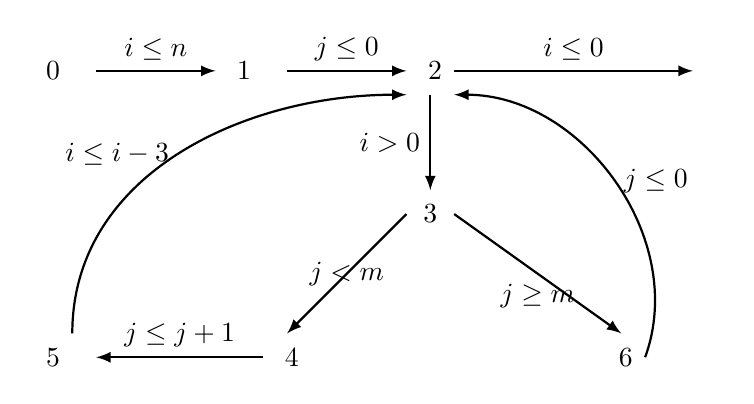
\begin{tikzpicture}[scale=\textwidth/20cm,samples=200]
  \draw[] (-8, 10) circle (0pt) node{{ $0$}};
  \draw[] (-4, 10) circle (0pt) node{{ $1$}};
  \draw[] (0, 10) circle (0pt) node{{ $2$}};
  \draw[] (0, 7) circle (0pt) node{{$3$}};
  \draw[] (-3, 4) circle (0pt) node{{ $4$}};
  \draw[] (-8, 4) circle (0pt) node{{ $5$}};
  \draw[] (4, 4) circle (0pt) node{{ $6$}};
  % Counter Variables
  \draw[] (6, 10) circle (0pt) node {\textbf{$\lex$}};
  % \draw[] (6, 4) circle (0pt) node {{ $ex$}};
  %
  % Control Flow Edges:
  \draw[ thick, -latex] (-7, 10)  -- node [above] {$i \leq n$}(-4.5, 10);
  \draw[ thick, -latex] (-3, 10)  -- node [above] {$j \leq 0$}(-0.5, 10);
  \draw[ thick, -latex] (0, 9.5)  -- node [left] {$i > 0$} (0, 7.5) ;
  \draw[ thick, -latex] (0.5, 7)  -- node [below] {$ j \geq m $}  (4, 4.5);
  \draw[ thick, -latex] (-7.5, 4.5)  to  [out=90,in=180]  node [left] {$i \leq i - 3$ }(-0.5, 9.5);
  \draw[ thick, -latex] (4.5, 4)  to  [out=70,in=0]   node [right] {$j \leq 0 $}(0.5, 9.5);
  \draw[ thick, -latex]  (-0.5, 7) -- node  {$j < m$}  (-3, 4.5) ;
  \draw[ thick, -latex]  (-3.5, 4) -- node [above] {$j \leq j + 1$}  (-7, 4) ;
  \draw[ thick, -latex] (0.5, 10)  -- node [above] {$i \leq 0$}  (5.5, 10);
  % \draw[ thick, -latex] (6, 6.5)  -- node [right] {$\top$} (6, 4.5) ;
  \end{tikzpicture}
  \caption{}
    \end{centering}
    \end{subfigure}
  \caption{
  (a) The Two Paths While Loop Example with Two Coutners
    (b) The Abstract Execution Control Flow Graph}
      \label{fig:twoCountersWhile}
  \end{figure}
  }
\end{example}

\begin{enumerate}
  \item  \textbf{The Abstract Execution Control Flow Graph} is generated in Figure~\ref{fig:twoCountersWhile}(b).

  \item \textbf{Program Rephrase and Refinement}. 
  \\
  The loop free transition paths are computed as follows,
  \[
    \begin{array}{ll}
\tpath_0 = (0 \to 1), (1 \to 2)
&
\tpath_2 = (2 \to 3), (3 \to 6), (6 \to 2)
\\
\tpath_1 = (2 \to 3), (3 \to 4), (4 \to 5), (5 \to 2)
&
\tpath_3 = (2 \to \lex)
\end{array}
\]
\textbf{Rephrased Program}:
\[
\tpath_0 ; LOOP1: \rprepeat(\rpchoose\{\tpath_1, \tpath_2 \}); \tpath_3
\]
\textbf{Refined Program}:
\[
  \tpath_0 ; LOOP1: \rpchoose\{\rprepeat_2(\rprepeat_1(\tpath_1); \tpath_2) , \rprepeat_1(\tpath_1) \}; \tpath_3
  \]
  \item \textbf{Outside-In Algorithm} : Compute Local Bound for Every program and sub programs.
  \[
    \begin{array}{l}
        LB(\tpath_0) = 1
        \\
        LB(\rprepeat_1(\tpath_1)) = m 
        \\
        LB(\rprepeat_2(\rprepeat_1(\tpath_1); \tpath_2)) = \lfloor\frac{n}{m}\rfloor
        \\
        LB(LOOP1: \rpchoose(\rprepeat_2(\cdots), \rprepeat_1(\tpath_1))) 
        = \max\{m, (m  + 1)\times \lfloor\frac{n}{m}\rfloor\}
\end{array}
\]
\item \textbf{Inside-Out Algorithm}
\begin{itemize}
  \item \textbf{Repeat Chain Set}
  \\
  $rp\mathcal{C}(LOOP1, \tpath_1) = \{\rprepeat_1(\tpath_1), \rprepeat_2(\rprepeat_1(\tpath_1); \tpath_2) \to \rprepeat_1(\tpath_1)\}$ \\
  $rp\mathcal{C}(LOOP1, \tpath_2) = \{\rprepeat_2(\cdots; \tpath_2) \to \rprepeat_1(\tpath_1)\}$ \\
  $rp\mathcal{C}(\_, \_) = \emptyset$ 
  % \\
  \item \textbf{{Local Repeat Chain Bound} }for Every Transition Path $\tpath$ on its Repeat Chain
  \\
  $rpLB(LOOP1, \tpath_1) = \max\{m, m \times \lfloor\frac{n}{m}\rfloor\}$ \\
  $rpLB(LOOP1, \tpath_2) = \lfloor\frac{n}{m}\rfloor$ 
  %
  \item \textbf{Loop Chain} Set
  \\
  $lp\mathcal{C}(\tpath_0) = \{\tpath_0\}$ \qquad
  $lp\mathcal{C}(\tpath_1) = \{LOOP1\to \tpath_1\}$ \\
  $lp\mathcal{C}(\tpath_3) = \{\tpath_3\}$ \qquad
  $lp\mathcal{C}(\tpath_2) = \{LOOP1\to \tpath_2\}$ 
  \item \textbf{Nested Loop Bound }for Every Transition Path $\tpath$ on its Loop Chain
  \\
  $rpLB(LOOP1, \tpath_1) = \max\{m, m \times \lfloor\frac{n}{m}\rfloor\}$ \quad
  $rpLB(LOOP1, \tpath_2) = \lfloor\frac{n}{m}\rfloor$  \\
  $rpLB(\bot, \tpath_0) = 1$ \quad
  $rpLB(\bot, \tpath_3) = 1$ 
  \item \textbf{Path Sensitive Reachability Bound For Every Transition Path $\tpath$ }
  \\
  $psRB(\tpath_1) = n$ \quad
  $psRB(\tpath_2) = \lfloor\frac{n}{m}\rfloor$ \quad
  $psRB(\tpath_0) = 1$ \quad
  $psRB(\tpath_3) = 1$ 
\end{itemize}
\item Step 7: Path Sensitive Reachability Bound Computation for Every Location
\\
$psRB(\{0, 1\}) = 1$ \qquad
$psRB(\{\lex\}) = 1$ \qquad
$psRB(\{6 \}) = \lfloor\frac{n}{m}\rfloor$ \\
$psRB(\{4, 5 \}) = \max\{m, m \times \lfloor\frac{n}{m}\rfloor\}$ \quad
$psRB(\{3, 2 \}) = \max\{m, m \times \lfloor\frac{n}{m}\rfloor\} + \lfloor\frac{n}{m}\rfloor + 1 $ \\
\end{enumerate}
\begin{example}[Nested Loop with Related Iterators]
  \label{ex:threeNestedWhile}
  %
  %
  { \small
\begin{figure}
\centering
\begin{subfigure}{.4\textwidth}
  \begin{centering}
  {\footnotesize
  $
  \begin{array}{l}
      \kw{relatedNestedWhile}(n, m, N) \triangleq \\
      \clabel{ \assign{i}{0} }^{0} ; \\
          \ewhile ~ \clabel{i < n}^{1} ~ \edo ~ \\
          \qquad \Big(
           \clabel{\assign{j}{m}}^{2} ;\\
           \qquad \ewhile ~ \clabel{j > 0}^{3} ~ \edo ~ \\
           \qquad \qquad \Big(
            \clabel{\assign{j}{j-1}}^{4};
            \clabel{\assign{w}{i}}^{5};\\
            \qquad \qquad \ewhile ~ \clabel{w < N}^{6} ~ \edo ~
            \Big(
              \clabel{\assign{w}{w + 1}}^{7}
                \Big); \\
                \qquad \qquad \clabel{\assign{i}{w}}^{8}
                \Big); \\
                \qquad \clabel{\assign{i}{i+1}}^{9}
            \Big)
      \end{array}
  $
  }
  \caption{}
  \end{centering}
  \end{subfigure}
\begin{subfigure}{.5\textwidth}
  \begin{centering}
%   \todo{abstract-cfg for two round}
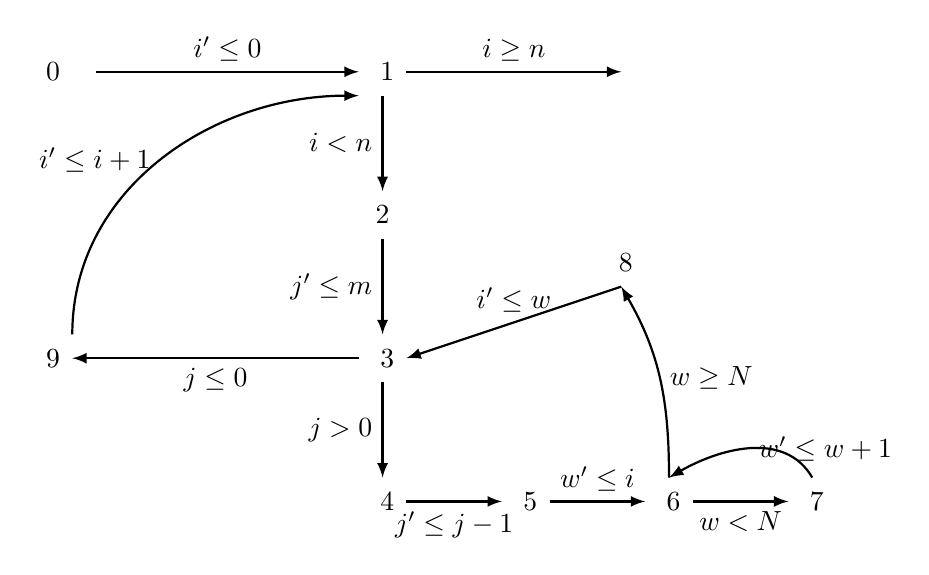
\begin{tikzpicture}[scale=\textwidth/20cm,samples=200]
\draw[] (-7, 10) circle (0pt) node{{ $0$}};
\draw[] (0, 10) circle (0pt) node{{ $1$}};
\draw[] (6, 10) circle (0pt) node {{$\lex$}};
\draw[] (0, 7) circle (0pt) node{{$2$}};
\draw[] (0, 4) circle (0pt) node{{ $3$}};
\draw[] (-7, 4) circle (0pt) node{{ $9$}};
\draw[] (0, 1) circle (0pt) node{{ $4$}};
\draw[] (3, 1) circle (0pt) node{{ $5$}};
\draw[] (6, 1) circle (0pt) node{{ $6$}};
\draw[] (9, 1) circle (0pt) node{{ $7$}};
\draw[] (5, 6) circle (0pt) node{{ $8$}};
% Counter Variables
%
% Control Flow Edges:
\draw[ thick, -latex] (-6, 10)  -- node [above] {$i' \leq 0$}(-0.5, 10);
\draw[ thick, -latex] (0, 9.5)  -- node [left] {$i < n$} (0, 7.5) ;
\draw[ thick, -latex] (0, 6.5)  -- node [left] {$j' \leq m$} (0, 4.5) ;
\draw[ thick, -latex] (0, 3.5)  -- node [left] {$j > 0$} (0, 1.5) ;
\draw[ thick, -latex] (-0.5, 4)  -- node [below] {$j \leq 0$} (-6.5, 4) ;
\draw[ thick, -latex] (-6.5, 4.5)  to  [out=90,in=180]  node [left] {$i' \leq i + 1$ }(-0.5, 9.5);
\draw[ thick, -latex] (0.5, 10)  -- node [above] {$i \geq n$}  (5, 10);
\draw[ thick, -latex] (0.5, 1)  -- node [below] {$j' \leq j - 1$}  (2.5, 1);
\draw[ thick, -latex] (3.5, 1)  -- node [above] {$w' \leq i$}  (5.5, 1);
\draw[ thick, -latex] (6.5, 1)  -- node [below] {$w < N$}  (8.5, 1);
\draw[ thick, -latex] (6, 1.5)  to [out=90,in=-60] node [right] {$w \geq N$}  (5, 5.5);
\draw[ thick, -latex] (9, 1.5)  to  [out=120,in=30] node [right] {$w' \leq w + 1$}  (6, 1.5);
\draw[ thick, -latex] (5, 5.5)  to  node [above] {$i' \leq w$ }(0.5, 4);
\end{tikzpicture}
\caption{}
  \end{centering}
  \end{subfigure}
\caption{
(a) The Example of Nested Loop with Related Iterators
  (b) The Abstract Execution Control Flow Graph}
    \label{fig:threeNestedWhile}
\end{figure}
}
\end{example}

\begin{enumerate}
  \item  \textbf{The Abstract Control Flow Graph}: Figure~\ref{fig:threeNestedWhile}(b).

  \item \textbf{Program Refinement}
  \\
  {Simple Transition Paths:}
  %  are computed as follows,
  \\
$
      \begin{array}{llll}
          \tpath_0 = (0 \to 1)
          &
          \tpath_1 = (1 \to 2 \to 3)
          &           
          \tpath_2 = (3 \to 4 \to 5 \to 6)
          &
          \tpath_3 = (6 \to 7 \to 6)
          \\
          \tpath_6 = (1 \to \lex)
          &
          \tpath_4 = (6 \to 8 \to 3)
          &
          \tpath_5 = (3 \to 9 \to 1)
      \end{array}
$
  \\
  Refined Program:
\\
$
  \rprog = \tpath_0 ; 
1: \rprepeat(\tpath_1; 3: \rprepeat(\tpath_2; 6: \rprepeat(\tpath_3); \tpath_4); \tpath_5); \tpath_6
$
\\
Let $\rprog_1 = \rprepeat(\tpath_1; 3: \rprepeat(\tpath_2; 6: \rprepeat(\tpath_3); \tpath_4); \tpath_5)$
\\
$\rprog_3 = \rprepeat(\tpath_2; 6: \rprepeat(\tpath_3); \tpath_4)$
\\
$\rprog_6 = \rprepeat(\tpath_3)$
  \item {Path Local Reachability-bound}:
\\
$\outinB(1: \rprog_1, \tpath_1) = n - N$ \quad
$\outinB(1: \rprog_1, \tpath_5) = n - N$ \quad
$\outinB(3: \rprog_3, \tpath_2) = m$ \\
$\outinB(3: \rprog_3, \tpath_4) = m$ \quad
$\outinB(6: \rprog_6, \tpath_3) = N$ \quad
%
\\
Loop Bounds:
\\
$BD(\tpath_0) = 1$
\quad
$BD(\tpath_6) = 1$
\quad
$BD( \rprepeat(\tpath_3)) = N $
\quad
$BD(\rprog_3) = m $
\quad
$BD(\rprog_1) = n - N $
%
\item Loop Reachability-bound:
\\
\highlight{
$\lpchB(1: \rprog_1, \tpath_1) = n - N$ \quad
$\lpchB(1: \rprog_1, \tpath_5) = n - N$ \quad
$\lpchB(1: \rprog_1, \tpath_2) = n$ \\ 
$\lpchB(1: \rprog_1, \tpath_4) = n$ \quad
$\lpchB(1: \rprog_1, \tpath_3) = 1$ \quad
$\lpchB(3: \rprog_3, \tpath_4) = m$ \\
$\lpchB(3: \rprog_3, \tpath_2) = m$ \quad
$\lpchB(3: \rprog_3, \tpath_3) = 1$ \quad 
$\lpchB(6: \rprog_6, \tpath_3) = N$
}
%
%
\item Path Global Reachability-bound:
\\
$\inoutB(\rprog, \tpath_1) = n - N$ \quad
$\inoutB(\rprog, \tpath_2) = n \times m$ \quad
$\inoutB(\rprog, \tpath_0) = 1$ 
\quad
$\inoutB(\rprog, \tpath_5) = n - N$ \quad
$\inoutB(\rprog, \tpath_4) = n \times m$ \quad
$\inoutB(\rprog, \tpath_6) = 1$ 
\quad
$\inoutB(\rprog, \tpath_3) = N$
%
\item The Reachability-bound:
\\
$\psRB(0) = \psRB(\lex) = 1$ \quad
$\psRB(1) = n - N + 1$ \quad
$\psRB(2) = \psRB(9) = n - N$ \quad
$\psRB(7) = N$
\\
$\psRB(3) = n - N + n \times m$ \quad
$\psRB(4) = \psRB(5) = \psRB(8) = n \times m$ \quad
$\psRB(6) = N + n \times m$ 
\end{enumerate}
\begin{example}[A Simplified Nested Loop with Related Iterator Example]
  \label{ex:relatedNestedWhileSim}
  %
  %
  { \small
\begin{figure}
\centering
\begin{subfigure}{.4\textwidth}
  \begin{centering}
  {\footnotesize
  $
  \begin{array}{l}
      \kw{relatedNestedWhileSim}(n, m, N) \triangleq \\
      \clabel{ \assign{i}{0} }^{0} ; \\
          \ewhile ~ \clabel{i < n}^{1} ~ \edo ~ \\
          \qquad \Big(
            \clabel{\assign{w}{i}}^{2};\\
            \qquad \ewhile ~ \clabel{w < N}^{3} ~ \edo ~
            \Big(
              \clabel{\assign{w}{w + 1}}^{4}
                \Big); \\
                \qquad \clabel{\assign{i}{w}}^{5};
                \clabel{\assign{i}{i+1}}^{6}
            \Big)
      \end{array}
  $
  }
  \caption{}
  \end{centering}
  \end{subfigure}
\begin{subfigure}{.5\textwidth}
  \begin{centering}
%   \todo{abstract-cfg for two round}
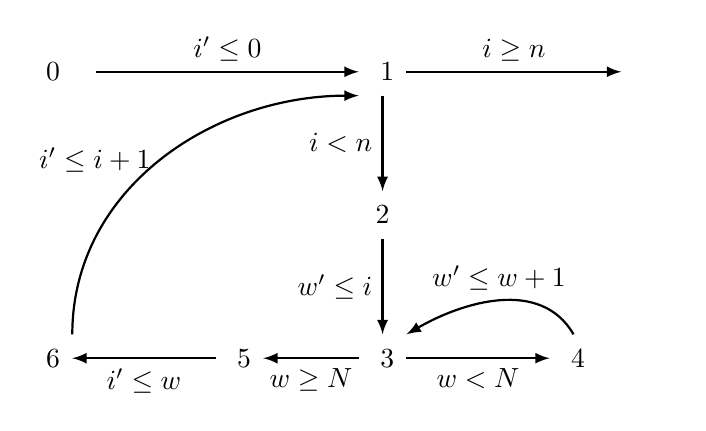
\begin{tikzpicture}[scale=\textwidth/20cm,samples=200]
\draw[] (-7, 10) circle (0pt) node{{ $0$}};
\draw[] (0, 10) circle (0pt) node{{ $1$}};
\draw[] (6, 10) circle (0pt) node {{$\lex$}};
\draw[] (0, 7) circle (0pt) node{{$2$}};
\draw[] (0, 4) circle (0pt) node{{ $3$}};
\draw[] (-7, 4) circle (0pt) node{{ $6$}};
\draw[] (-3, 4) circle (0pt) node{{ $5$}};
\draw[] (4, 4) circle (0pt) node{{ $4$}};
% Counter Variables
%
% Control Flow Edges:
\draw[ thick, -latex] (-6, 10)  -- node [above] {$i' \leq 0$}(-0.5, 10);
\draw[ thick, -latex] (0, 9.5)  -- node [left] {$i < n$} (0, 7.5) ;
\draw[ thick, -latex] (0, 6.5)  -- node [left] {$w' \leq i$} (0, 4.5) ;
\draw[ thick, -latex] (-0.5, 4)  -- node [below] {$w \geq N$} (-2.5, 4) ;
\draw[ thick, -latex] (-3.5, 4)  -- node [below] {$i' \leq w$} (-6.5, 4) ;
\draw[ thick, -latex] (-6.5, 4.5)  to  [out=90,in=180]  node [left] {$i' \leq i + 1$ }(-0.5, 9.5);
\draw[ thick, -latex] (0.5, 10)  -- node [above] {$i \geq n$}  (5, 10);
\draw[ thick, -latex] (4, 4.5)  to  [out=120,in=30] node [above] {$w' \leq w + 1$}  (0.5, 4.5);
\draw[ thick, -latex] (0.5, 4)  -- node [below] {$w < N$}  (3.5, 4);
\end{tikzpicture}
\caption{}
  \end{centering}
  \end{subfigure}
\caption{
(a) The Simplified Example of Nested Loop with Related Iterator
  (b) The Abstract Execution Control Flow Graph}
    \label{fig:relatedNestedWhileSim}
\end{figure}
}
\end{example}

\begin{enumerate}
  \item  \textbf{The Constraint Program (Abstract Control Flow Graph)} is generated in Figure~\ref{fig:threeNestedWhile}(b).

  \item \textbf{Program Refinement}
  \\
  The loop free simple transition paths are computed as follows,
  \[
      % \begin{array}{lllll}
          \tpath_0 = (0 \to 1)
          \quad
          \tpath_1 = (1 \to 2 \to 3)
          \quad           
          \tpath_2 = (3 \to 4 \to 3)
          \quad
          \tpath_3 = (3 \to 5 \to 6 \to 1)
          \quad
          \tpath_4 = (1 \to \lex)
      % \end{array}
      \]
  \textbf{Refined Program}:
  \[
  \rprog = \tpath_0 ; 1: \rprepeat(\tpath_1; 3: \rprepeat(\tpath_2); \tpath_3); \tpath_4
  \]
  \item \textbf{Outside-In Algorithm}: The \emph{OutIn} bound for the $\rprog$ and every nested repeat patterns.
  \\
$\outinB(\tpath_0) = 1$
\quad
$\outinB(3: \rprepeat(\tpath_2)) = N $
\\
$\outinB(1: \rprepeat(\tpath_1; 3: \rprepeat(\tpath_2); \tpath_3)) = n - N $
\item \textbf{Inside-Out Algorithm}
\begin{itemize}
  \item \textbf{Repeat Chain Set}
  \\
  $\rpchset(1, \tpath_1) = \{\rprepeat(\tpath_1; 3: \rprepeat(\tpath_2); \tpath_3)\}$
  \\
  $\rpchset(1, \tpath_3) = \{\rprepeat(\tpath_1; 3: \rprepeat(\tpath_2); \tpath_3)\}$
  \\
  $\rpchset(3, \tpath_2) = \{\rprepeat(\tpath_2)\}$ \quad
  $\rpchset(_, \_) = \emptyset$ 
  % \\
  \item \textbf{Repeat Chain Bound} for every simple transition path $\tpath$ through its \emph{Repeat Chain}s
  \\
  $\rpchB(1, \tpath_1) = n - N$ \quad
  $\rpchB(1, \tpath_3) = n - N$ \quad
  $\rpchB(3, \tpath_2) = N$ \quad
  $\rpchB(_, \_) = \bot $ 
  %
  \item \textbf{Loop Chain}
  \\
  $\lpch(\tpath_1) = 1\to \tpath_1$ \quad
  \highlight{$\lpch(\tpath_2) = 1 \to 3 \to \tpath_2$} \quad
  $\lpch(\tpath_3) = 1 \to \tpath_3$ \\
  $\lpch(\tpath_0) = \tpath_0$ \quad
  $\lpch(\tpath_4) = \tpath_4$
  \item \textbf{{Relative Loop Bound}} for every simple transition path $\tpath$ through its \emph{Loop Chain}
  \\
  $\rpchB(1, \tpath_1) = n - N$ \quad
  $\rpchB(1, \tpath_3) = n - N$ \quad
  \highlight{$\rpchB(1, \tpath_2) = 1$} \quad
  $\rpchB(3, \tpath_2) = N$ \quad
  $\rpchB(_, \_) = 1 $ 
  \item \textbf{Path-Sensitive Reachability-Bound} for every simple transition path $\tpath$
  \\
  $\inoutB(\tpath_1) = n - N$ \quad
  $\inoutB(\tpath_2) = N$ \quad
  $\inoutB(\tpath_0) = 1$ 
  \\
  \highlight{ $\inoutB(\tpath_3) = n - N$} \quad
  $\inoutB(\tpath_4) = 1$ 
  \end{itemize}
\item \textbf{Path Sensitive Reachability-Bound} on every program control location
\\
$\psRB(\{0, \lex\}) = 1$ \quad
$\psRB(\{1\}) = n - N + 1$ \quad
$\psRB(\{2, 5, 6\}) = n - N$ \\
\highlight{$\psRB(\{3\}) = N + 1 + n - N = n + 1$} \quad
$\psRB(\{4\}) = N$
\end{enumerate}
\begin{example}[Nested Loop with Variable Reset Chain]
  \label{ex:nestedWhileResetChain}
  %
  %
  { \small
\begin{figure}
\centering
\begin{subfigure}{.4\textwidth}
  \begin{centering}
  {\small
  $
  \begin{array}{l}
      \kw{nestedWhileResetChain}(n) \triangleq \\
      \clabel{ \assign{i}{n} }^{0} ; \\
      \clabel{ \assign{r}{n} }^{1} ; \\
          \ewhile ~ \clabel{i > 0}^{2} ~ \edo ~ \\
          \qquad \Big( \clabel{\assign{r}{r + 1}}^{3};\\
            \qquad  \clabel{\assign{k}{r}}^{4};\\
            \qquad \ewhile ~ \clabel{k > 0}^{5} ~ \edo ~
            \Big( \clabel{\assign{k}{k - 1}}^{6}   \Big); \\
                \qquad \clabel{\assign{r}{k}}^{7};
                \clabel{\assign{i}{i-1}}^{8}
            \Big)
      \end{array}
  $
  }
  \caption{}
  \end{centering}
  \end{subfigure}
\begin{subfigure}{.5\textwidth}
  \begin{centering}
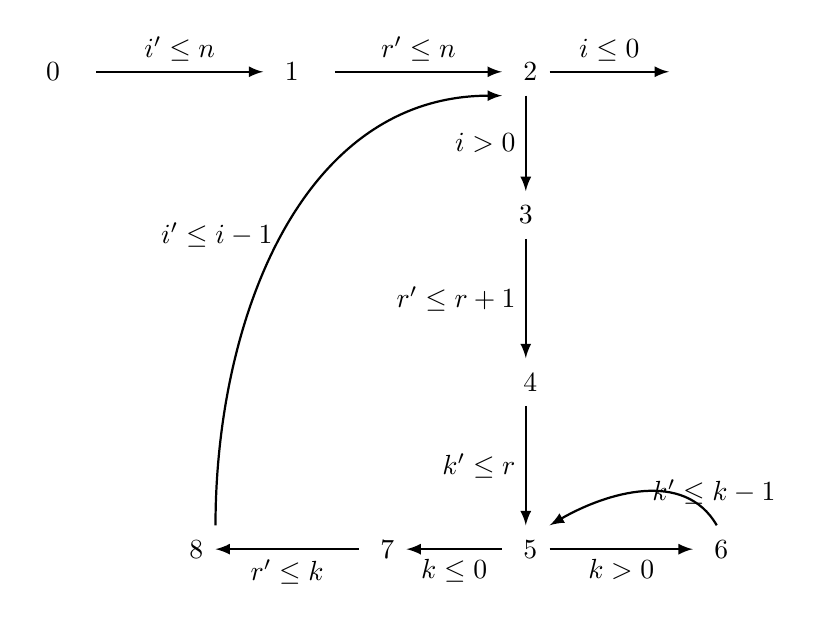
\begin{tikzpicture}[scale=\textwidth/20cm,samples=200]
\draw[] (-10, 10) circle (0pt) node{{ $0$}};
\draw[] (-5, 10) circle (0pt) node{{ $1$}};
\draw[] (0, 10) circle (0pt) node{{ $2$}};
\draw[] (4, 10) circle (0pt) node {{$\lex$}};
%
\draw[] (0, 7) circle (0pt) node{{$3$}};
\draw[] (0, 3.5) circle (0pt) node{{ $4$}};
\draw[] (0, 0) circle (0pt) node{{ $5$}};
\draw[] (4, 0) circle (0pt) node{{ $6$}};
%
\draw[] (-3, 0) circle (0pt) node{{ $7$}};
\draw[] (-7, 0) circle (0pt) node{{ $8$}};
% Counter Variables
%
% Control Flow Edges:
\draw[ thick, -latex] (-9, 10)  -- node [above] {$i' \leq n$}(-5.5, 10);
\draw[ thick, -latex] (-4, 10)  -- node [above] {$r' \leq n$}(-0.5, 10);
\draw[ thick, -latex] (0.5, 10)  -- node [above] {$i \leq 0 $}  (3, 10);
\draw[ thick, -latex] (0, 9.5)  -- node [left] {$i > 0$} (0, 7.5) ;
\draw[ thick, -latex] (0, 6.5)  -- node [left] {$r' \leq r + 1$} (0, 4) ;
\draw[ thick, -latex] (0, 3)  -- node [left] {$k' \leq r$} (0, 0.5) ;
% While Guard True, Loop Body
\draw[ thick, -latex] (0.5, 0)  -- node [below] {$k > 0$}  (3.5, 0);
\draw[ thick, -latex] (4, 0.5)  to  [out=120,in=30] node [right] {$k' \leq k - 1$}  (0.5, 0.5);
% While Guard IS FALSE, RETURN BACK TO THE PREVIOUS CONTROL POINT
\draw[ thick, -latex] (-0.5, 0)  -- node [below] {$k \leq 0$} (-2.5, 0) ;
\draw[ thick, -latex] (-3.5, 0)  -- node [below] {$r' \leq k$} (-6.5, 0) ;
\draw[ thick, -latex] (-6.5, 0.5)  to  [out=90,in=180]  node [left] {$i' \leq i - 1$ }(-0.5, 9.5);
\end{tikzpicture}
\caption{}
  \end{centering}
  \end{subfigure}
\caption{
(a) The Simplified Example of Nested Loop with Related Iterator
  (b) The Abstract Execution Control Flow Graph}
    \label{fig:nestedWhileResetChain}
\end{figure}
}
\end{example}

\begin{enumerate}
  \item  \textbf{Abstract Control Flow Graph} is generated in Figure~\ref{fig:nestedWhileResetChain}(b).

  \item \textbf{Program Refinement}
  \\
  The loop free simple transition paths:
  \[
      % \begin{array}{lllll}
          \tpath_0 = (0 \to 1 \to 2)
          \quad
          \tpath_1 = (2 \to 3 \to 4 \to 5)
          \quad           
          \tpath_2 = (5 \to 6 \to 5)
          \quad
          \tpath_3 = (5 \to 7 \to 8 \to 2)
          \quad
          \tpath_4 = (2 \to \lex)
      % \end{array}
      \]
  \textbf{Refined Program}:
  \[
  \rprog = \tpath_0 ; 2: \rprepeat(\tpath_1; 5: \rprepeat(\tpath_2); \tpath_3); \tpath_4
  \]
Let $\rprog_2 = \rprepeat(\tpath_1; 5: \rprepeat(\tpath_2); \tpath_3)$
\item {Path Local Reachability Bound}:
\\
$\outinB(\rprog, \tpath_0) = 1$ \quad
$\outinB(\rprog, \tpath_4) = 1$ \\
$\outinB(2: \rprog_2, \tpath_1) = n$ \quad
$\outinB(2: \rprog_2, \tpath_3) = n$ \\
$\outinB(5: \rprepeat(\tpath_2), \tpath_2) = n + 1$
%
\\
Loop Bounds:
\\
$BD(\tpath_0) = 1$
\quad
$BD(\tpath_4) = 1$
\quad
$BD(\rprepeat(\tpath_2)) = n + 1 $
\\
$BD(\rprepeat(\tpath_1; 5: \rprepeat(\tpath_2); \tpath_3)) = n $
%
\item Loop Reachability Bound:
\\
\highlight{
$\lpchB(2: \rprog_2, \tpath_1) = n$ \quad
$\lpchB(2: \rprog_2, \tpath_3) = n$ \quad 
$\lpchB(2: \rprog_2, \tpath_2) = \frac{(n + 1) - 0}{n}$ 
\\
$\lpchB(5: \rprepeat(\tpath_2), \tpath_2) = n + 1$ \\
$\lpchB(2: \rprog_2, \tpath_4) = 0$ \quad
$\lpchB(2: \rprog_2, \tpath_0) = 0$ \quad
$\lpchB(2: \rprog_2, \tpath_0) = 0$ \quad
}
%
%
\item Path Global Reachability Bound:
\\
$\inoutB(\rprog, \tpath_0) = 1$ \quad
$\inoutB(\rprog, \tpath_1) = n$ \quad
$\inoutB(\rprog, \tpath_2) = \frac{(n + 1)^2}{n}$ \\
$\inoutB(\rprog, \tpath_3) = n$ \quad
$\inoutB(\rprog, \tpath_4) = 1$
%
\item The Reachability Bound:
\\
$\psRB(0) = \psRB(1) = \psRB(\lex) = 1$ \quad
$\psRB(2) = n + 1$ \\
$\psRB(3) = \psRB(4) =\psRB(7) = \psRB(8) = n$ \quad \\
$\psRB(6) = \frac{(n + 1)^2}{n} $ \quad
\highlight{$\psRB(\{5\}) = n + \frac{(n + 1)^2}{n}$}
\end{enumerate}
% \begin{example}
    [While Odds Algorithm]
    \label{ex:whileOdd}
    \[
      %
      \begin{array}{l}
          \kw{whileOdd}(k) \triangleq \\
          \clabel{ \assign{i}{k} }^{0} ; \\
              \ewhile ~ \clabel{i > 0}^{1} ~ \edo ~ \\
              \qquad \Big(
                \eif(\clabel{i \% 2 == 0 }^{2}, \\
                \qquad \qquad \clabel{\assign{i}{i - 1}}^{3},\\
                \qquad \qquad \clabel{\assign{i}{i - 3}}^{4});
                \Big)
          \end{array}
      \]
    % \end{example}
    { \small
    \begin{figure}
    \centering
    %
    \begin{subfigure}{.4\textwidth}
        \begin{centering}
        \begin{tikzpicture}[scale=\textwidth/15cm,samples=200]
    % Variables Initialization
    \draw[] (5, 1) circle (0pt) node{{ $x^1: {}^1_{1}$}};
    % Variables Inside the Loop
     \draw[] (0, 7) circle (0pt) node{\highlight{ $y^5: {}^{\frac{k}{2}}_{1}$}};
     \draw[] (0, 4) circle (0pt) node{\highlight{ \boldsymbol{$p^6: {}^{\frac{k}{2}}_{1}$}}};
     \draw[] (0, 1) circle (0pt) node{{ $\mathbf{x^7: {}^{k}_{1}}$}};
     % Counter Variables
     \draw[] (5, 7) circle (0pt) node {{$j^0: {}^{1}_{0}$}};
     \draw[] (5, 4) circle (0pt) node {{ $j^3: {}^{k}_{0}$}};
     %
    % Value Dependency Edges:
             % Value Dependency Edges:
             \draw[ thick, -latex,]  (0, 3.5) -- 
             node [] {\highlight{$k $}}(0, 1.5) ;
             \draw[ thick, -Straight Barb] (6.5, 4.5) arc (150:-150:1);
             \draw[](7, 4) node [] {\highlight{$k  $}};
             \draw[ thick, -latex] (5, 4.5)  -- 
             node [right] {\highlight{$k$}}(5, 6.5) ;
             % Value Dependency Edges on Initial Values:
             \draw[ thick, -latex,] (1.5, 1)  -- 
             node [above] {\highlight{$k$}}(4, 1) ;
             %
            \draw[ ultra thick, -latex, densely dotted,] (-0.6, 1.5)  to  [out=-220,in=220]  
            node [left] {\highlight{$k $}}(-0.5, 6.5);
            \draw[ ultra thick, -latex, densely dotted,]  (0.5, 6.5) to  [out=-30,in=30] 
            node [above] {\highlight{$k $}}(0.6, 1.6) ;
             % Control Dependency
            \draw[ thick,-latex] (1.5, 7)  -- 
            node [above] {\highlight{$k$}}(4, 6) ;
            \draw[ thick,-latex] (1.5, 4)  -- 
            node [above] {\highlight{$k$}}(4, 6) ;
             \draw[ thick,-latex] (1.5, 1)  -- 
             node [below] {\highlight{$k $}}(4, 6) ;
    
    \end{tikzpicture}
    \caption{}
    \end{centering}
    \end{subfigure}
    %
            \begin{subfigure}{.5\textwidth}
                \begin{centering}
                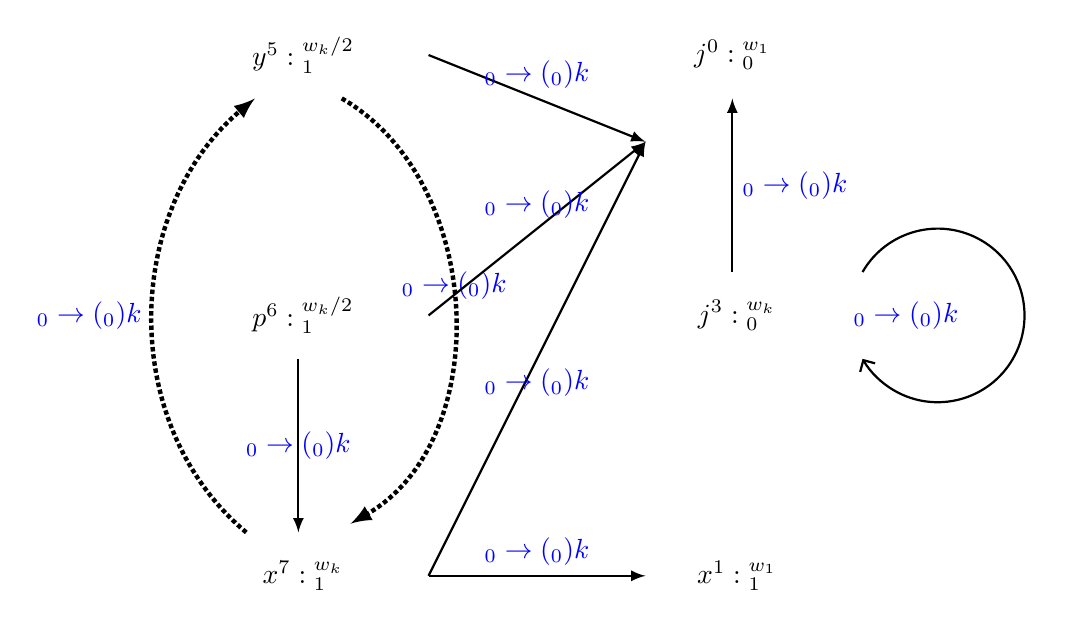
\begin{tikzpicture}[scale=\textwidth/11cm,samples=200]
            % Variables Initialization
             \draw[] (5, 1) circle (0pt) node{{ $x^1: {}^{w_1}_{1}$}};
            % Variables Inside the Loop
             \draw[] (0, 7) circle (0pt) node{{ $y^5: {}^{w_k/2}_{1}$}};
             \draw[] (0, 4) circle (0pt) node{{ $p^6: {}^{w_k/2}_{1}$}};
             \draw[] (0, 1) circle (0pt) node{{ $x^7: {}^{w_k}_{1}$}};
             % Counter Variables
             \draw[] (5, 7) circle (0pt) node {{$j^0: {}^{w_1}_{0}$}};
             \draw[] (5, 4) circle (0pt) node {{ $j^3: {}^{w_k}_{0}$}};
             %
             % Value Dependency Edges:
             \draw[ thick, -latex,]  (0, 3.5) -- 
             node [] {\highlight{$\trace_0 \to \env(\trace_0) k $}}(0, 1.5) ;
             \draw[ thick, -Straight Barb] (6.5, 4.5) arc (150:-150:1);
             \draw[](7, 4) node [] {\highlight{$\trace_0 \to \env(\trace_0) k  $}};
             \draw[ thick, -latex] (5, 4.5)  -- 
             node [right] {\highlight{$\trace_0 \to \env(\trace_0) k $}}(5, 6.5) ;
             % Value Dependency Edges on Initial Values:
             \draw[ thick, -latex,] (1.5, 1)  -- 
             node [above] {\highlight{$\trace_0 \to \env(\trace_0) k $}}(4, 1) ;
             %
            \draw[ ultra thick, -latex, densely dotted,] (-0.6, 1.5)  to  [out=-220,in=220]  
            node [left] {\highlight{$\trace_0 \to \env(\trace_0) k $}}(-0.5, 6.5);
            \draw[ ultra thick, -latex, densely dotted,]  (0.5, 6.5) to  [out=-30,in=30] 
            node [above] {\highlight{$\trace_0 \to \env(\trace_0) k $}}(0.6, 1.6) ;
             % Control Dependency
            \draw[ thick,-latex] (1.5, 7)  -- 
            node [above] {\highlight{$\trace_0 \to \env(\trace_0) k $}}(4, 6) ;
            \draw[ thick,-latex] (1.5, 4)  -- 
            node [above] {\highlight{$\trace_0 \to \env(\trace_0) k $}}(4, 6) ;
             \draw[ thick,-latex] (1.5, 1)  -- 
             node [below] {\highlight{$\trace_0 \to \env(\trace_0) k $}}(4, 6) ;
             \end{tikzpicture}
             \caption{}
                \end{centering}
                \end{subfigure}
    \caption{
    (a) The multiple rounds odd example 
    (b) The program-based dependency graph from $\THESYSTEM$
    (c) The execution-based dependency graph.}
        \label{fig:overappr_example}
    \end{figure}
    }
    %
    \end{example}    
    \begin{enumerate}
      \item Step 1: Abstract Transition Graph:
    
    \item Step 2: Path Insensitive Transition Bound Computation
    
    \item Step 3: Program Rephrase through Path Collection on Abstract CFG
    \\
    $\tpath_0 = (0, 1)$
    \\
    $\tpath_1 = (1 \to 2), (2 \to 3), (3 \to 1)$
    \\
    $\tpath_2 = (1 \to 2), (2 \to 4), (4 \to 1)$
    \\
    $\tpath_3 = (1 \to \lex)$
    \\
    Rephrased Program
    \[
    \tpath_0 ; LOOP1: \rprepeat(\rpchoose\{\tpath_1, \tpath_2 \}); \tpath_3
    \]
    \item Step 4: While Loop Refinement:
    \[
      \tpath_0 ; LOOP1: \rpchoose\{\rprepeat_3(\rprepeat_1(\tpath_1); \tpath_2) , \rprepeat_4(\rprepeat_2(\tpath_2); \tpath_1) \}; \tpath_3
      \]
    \item Step 5: Outside-In Algorithm
    \\
    $LB(\tpath_0) = 1$
    \\
    $LB(\tpath_3) = 1$
    \\
    $LB(\rprepeat_1(\tpath_1)) = 1 $
    \\
    $LB(\rprepeat_3(\rprepeat_1(\tpath_1); \tpath_2)) = \frac{n}{4} $
    \\
    $LB(\rprepeat_2(\tpath_2)) = 1 $
    \\
    $LB(\rprepeat_4(\rprepeat_2(\tpath_2); \tpath_1)) = \frac{n}{4} $
    % \\
    % $LB(LOOP1: \rpchoose(\rprepeat_2(\cdots), \rprepeat_1(\tpath_1))) 
    % = \max\{m, \frac{n}{m}\} $
    % \\
    \item Step 6: Inside-Out Algorithm
    \begin{itemize}
      \item \textbf{Repeat Chain Set}
      \\
      $rp\mathcal{C}(LOOP1, \tpath_1) = \{\rprepeat_4(\cdots, \tpath_1), \rprepeat_3(\rprepeat_1(\tpath_1); \tpath_2) \to \rprepeat_1(\tpath_1)\}$ \\
      $rp\mathcal{C}(LOOP1, \tpath_2) = \{\rprepeat_3(\cdots, \tpath_2), \rprepeat_4(\rprepeat_2(\tpath_2); \tpath_1) \to \rprepeat_2(\tpath_2)\}$ \\
      $rp\mathcal{C}(\_, \_) = \emptyset$ 
      % \\
      \item \textbf{{Local Repeat Chain Bound} for Every Transition Path $\tpath$ on its Repeat Chain}
      $rpLB(LOOP1, \tpath_1) = \frac{n}{4}$ \\
      $rpLB(LOOP1, \tpath_2) = \frac{n}{4}$ 
      %
      \item \textbf{Loop Chain}
      \\
      $lp\mathcal{C}(\tpath_1) = \{LOOP1\to \tpath_1\}$ \\
      $lp\mathcal{C}(\tpath_2) = \{LOOP1\to \tpath_2\}$ \\
      $lp\mathcal{C}(\tpath_0) = \{\tpath_0\}$ \\
      $lp\mathcal{C}(\tpath_3) = \{\tpath_3\}$ 
      \item \textbf{Nested Loop Bound for Every Transition Path $\tpath$ on its Loop Chain}
      \\
      $rpLB(LOOP1, \tpath_1) = \frac{n}{4}$ \\
      $rpLB(LOOP1, \tpath_2) = \frac{n}{4}$  \\
      $rpLB(\bot, \tpath_0) = 1$ \\
      $rpLB(\bot, \tpath_3) = 1$ 
      \item \textbf{Path Sensitive Reachability Bound For Every Transition Path $\tpath$ }
      \\
      $psRB(\tpath_1) = \frac{n}{4}$ \\
      $psRB(\tpath_2) = \frac{n}{4}$ \\
      $psRB(\tpath_0) = 1$ \\
      $psRB(\tpath_3) = 1$ 
    \end{itemize}
    \item Step 7: Path Sensitive Reachability Bound Computation for Every Location
    \\
    $psRB(\{0, 1\}) = 1$ \\
    $psRB(\{2, 3, 1 \}) = \frac{n}{4}$ \\
    $psRB(\{2, 4, 1\}) = \frac{n}{4}$ \\
    $psRB(\{\lex\}) = 1$ 
    \end{enumerate}


% \begin{example}
    [While Single Algorithm]
    \label{ex:whileSigle}
    \[
      %
      \begin{array}{l}
          \kw{whileSingle}(k) \triangleq \\
          \clabel{ \assign{i}{k} }^{0} ; \\
              \ewhile ~ \clabel{i > 0}^{1} ~ \edo ~ \\
              \qquad \Big(
                \eif(\clabel{i = 2 }^{2}, \\
                \qquad \qquad \clabel{\assign{i}{i - 2}}^{3},\\
                \qquad \qquad \clabel{\assign{i}{i - 1}}^{4});
                \Big)
          \end{array}
      \]
    % \end{example}

    \begin{figure}
      \centering
     \begin{subfigure}{.6\textwidth}
         \begin{centering}
         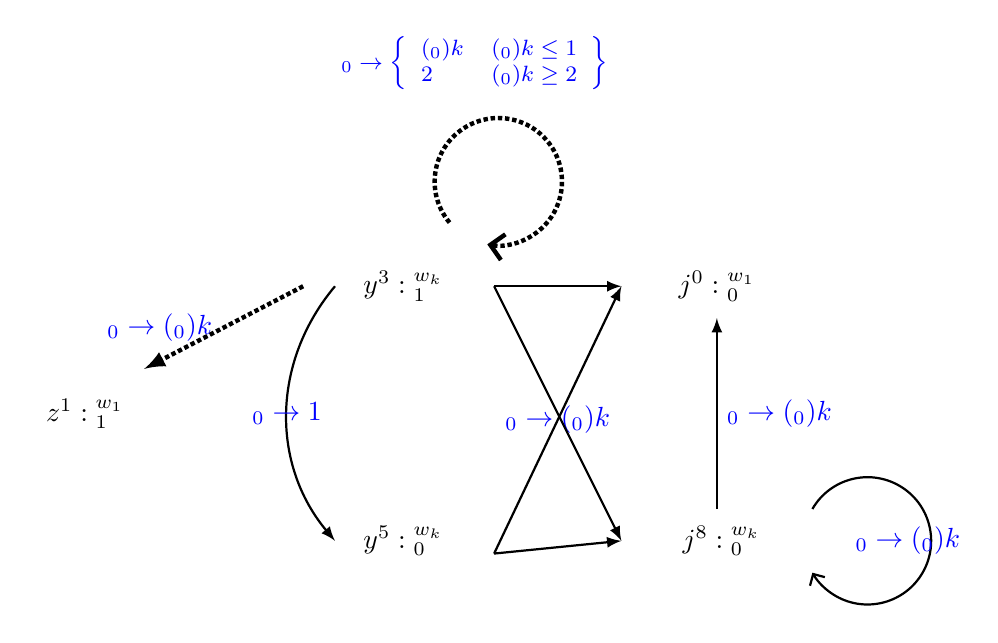
\begin{tikzpicture}[scale=\textwidth/15cm,samples=150]
     % Variables Initialization
     % \draw[] (-5, 1) circle (0pt) node{{ $z^1: {}^{w_1}_{1}$}};
     % \draw[] (-5, 7) circle (0pt) node{{$p^2: {}^{w_1}_{0}$}};
     \draw[] (-5, 4) circle (0pt) node{{ $z^1: {}^{w_1}_{1}$}};
     % Variables Inside the Loop
      \draw[] (0, 6) circle (0pt) node{{ $y^3: {}^{w_k}_{1}$}};
      \draw[] (0, 2) circle (0pt) node{{ $y^{5}: {}^{w_k}_{0}$}};
      % Counter Variables
      \draw[] (5, 6) circle (0pt) node {{$j^0: {}^{w_1}_{0}$}};
      \draw[] (5, 2) circle (0pt) node {{ $j^8: {}^{w_k}_{0}$}};
      %
      % Value Dependency Edges:
      \draw[ ultra thick, -Straight Barb, densely dotted,] (0.8, 7) arc (220:-100:1);
      % The Weight for this edge
      \draw[](1.2, 9.5) node 
      {\highlight{\footnotesize
             $\trace_0 \to 
             \left\{\begin{array}{ll}
                \env(\trace_0) k & \env(\trace_0) k  \leq 1 \\
            2 & \env(\trace_0) k \geq 2
             \end{array}\right\}
             $}};
      \draw[ thick, -latex] (-1, 6)  to  [out=-130,in=130]  
     % The Weight for this edge
     node [] {\highlight{$\trace_0 \to 1 $}} (-1, 2);
      % Value Dependency Edges on Initial Values:
      \draw[ ultra thick, -latex, densely dotted,] (-1.5, 6)  -- 
     % The Weight for this edge
     node [left] {\highlight{$\trace_0 \to \env(\trace_0) k $}} (-4, 4.7) ;
      %
      % Value Dependency For Control Variables:
      \draw[ thick, -Straight Barb] (6.5, 2.5) arc  (150:-150:1);
     % The Weight for this edge
     \draw[](8, 2) node [] {\highlight{$\trace_0 \to \env(\trace_0) k  $}};
      % Control Dependency
      \draw[ thick, -latex] (5, 2.5)  -- 
     % The Weight for this edge
     node [right] {\highlight{$\trace_0 \to \env(\trace_0) k $}} (5, 5.5);
      \draw[ thick,-latex] (1.5, 6)  -- (3.5, 6) ;
      \draw[ thick,-latex] (1.5, 1.8)  -- 
     % The Weight for this edge
     node [] {\highlight{$\trace_0 \to \env(\trace_0) k $}} (3.5, 6) ;
      \draw[ thick,-latex] (1.5, 6)  -- (3.5, 2) ;
      \draw[ thick,-latex] (1.5, 1.8)  -- (3.5, 2) ; 
     \end{tikzpicture}
      \caption{}
         \end{centering}
         \end{subfigure}
     % \end{wrapfigure}
     % \end{equation*}
    %  \vspace{-0.4cm}
      \caption{(a) The multi rounds single example
      (b) The execution-based dependency graph.}
     \label{fig:multipleRoundsSingle}
     \end{figure}
     \end{example}

    \begin{enumerate}
      \item Step 1: Abstract Transition Graph:
    
    \item Step 2: Path Insensitive Transition Bound Computation
    
    \item Step 3: Program Rephrase through Path Collection on Abstract CFG
    \\
    $\tpath_0 = (0 \to 1)$
    \\
    $\tpath_1 = (1 \to 2), (2 \to 3), (3 \to 1)$
    \\
    $\tpath_2 = (1 \to 2), (2 \to 4), (4 \to 1)$
    \\
    $\tpath_3 = (1 \to \lex)$
    \\
    Rephrased Program
    \[
    \tpath_0 ; LOOP1: \rprepeat(\rpchoose\{\tpath_1, \tpath_2 \}); \tpath_3
    \]
    \item Step 4: While Loop Refinement:
    \[
      \tpath_0 ; 
      LOOP1: \rpchoose\{\rprepeat_1(\tpath_1), \rprepeat_2(\tpath_2),
      \rprepeat_3(\rprepeat_2(\tpath_2); \tpath_1)\}; \tpath_3
      \]
    \item Step 5: Outside-In Algorithm
    \\
    $LB(\tpath_0) = 1$
    \\
    $LB(\tpath_3) = 1$
    \\
    $LB(\rprepeat_1(\tpath_1)) = 1 $
    \\
    $LB(\rprepeat_2(\tpath_2)) = 
    \left\{
      \begin{array}{ll}
      \max\{0, n\} & \env(\trace_0) n < 2 \\
      n - 2 & \env(\trace_0)  n \geq 2
      \end{array} 
    \right.$
    \\
    $LB(\rprepeat_3(\rprepeat_1(\tpath_1); \tpath_2)) = 
    \left\{
      \begin{array}{ll}
      0 & \env(\trace_0) n \leq 2 \\
      1 & \env(\trace_0)  n > 2
      \end{array} 
    \right.$
    \\
    % \\
    % $LB(LOOP1: \rpchoose(\rprepeat_2(\cdots), \rprepeat_1(\tpath_1))) 
    % = \max\{m, \frac{n}{m}\} $
    % \\
    \item Step 6: Inside-Out Algorithm
    \begin{itemize}
      \item \textbf{Repeat Chain Set}
      \\
      $rp\mathcal{C}(LOOP1, \tpath_1) = \{\rprepeat_3(\cdots, \tpath_1), \rprepeat_1(\tpath_1)\}$ 
      \\
      $rp\mathcal{C}(LOOP1, \tpath_2) = \{\rprepeat_2(\tpath_2), \rprepeat_3(\rprepeat_2(\tpath_2); \tpath_1) \to \rprepeat_2(\tpath_2)\}$ \\
      $rp\mathcal{C}(\_, \_) = \emptyset$ 
      % \\
      \item \textbf{Local Repeat Chain Bound for Every Transition Path $\tpath$ on its Repeat Chain}
      \\
      $rpLB(LOOP1, \tpath_1) = 
      \left\{
        \begin{array}{ll}
        0 & \env(\trace_0)  n < 2 \\
        1 & \env(\trace_0)  n \geq 2
        \end{array} 
      \right.$
      \\
      $rpLB(LOOP1, \tpath_2) =     
      \left\{
        \begin{array}{ll}
        \max\{0, n\} & \env(\trace_0) n < 2 \\
        n - 2 & \env(\trace_0)  n \geq 2
        \end{array} 
      \right.$
      %
      \item \textbf{Loop Chain Set}
      \\
      $lp\mathcal{C}(\tpath_1) = \{LOOP1\to \tpath_1\}$ \\
      $lp\mathcal{C}(\tpath_2) = \{LOOP1\to \tpath_2\}$ \\
      $lp\mathcal{C}(\tpath_0) = \{\tpath_0\}$ \\
      $lp\mathcal{C}(\tpath_3) = \{\tpath_3\}$ 
      \item \textbf{Nested Loop Bound for Every Transition Path $\tpath$ on its Loop Chain}
      \\
      $rpLB(LOOP1, \tpath_1) =       
      \left\{
        \begin{array}{ll}
        0 & \env(\trace_0)  n < 2 \\
        1 & \env(\trace_0)  n \geq 2
        \end{array} 
      \right.$
      \\
      $rpLB(LOOP1, \tpath_2) = 
      \left\{
        \begin{array}{ll}
        \max\{0, n\} & \env(\trace_0) n < 2 \\
        n - 2 & \env(\trace_0)  n \geq 2
        \end{array} 
      \right.$
       \\
      $rpLB(\bot, \tpath_0) = 1$ \\
      $rpLB(\bot, \tpath_3) = 1$ 
      \item \textbf{Path Sensitive Reachability Bound For Every Transition Path $\tpath$ }
      \\
      $psRB(\tpath_1) = 
      \left\{
        \begin{array}{ll}
        0 & \env(\trace_0)  n < 2 \\
        1 & \env(\trace_0)  n \geq 2
        \end{array} 
      \right.$
       \\
      $psRB(\tpath_2) = 
      \left\{
        \begin{array}{ll}
        \max\{0, n\} & \env(\trace_0) n < 2 \\
        n - 2 & \env(\trace_0)  n \geq 2
        \end{array} 
      \right.$
      \\
      $psRB(\tpath_0) = 1$ \\
      $psRB(\tpath_3) = 1$ 
    \end{itemize}
    \item Step 7: Path Sensitive Reachability Bound Computation for Every Location
    \\
    $psRB(\{0, 1\}) = 1$ \\
    $psRB(\{2, 3, 1 \}) = 
    \left\{
      \begin{array}{ll}
      0 & \env(\trace_0) n < 2 \\
      1 & \env(\trace_0)  n \geq 2
      \end{array} 
    \right.$
     \\
    $psRB(\{2, 4, 1\}) = 
    \left\{
      \begin{array}{ll}
      \max\{0, n\} & \env(\trace_0) n < 2 \\
      n - 2 & \env(\trace_0)  n \geq 2
      \end{array} 
    \right.$
     \\
    $psRB(\{\lex\}) = 1$ 
    \end{enumerate}


%
\clearpage
\appendix
\addcontentsline{toc}{section}{Appendices}
\section*{Appendices}
\section{Proofs of Lemmas in Section 1, 2 and 3}
\label{apdx:lemma_sec123}
\input{theorem/lem_section123}
\clearpage
\clearpage
\section{Soundness of Path-Insensitive Reachability Bounds Estimation}
\label{apdx:pathinsensitive_rb_soundness}
  \begin{lem}[Soundness of the Local Bound]
    \label{lem:local_bound_sound}
  Given a program ${c}$, we have:
  %
  \[
  \forall \absevent = (l, dc, l') \st 
  \max \left\{ \counter(\vtrace') l ~ \middle\vert~
  \forall \vtrace \in \mathcal{T} \st \config{{c}, \trace} \to^{*} \config{\eskip, \trace\tracecat\vtrace'} \right\} 
  \leq 
  \locbound(\absevent)
  \]
  \end{lem}
  \begin{proof}
    \subcaseL{$l \notin SCC(\absG(c))$}
    In this case, we know variable $x^l$ isn't involved in the body of any $\ewhile$ command. 
    \\
    Taking an arbitrary $\vtrace_0 \in \mathcal{T}$, 
    let $\trace \in \mathcal{T}$ be of resulting trace of executing $c$ with $\trace$, 
    i.e., $\config{{c}, \trace_0} \to^{*} \config{\eskip, \trace}$,
    \\
    we know the
    assignment command at line $l$ associated with the abstract event $\absevent$ will be executed at most once, i.e.,:
    %
    $\counter(\vtrace) l \leq 1$
    \\
    By $\locbound$ definition, we know $\locbound(\absevent) = 1$.
    \\
    This case is proved.
    \subcaseL{$l \in SCC(\absG(c)) \land \absevent \in \dec(x) $}  in this case, we know $\locbound(\absevent) \triangleq x$.
    \subcaseL{$l \in SCC(\absG(c)) \land \absevent 
    \notin \bigcup_{x \in VAR} \dec(x)
    \land \absevent \notin SCC(\absG(c)/\dec(x)) $}  in this case, we know $\locbound(\absevent) \triangleq x$.
    \\
    In the two cases above, the soundness is discussed in~\cite{sinn2017complexity} Section 4 of Paragraph \emph{Discussion on Soundness} in Page 25.
  \end{proof}
  %
  \begin{thm}[Soundness of the Path-insensitive Transition Bound]
    % \label{thm:pathinsensitive_rb_soundness}
  For each program ${c}$ and an edge $\absevent = (l, \_, \_) \in \absG(c)$, 
  its \emph{path-insensitive transition bound} $\absclr(\absevent, c)$ 
   is a sound upper bound on 
  the evaluation times of the command with label $l$ during the execution of $c$.
    \[
      \begin{array}{l}
        \forall c \in \cdom, l \in \lvar(c),\trace_0 \in \mathcal{T}_0(c), 
        \trace \in \mathcal{T}, v \in \mathbb{N}
         \st 
         \config{{c}, \trace_0} \to^{*} \config{\eskip, \trace_0\tracecat\trace} 
         \land \config{\absclr(\absevent, c), \trace_0} \aarrow v
         \land
        \counter(\trace, l) \leq v
      \end{array}
      \]
  \end{thm}
  % \begin{thm}[Soundness of the Path-insensitive Transition Bound]
  %   % \label{thm:pathinsensitive_rb_soundness}
  % Given a program ${c}$, for every label $l \in \lvar(c)$,
  % its \emph{Path-Insensitive Reachability Bound} $w^p$ 
  %  is a sound upper bound for its 
  %  execution-based reachability bound $w^t$ 
  %  where $(l, w^p) \in \absW(c)$ and  $(l, w^t) \in \exeRB(c)$.
  %   \[
  %     \begin{array}{l}
  %       \forall c \in \cdom, l \in \lvar(c),\trace_0 \in \mathcal{T}_0(c), 
  %       \trace' \in \mathcal{T}, v \in \mathbb{N}
  %        \st 
  %       (l, w_p) \in \absW(c)
  %       \land 
  %       (l, w_t) \in \exeRB(c)
  %       \\ \quad
  %       \land \config{{c}, \trace_0} \to^{*} \config{\eskip, \trace_0\tracecat\vtrace'} 
  %       \land 
  %       \config{w_{p}, \trace_0} \earrow v
  %       \implies
  %       % \right\} 
  %       w_{t}(\trace) \leq v
  %     \end{array}
  %     \]
  % \end{thm}
%
\begin{proof}
  Taking an arbitrary program ${c}$, $l \in \lvar(c)$,
  and arbitrary $\vtrace, \trace' \in \mathbb{T}$ satisfying
  \\
  $\config{{c}, \trace} 
  \to^{*} \config{\eskip, \trace\tracecat\vtrace'} 
  % \land 
  $
  \\
  Then it is sufficient to show 
  \[
    \forall v \in \mathbb{N}
    \st \config{\trace, w_p} \earrow v \implies
    \counter(\vtrace', l) \leq v
    \]
  By $(l, w_p) \in \absW(c)$, we know 
  $  w_p = \max \{ \absclr(\absevent) | \absevent = (l, \_, \_)\}$.
  \\
  By Lemma~\ref{lem:abscfg_sound}, there exists an abstract event in $\absflow(c)$ of form $(\absevent) = (l, \_, \_)$,
  corresponding to the assignment command associated to labeled variable $x^l$. 
  \\
  Let $(\absevent) = (l, dc, l') \in \absflow(c)$ be this event for some $dc$ and $l'$ such that  $(\absevent) = (l, dc, l') \in \absflow(c)$,
  by the last step of phase 2, we know
  $
  w_p  \triangleq \absclr(\absevent)
  $.
   Then, it is sufficient to show:
  \[
  \forall v \in \mathbb{N} \st 
  \config{\absclr(\absevent), \trace} \earrow v \implies
  \counter(\vtrace', l) \leq v
  \]
  By definition of $\absclr(\absevent)$:
  \[
 \begin{array}{ll}
  \locbound(\absevent) & \locbound(\absevent) \in \constdom \\
  \inc(\locbound(\absevent)) + 
  \sum\{\absclr(\absevent') \times \max(\varinvar(a) + c, 0) | (\absevent', a, c) \in \reset(\locbound(\absevent))\} 
  & \locbound(\absevent) \notin \constdom
\end{array}
\]
  \caseL{$\locbound(\absevent) \in \constdom$}
  \\
  Proved by the soundness of Local bound in Lemma~\ref{lem:local_bound_sound}.
  \caseL{$\locbound(\absevent) \notin \constdom$}
To show:
\[
  \begin{array}{l}
    \max \left\{ \counter(\vtrace') l ~ \middle\vert~
\forall \vtrace \in \mathcal{T} \st \config{{c}, \trace} \to^{*} \config{\eskip, \trace\tracecat\vtrace'} \right\} 
\\
\leq 
\inc(\locbound(\absevent)) + 
\sum\{\absclr(\absevent') \times \max(\varinvar(a) + c, 0) | (\absevent', a, c) \in \reset(\locbound(\absevent))\} 
\end{array}
\]
  % \caseL{$l \in prel$}
  % \\
  Taking an arbitrary initial trace
  $\trace_0 \in \mathcal{T}$, 
  executing $c$ with $\trace_0$, let $\trace$ be the trace after evaluation, i.e., $\config{{c}, \trace_0} \to^{*} \config{\eskip,\vtrace}$, it is sufficient to show:
  \[ 
    \begin{array}{l}
      \counter(\vtrace') l \leq 
    \inc(\locbound(\absevent)) + 
    \sum\{\absclr(\absevent') \times \max(\varinvar(a) + c, 0) | (\absevent', a, c) \in \reset(\locbound(\absevent))\}
  \end{array}
  \]
%
 By the soundness of the (1) Transition Bound and (2) Variable Bound Invariant 
 in~\cite{sinn2017complexity} Theorem 1, 
This case is proved.
\end{proof}


%
\clearpage
\section{Soundness of Path-Sensitive Reachability Bounds Estimation}
\label{apdx:pathsensitive_rb_soundness}
\begin{thm}[Soundness of the Path Sensitive Reachability Bound Estimation]
  Given a program ${c}$, for every label $l$ of this program $c$ such that $(l, w) \in \exeRB(c)$, 
  and any initial trace $\trace_0 \in \mathcal{T}_0(c)$ with 
  % $\config{{c}, \trace_0} \to^{*} \config{\eskip, \trace_0\tracecat \vtrace} $ 
  and $\config{ppsRB(l), \trace_0} \earrow v$,
  % for some generated evaluation trace $\vtrace \in \mathcal{T}$,
  we have $ w(\trace_0) \leq v $.
  %
  \[
    \begin{array}{l}
    \forall (l, w_{t}) \in \exeRB(c),
    % (x^l, w_{p}) \in \progV, 
    \trace_0 \in \mathcal{T}_0(c), 
    v \in \mathbb{N} \st
    \config{psRB(l), \trace_0} \earrow v
    \implies
    % \right\} 
    w_{t}(\trace_0) \leq v
    \end{array}
  \]
  \end{thm}
Proof Summary:
\begin{enumerate}
\item Step 1 - 2: rely on soundness of path insensitive reachability bound by Theorem~\ref{thm:pathinsensitive_rb_soundness}
\\
\item Step 3: Program Rephrase : soundness of Step - 1
By the soundness of the abstract execution trace in Lemma~\ref{lem:abscfg_sound}
and the uniqueness of the abstract execution trace in Lemma~\ref{lem:absevent_unique},
the rephrased program $p$ is equivalent to the program $c$.
\\
\item Step 4: While loop Refinement : soundness of Paper \cite{GulwaniJK09}
\\
\item Step 5: Outside-In 
$rLB(\rprog)$ is local bound of execution time of $\rprog$ without considering outside loops.
\\
\item Step 6: Inside-Out
\begin{enumerate}
\item: $rpLB(LOOP_t, \tpath)$, the local bound of execution time of 
transition path in the closest $LOOP$.
by repeat chain 
\item $RB(\tpath)$, the bound of execution time for every transition path in the program
\\
By collecting loop chains.
\\
For every $LOOP_i$ on loop chain of $\tpath$, $lpRB(LOOP_i, LOOP_t)$ bound the execution times of $LOOP_t$ inside the $LOOP_i$
\\
Then, $lRB(LOOP_t) = \prod_{LOOP_i} lpRB(LOOP_i, LOOP_t)$ is the bound of execution time for the $LOOP_t$ in program, globally.
\\
$RB(\tpath) = lRB(LOOP_t) \times rpLB(LOOP_t, \tpath) $ is the bound of execution time for transition path $\tpath$ 
in program globally.
\end{enumerate}
\item Reachability Bound for every location.
$RB(l) = \sum_{l \in \tpath}RB(\tpath)$ is the bound of execution times for location $l$.

\end{enumerate}
  \begin{proof}
        Taking arbitrary program $c$, a pair  $(l, w) \in \exeRB(c)$, 
        and an initial trace $\trace_0 \in \mathcal{T}_0(c)$,  
        we know $w_t$ is the execution-based 
        reachability bound 
        for label $l \in \lvar(c)$, 
        % with a natural number
        % $v \in \mathbb{N}$ satisfying
        % $\config{psRB(l), \trace_0} \earrow v$, 
        it is sufficient to show,
        % \\
        \[
            \forall v \in \mathbb{N} \st \config{psRB(l), \trace_0} \earrow v
            \implies w_{t}(\trace_0) \leq v.\]
        By the Definition~\ref{def:exe_rb}, 
        let $\trace \in \mathcal{T}$ be an arbitrary execution trace 
        satisfying 
        $\config{{c}, \trace_0} \to^{*} \config{\eskip, \trace_0 \tracecat \vtrace} $,
        it is sufficient to show 
        \[
            \vcounter(\vtrace, l) \leq v.
        \]
        Let $\rprog$ be the rephrased program for $c$,
        by computation of $psRB(l)$ in Definition~\ref{def:label_psrb}, it is sufficient to show 
        \[
          \forall v \in \mathbb{N} \st 
          \config{\sum\limits_{\tpath \in \rprog \land 
          l \in \tpath} tRB(\tpath), \trace_0
          } \earrow v \implies  \vcounter(\vtrace, l) \leq v\]
          %
          By the soundness of the abstract execution trace in Lemma~\ref{lem:abscfg_sound}, 
          the uniqueness of the abstract execution trace in Lemma~\ref{lem:absevent_unique},
          we have an abstract event $\absevent = (l, \_, \_) \in \absE(c)$.
          \\
          Then we know there exists $\tpath \in \paths(\absG(c))$ such that 
          $l \in \tpath$.
          \\
          There are two cases as follows,
        $\tpath \in SCC(\absG(c))$ and $\tpath \notin SCC(\absG(c))$.
        %   \\
          \caseL{$\tpath \not\in SCC(\absG(c))$}
          In case of  $\tpath \not\in SCC(\absG(c))$, there is only one $\tpath$ contains $l$ and $tRB(\tpath) = 1$.
          \\
          Then we have $\config{\sum\limits_{\tpath} 1, \trace_0
          } \earrow 1$ and $ \vcounter(\vtrace, l) \leq 1$.
          \\
          This case is proved.
          \caseL{$\tpath \in SCC(\absG(c))$}
          In this case, let $TP$ be the set of all transition paths containing 
          label $l$ in program $\rprog$, then it is sufficient to show 
          \[
          \forall v \in \mathbb{N} \st 
          \config{\sum\limits_{\tpath \in TP} tRB(\tpath), \trace_0
          } \earrow v \implies  \vcounter(\vtrace, l) \leq v
          \]
          For each transition path $\tpath \in TP$, let $\trace_t$ be the execution trace 
          containing all the executions of $\tpath$
          under initial trace $\trace_0$, then we know 
          \[
            \vcounter(\vtrace, l) \leq \sum_{\tpath \in TP} \vcounter(\vtrace_t, l) 
          \]
          Then it is sufficient to show 
          \[
          \forall v \in \mathbb{N} \st 
          \config{\sum\limits_{\tpath \in TP} tRB(\tpath), \trace_0
          } \earrow v \implies \sum_{\tpath \in TP} \vcounter(\vtrace_t, l) \leq v
          \]
          Taking arbitrary transition path $\tpath \in TP$, it is sufficient to show 
          \[
            \forall v \in \mathbb{N} \st 
            \config{tRB(\tpath), \trace_0
            } \earrow v \implies \vcounter(\vtrace_t, l) \leq v
            \]
                    %
          By the \emph{Global Loop Bound} computation and the uniqueness of the 
          nested loop chain from Lemma~\ref{lem:lpch_unique}, 
          we have the only one loop chain $lpch(\tpath)$ for $\tpath$.
          \\
          Then it is sufficient to show 
          \[
            \forall v \in \mathbb{N} \st 
          \config{\prod_{LOOP_{t_i} \in lpch(\tpath)} lpRB(LOOP_{t_i}, \tpath), \trace_0
          } \earrow v \implies  \vcounter(\vtrace_t, l) \leq v
        \]
        For each transition path $\tpath \in TP$, 
        let $\{LOOP_{t_n} \to \cdots \to LOOP_{t_0} \to \tpath\}$
        be its loop chain $lpch(\tpath)$. 
        Let $\rprog_{t_i}$ be the refined program for every while loop 
        with label $LOOP_{t_i} \in lpch(\tpath)$ such that,
        \[
          \rprog_{t_{i}} = \cdots, LOOP_{t_{i - 1}}:\rprog_{t_{i - 1}}, i = n, \cdots, {1}.
        \] 
        Let $\trace_{t_i}, \trace_{t_i}' \in \mathcal{T}$ for $i = n, \cdots, t$ and $\trace' \in \mathcal{T}$ be the execution traces satisfying
        %
        \[
          \begin{array}{l}
          \config{c, \trace_0} \to^{*} \config{\rprog_{t_n};c', \trace_0 \tracecat \trace_{t_n}'}
        \to^{*} \config{\rprog_{t_{n - 1}};c', \trace_0 \tracecat \trace_{t_n}' \tracecat \trace_{t_n}}
        \to^{*} 
        \\ \qquad 
        \cdots \to^{*} \config{c', \trace_0 \tracecat \trace_{t_n}' \tracecat \cdots \tracecat
        \trace_{t_0}'} \to^{*} \config{\eskip, \trace_0 \tracecat \trace_{t_n}' \tracecat \cdots 
        \tracecat \trace_{t_0}' \tracecat \trace'}.
          \end{array}
        \]
        % It is sufficient to show 
        % \[
        %     \forall v \in \mathbb{N} \st
        %     \config{
        % %   \prod_{LOOP_i \in lpch(\tpath)}
        % lpRB(LOOP_i, \tpath), \trace_0
        %   } \earrow v \implies  \vcounter(\vtrace, l) \leq v
        % \]        
        By the label consistency and computation of the 
        \emph{Nest Loop Chain}, we know
        \[
          \vcounter(\vtrace_t, l) \leq \vcounter(\trace_{t_n}' \tracecat \cdots 
          \tracecat \trace_{t_0}', l)
          \] 
          % $\trace_t = \trace_i' \tracecat \trace_i$, then
        Then, it is sufficient to show 
        \[
          \forall v \in \mathbb{N} \st 
        \config{\prod_{LOOP_{t_i} \in lpch(\tpath)} lpRB(LOOP_{t_i}, \tpath), \trace_0
        } \earrow v 
        \implies  \vcounter(\trace_{t_n}' \tracecat \cdots 
        \tracecat \trace_{t_0}', l) \leq v
      \]
%
Let $\trace_{t_i} \in \mathcal{T}$ for $i = n, \cdots, t$ 
% and $\trace' \in \mathcal{T}$ 
be the execution traces corresponds to the single execution of $\rprog_i$ under initial trace $\trace_0$.
\\
Since the evaluation results in different iterations doesn't change the program label,
we know $\vcounter(\trace_{t_i}, l) = \vcounter(\trace_{t_i}', l)$ for two different iterations of $\rprog_i$.
\\
Then we know:
\[
  \vcounter(\vtrace_t, l) \leq 
  \vcounter(\trace_{t_n}, l_{t_{n-1}}) \times \cdots 
  \vcounter(\trace_{t_1}, l_{t_{0}}) \times \vcounter(\trace_{t_0}, l)
  = \prod\limits_{LOOP_{t_i} \in lpch(\tpath)} \vcounter(\trace_{t_i}, l_{t_{i-1}})
  \]
%
Then, it is sufficient to show 
\[
  \forall v \in \mathbb{N} \st 
\config{\prod_{LOOP_{t_i} \in lpch(\tpath)} lpRB(LOOP_{t_i}, \tpath), \trace_0
} \earrow v 
\implies  
\prod\limits_{LOOP_{t_i} \in lpch(\tpath)} \vcounter(\trace_{t_i}, l_{t_{i-1}})
\]
%
Then taking arbitrary while loop $LOOP_i$ from $lpch(\tpath)$, it is sufficient to show
% By the computation of \emph{Nested Loop Bound} in Definition~\ref{def:nested_loop_bound}, we know 
% $lpRB(LOOP_{t_i}, \tpath)$ is the
% bound for the number of $LOOP_{t_i}$'s execution iterations
% %  will 
% % bound the execution times of $LOOP_{t_0}$
% % in each single execution of the $LOOP_{t_i}$ for every
% such that, during these iterations, $LOOP_{t_0}$ will be executed. 
% $LOOP_{t_i} \in lpch(\tpath)$.
% 
        \[
          \forall v \in \mathbb{N} \st 
          \config{lpRB(LOOP_i, \tpath), \trace_0
          } \earrow v 
          \implies  
          \vcounter(\trace_i, l_{{i-1}})
        \]   
        By the computation of \emph{Nested Loop Bound} in Definition~\ref{def:nested_loop_bound},
        there are two cases:
        \subcaseL{$rpLB(LOOP_i, \tpath) \neq \bot$}
        In this case, we have $lpRB(LOOP_i, \tpath) = rpLB(LOOP_i, \tpath)$.
        \\
        By computation of \emph{Local Repeat Chain Bound}, we know 
        $LOOP_i$ is the closest while loop containing transition path $\tpath$,
        and it is sufficient to show:
        \[
            \forall v \in \mathbb{N} \st
            \config{
        %   \prod_{LOOP_i \in lpch(\tpath)}
        \max \left\{ \prod\limits_{\rprog_j \in ch}  rLB(\rprog_j) 
        ~\middle\vert~ ch \in rp\mathcal{C}(LOOP_i, \tpath) \right\}, \trace_0
          } \earrow v \implies  \vcounter(\vtrace_i, l) \leq v
        \]
    For each $ch \in rp\mathcal{C}(LOOP_i, \tpath)$ and 
    every $\rprog_j \in ch$, let $ v_j \in \mathbb{N}$  and 
            $\trace_j', \trace_j \in \mathcal{T}$ be arbitrary natural number
            and evaluation traces satisfying 
            \[
                \config{ c, \trace_0} \to^{*} 
                \config{\rprog_j, \trace_0 \tracecat \trace_j'} \to^*
                \config{\eskip, \trace_0 \tracecat \trace_j' \tracecat \trace_j}
                \land
                 \config{rLB(\rprog_j),\trace_0 } \earrow v_j.
            \]
        By the soundness of the computation of $rLB(\rprog_j)$, 
       i.e., the soundness of \textbf{Outside-In Algorithm} for the local reachability
                  bound of the $\rprog_j$, we know 
                  \[
                    \vcounter(\vtrace_j, l) \leq v_j
                    \]
Then we have 
\[
    \vcounter(\vtrace_i, l) 
    \leq \max_{ch \in rp\mathcal{C}(LOOP_i, \tpath)} 
    \prod\limits_{\rprog_j \in ch}
    \vcounter(\vtrace_j, l) \leq 
    \max \left\{ \prod\limits_{\rprog_j \in ch}  v_j 
        ~\middle\vert~ ch \in rp\mathcal{C}(LOOP_i, \tpath) \right\}
    \]
Since $ v_j \in \mathbb{N}$  and 
$\trace_j', \trace_j \in \mathcal{T}$ are arbitrary natural number
and evaluation traces satisfying the assumptions, we have this case proved.
%
        \subcaseL{$rpLB(LOOP_i, \tpath) = \bot$}
        In this case, we know 
        $lpRB(LOOP_i, \tpath) =
        % \prod\limits_{\rprog_i \in lpchain(\tpath)}
        \frac{lpInit(LOOP_i, \tpath) - rFinal(\tpath)}{lpInit(LOOP_i, \tpath) - lpNext(LOOP_i, \tpath)}$.
        \\
        This is a sound upper bound on execution times of 
        transition path in while loop $\rprog_i$.
        \\
        By the alternative computation method 
        $\kw{BOUNDFINDERD(INIT(c, i, \absinit(\tpath)), NEXT(c, i, \absinit(\tpath)), V_{\ln})}$ from \cite{GulwaniJK09},
        we can also obtain a sound upper bound on the 
        execution times of 
        transition path $\tpath$ in while loop $\rprog_i$.
        % \[
        %     \begin{array}{l}
        %     \forall (l, w_{t}) \in \exeRB(c),
        %     % (x^l, w_{p}) \in \progV, 
        %     \trace_0 \in \mathcal{T}_0(c), 
        %     v \in \mathbb{N} \st
        %     \config{psRB(l), \trace_0} \earrow v
        %     \implies
        %     % \right\} 
        %     w_{t}(\trace_0) \leq v
        %     \end{array}
        %   \]        
  \end{proof}

  \begin{lem}[Uniqueness of the Nested Loop Chain]
    \label{lem:lpch_unique}
    For every program $c$, let $\rprog$ be the corresponded refined program, 
    then for each of the transition path $\tpath \in \rprog$, there is at most one nested loop chain $lpch(\tpath) \in lp\mathcal{C}(\tpath)$.
    \[
      \forall c \in \cdom \st \rprog = refined(c) \land \tpath \in \rprog \implies 
      |lp\mathcal{C}(\tpath)| \leq 1\]
  \end{lem}
  Proof Summary:
  \\
  By induction on the program.
  \\
  Or by showing contradiction.
  % Taking an arbitrary program $c$, let $\rprog$ be its  refined program.
  % By the label consistency, for any simple path $\tpath$, $\tpath$ cannot be in two different while commands 
  % $c_1 = \ewhile \clabel{b_1}^{l_1} \edo c_{w1}$ and $c_2 = \ewhile \clabel{b_2}^{l_2} \edo c_{w2}$.
  % $c_1 \in c$ and $c_2 \in c$.
  % If $c_1 \not\in c_2$ and $c_2 \not\in c_1$, by label consistency, we know 
  % \\
  % $\lvar(c_{w1}) \cap \lvar(c_2) = \emptyset$.
  % By $\tpath \in c_{w1}$ and $\tpath \in c_{w2}$, we know 
  % \\
  % $\lvar(c_{w1}) \cap \lvar(c_2) = \lvar(\tpath) \neq \emptyset$.
  % \\
  % Then we have a contradiction and this Lemma is proved
  \begin{proof}
    Taking an arbitrary program $c$, let $\rprog$ be its  refined program.
    By the label consistency, for any transition path $\tpath$, $\tpath$ cannot be in two different while commands.
    \\
    It is sufficient to show the existence of a contradiction by assuming that 
    $\tpath$ is contained in two different while commands as follows,
    \\
    $c_1 = \ewhile \clabel{b_1}^{l_1} \edo c_{w1}$ and $c_2 = \ewhile \clabel{b_2}^{l_2} \edo c_{w2}$, 
    \\
    such that $c_1 \not\in c_2$ and $c_2 \not\in c_1$,
    $c_1 \in c$ and $c_2 \in c$.
    \\
    By $c_1 \not\in c_2$ and $c_2 \not\in c_1$ and the label consistency, we know 
    $\lvar(c_{w1}) \cap \lvar(c_2) = \emptyset$.
    \\
    By $\tpath \in c_{w1}$ and $\tpath \in c_{w2}$, we know 
    % \\
    $\lvar(c_{w1}) \cap \lvar(c_2) = \lvar(\tpath) \neq \emptyset$.
    \\
    Then we have a contradiction and this Lemma is proved.    
  \end{proof}

\clearpage
\bibliographystyle{plain}
\bibliography{main.bib}
\end{document}



